\documentclass{article}


\usepackage{PRIMEarxiv}

\usepackage[utf8]{inputenc} % allow utf-8 input
\usepackage[T1]{fontenc}    % use 8-bit T1 fonts
\usepackage{url}            % simple URL typesetting
\usepackage{booktabs}       % professional-quality tables
\usepackage{amsfonts}       % blackboard math symbols
\usepackage{nicefrac}       % compact symbols for 1/2, etc.
\usepackage{microtype}      % microtypography

\usepackage{titlesec}
% PACKAGE INCLUSION
\usepackage{amsbsy,amssymb,amsmath,amsfonts,amsthm} % Math and related rendering
\allowdisplaybreaks
\usepackage{tikz-cd,tikz-3dplot,circuitikz} % For graphical drawing
%\usepackage{natbib} % For citation, using numbering style. 
\usepackage{graphicx}
\usepackage{geometry} % configure the geometry page
\usepackage{bbm} % Better bold (for example, \mathbb{1} does not work for font not alphabetical)
\usepackage{bm} % Bold symbol 
\usepackage{tikz} % for normal graphing
\usepackage{enumitem} % for customizing options for lists, enumerations, and descriptions
\usepackage{fancyhdr} % configuring header
\usepackage{parskip} % For paragraph spacing
\usepackage{caption} % captioning options
\usepackage{mathtools} % using this to fix \multlined environment altogether
\usepackage{parnotes}% take this one for marginnote substitute (or the reverse because this one looks so much better)
\usepackage{tabularx} % better tabular
\usepackage{braket} % For bra-ket notation
%\usepackage{fontspec} % does fontspec works for memoir? 
\usepackage{float} % more float control
\usepackage[dvipsnames,svgnames,x11names]{xcolor} % color schema, definitely should have included this
\usetikzlibrary{matrix}
\usepackage{thmtools} % hooks and stuff for listoftheorem
%\DisemulatePackage{showidx} %(2)
%\usepackage{makeidx} % I HATE THIS
%\usepackage{showidx} % I HATE THIS
%\usepackage{subfigure}
\usepackage{caption} % uh, caption
\usepackage{nicematrix} % for drawing matrix
\usepackage{subcaption} % This and the two right above it is required for multi-figure display, so yeah.
%\setcounter{tocdepth}{2}
\usepackage{stmaryrd} % double brackets for integer intervals]
\usepackage{algorithm2e}
\usepackage{algorithmicx}
\usepackage{array}
\usepackage{booktabs}
\newcolumntype{P}[1]{>{\raggedright\arraybackslash}p{#1}}
%-------------------------------%
% CONFIGURING NATBIB
\usepackage{natbib} 
%-------------------------------%
% NEXT IS INDEX CONFIG
%%%%%%%%%%%%%%%%%%%%%%%%%%%
\makeatletter
\renewcommand{\index}[1]{%
  \oldindex{#1}%
  \if@reversemargin
    \marginpar{\raggedleft\small#1}%
  \else
    \marginpar{\raggedright\small#1}%
  \fi
}
\makeatother

%----------------------------------------------------------------------------------% 
% SMALL SETTING
\usepackage{pgfplots} % for something else
\usetikzlibrary{patterns}       % For custom patterns
\usetikzlibrary{shadings}       % For gradient fills
\usetikzlibrary{shapes.geometric} % For geometric shapes
\usetikzlibrary{calc}           % For coordinate calculations
\usetikzlibrary{positioning}    % For node positioning
\usetikzlibrary{decorations.pathreplacing} % For path decorations
\usetikzlibrary{fit} % For fitting shapes around nodes
\newcommand{\calx}[1]{\mathcal{#1}}
\newcommand{\mynote}[1]{\medskip\par\textbf{\small Note}\quad\setlength{\extrarowheight}{2pt}\begin{tabularx}{\linegoal}{X}
\Xhline{1pt}
\rowcolor{WhiteSmoke!80!Lavender}#1 \\
\Xhline{1pt}
\end{tabularx}}

\makeatletter
\pgfutil@ifundefined{pgf@pattern@name@_xg1qse1zm}{
  \pgfdeclarepatternformonly[\mcThickness,\mcSize]{_xg1qse1zm}
  {\pgfqpoint{0pt}{-\mcThickness}}
  {\pgfpoint{\mcSize}{\mcSize}}
  {\pgfpoint{\mcSize}{\mcSize}}
  {
    \pgfsetcolor{\tikz@pattern@color}
    \pgfsetlinewidth{\mcThickness}
    \pgfpathmoveto{\pgfqpoint{0pt}{\mcSize}}
    \pgfpathlineto{\pgfpoint{\mcSize+\mcThickness}{-\mcThickness}}
    \pgfusepath{stroke}
  }
}
\makeatother

\makeatletter
\pgfutil@ifundefined{pgf@pattern@name@_lbrsyyeax}{
  \pgfdeclarepatternformonly[\mcThickness,\mcSize]{_lbrsyyeax}
  {\pgfqpoint{0pt}{0pt}}
  {\pgfpoint{\mcSize+\mcThickness}{\mcSize+\mcThickness}}
  {\pgfpoint{\mcSize}{\mcSize}}
  {
    \pgfsetcolor{\tikz@pattern@color}
    \pgfsetlinewidth{\mcThickness}
    \pgfpathmoveto{\pgfqpoint{0pt}{0pt}}
    \pgfpathlineto{\pgfpoint{\mcSize+\mcThickness}{\mcSize+\mcThickness}}
    \pgfusepath{stroke}
  }
}
\makeatother
%%%%%%%%%%%%%%%%%%%%%%%%%%%
\usepackage{hyperref} % For referencing
%\hypersetup{
%  colorlinks=true,
%  allcolors=blue
%}

\newcommand{\Ap}{A_{\sim p}}
\newcommand{\Aq}{A_{\sim q}}
\newcommand{\Xp}{X_{\sim p}}
\newcommand{\Xq}{X_{\sim q}}

\newcommand{\xp}{x_{\sim p}}
\newcommand{\xq}{x_{\sim q}}
\newcommand{\yp}{y_{\sim p}}
\newcommand{\yq}{y_{\sim q}}
\renewcommand{\wp}{w_{\sim p}}
\newcommand{\wq}{w_{\sim q}}

%%%%%%%%%%%%%%%%%%%%%%%%%%%%%%%%%%%%%%%%%%%%%%%%%%%%%%% COLOR BOX CONFIG
\theoremstyle{plain}
\newtheorem{definition}{Definition}[section]
\newtheorem{theorem}{Theorem}[section]
\newtheorem{col}{Corollary}[subsection]
\newtheorem{conjecture}{Conjecture}[section]
\newtheorem{setting}{Setting}[section]
\newtheorem{proposition}[theorem]{Proposition}
\newtheorem{lemma}[theorem]{Lemma}
\newtheorem{assumption}[theorem]{Assumption}
\newtheorem{assume}{Assumption}[subsection]
\newtheorem{remark}[theorem]{Remark}
\newtheorem{hypothesis}{Hypothesis}[section]
\newtheorem{axiom}{Axiom}[section]
\newtheorem{question}{Question}[section]
\newtheorem{example}{Example}[section]
\newtheorem{note}{Note}[section]
%%%%%%%%%%%%%%%%%%%%%%%%%%%%

% nicer spacing
\renewcommand{\arraystretch}{1.35} % vertical row padding
\setlength{\tabcolsep}{8pt}        % horizontal cell padding

% helper column types
\newcolumntype{L}[1]{>{\raggedright\arraybackslash}p{#1}}
\newcolumntype{Y}{>{\raggedright\arraybackslash}X}
\usepackage[leftcaption]{sidecap}
%%%%% NEW MATH DEFINITIONS %%%%%

\usepackage{amsmath,amsfonts,bm}

% Mark sections of captions for referring to divisions of figures
\newcommand{\figleft}{{\em (Left)}}
\newcommand{\figcenter}{{\em (Center)}}
\newcommand{\figright}{{\em (Right)}}
\newcommand{\figtop}{{\em (Top)}}
\newcommand{\figbottom}{{\em (Bottom)}}
\newcommand{\captiona}{{\em (a)}}
\newcommand{\captionb}{{\em (b)}}
\newcommand{\captionc}{{\em (c)}}
\newcommand{\captiond}{{\em (d)}}

% Highlight a newly defined term
\newcommand{\newterm}[1]{{\bf #1}}


% Figure reference, lower-case.
\def\figref#1{figure~\ref{#1}}
% Figure reference, capital. For start of sentence
\def\Figref#1{Figure~\ref{#1}}
\def\twofigref#1#2{figures \ref{#1} and \ref{#2}}
\def\quadfigref#1#2#3#4{figures \ref{#1}, \ref{#2}, \ref{#3} and \ref{#4}}
% Section reference, lower-case.
\def\secref#1{section~\ref{#1}}
% Section reference, capital.
\def\Secref#1{Section~\ref{#1}}
% Reference to two sections.
\def\twosecrefs#1#2{sections \ref{#1} and \ref{#2}}
% Reference to three sections.
\def\secrefs#1#2#3{sections \ref{#1}, \ref{#2} and \ref{#3}}
% Reference to an equation, lower-case.
\def\eqref#1{equation~\ref{#1}}
% Reference to an equation, upper case
\def\Eqref#1{Equation~\ref{#1}}
% A raw reference to an equation---avoid using if possible
\def\plaineqref#1{\ref{#1}}
% Reference to a chapter, lower-case.
\def\chapref#1{chapter~\ref{#1}}
% Reference to an equation, upper case.
\def\Chapref#1{Chapter~\ref{#1}}
% Reference to a range of chapters
\def\rangechapref#1#2{chapters\ref{#1}--\ref{#2}}
% Reference to an algorithm, lower-case.
\def\algref#1{algorithm~\ref{#1}}
% Reference to an algorithm, upper case.
\def\Algref#1{Algorithm~\ref{#1}}
\def\twoalgref#1#2{algorithms \ref{#1} and \ref{#2}}
\def\Twoalgref#1#2{Algorithms \ref{#1} and \ref{#2}}
% Reference to a part, lower case
\def\partref#1{part~\ref{#1}}
% Reference to a part, upper case
\def\Partref#1{Part~\ref{#1}}
\def\twopartref#1#2{parts \ref{#1} and \ref{#2}}

\def\ceil#1{\lceil #1 \rceil}
\def\floor#1{\lfloor #1 \rfloor}
\def\1{\bm{1}}
\newcommand{\train}{\mathcal{D}}
\newcommand{\valid}{\mathcal{D_{\mathrm{valid}}}}
\newcommand{\test}{\mathcal{D_{\mathrm{test}}}}

\def\eps{{\epsilon}}


% Random variables
\def\reta{{\textnormal{$\eta$}}}
\def\ra{{\textnormal{a}}}
\def\rb{{\textnormal{b}}}
\def\rc{{\textnormal{c}}}
\def\rd{{\textnormal{d}}}
\def\re{{\textnormal{e}}}
\def\rf{{\textnormal{f}}}
\def\rg{{\textnormal{g}}}
\def\rh{{\textnormal{h}}}
\def\ri{{\textnormal{i}}}
\def\rj{{\textnormal{j}}}
\def\rk{{\textnormal{k}}}
\def\rl{{\textnormal{l}}}
% rm is already a command, just don't name any random variables m
\def\rn{{\textnormal{n}}}
\def\ro{{\textnormal{o}}}
\def\rp{{\textnormal{p}}}
\def\rq{{\textnormal{q}}}
\def\rr{{\textnormal{r}}}
\def\rs{{\textnormal{s}}}
\def\rt{{\textnormal{t}}}
\def\ru{{\textnormal{u}}}
\def\rv{{\textnormal{v}}}
\def\rw{{\textnormal{w}}}
\def\rx{{\textnormal{x}}}
\def\ry{{\textnormal{y}}}
\def\rz{{\textnormal{z}}}

% Random vectors
\def\rvepsilon{{\mathbf{\epsilon}}}
\def\rvtheta{{\mathbf{\theta}}}
\def\rva{{\mathbf{a}}}
\def\rvb{{\mathbf{b}}}
\def\rvc{{\mathbf{c}}}
\def\rvd{{\mathbf{d}}}
\def\rve{{\mathbf{e}}}
\def\rvf{{\mathbf{f}}}
\def\rvg{{\mathbf{g}}}
\def\rvh{{\mathbf{h}}}
\def\rvu{{\mathbf{i}}}
\def\rvj{{\mathbf{j}}}
\def\rvk{{\mathbf{k}}}
\def\rvl{{\mathbf{l}}}
\def\rvm{{\mathbf{m}}}
\def\rvn{{\mathbf{n}}}
\def\rvo{{\mathbf{o}}}
\def\rvp{{\mathbf{p}}}
\def\rvq{{\mathbf{q}}}
\def\rvr{{\mathbf{r}}}
\def\rvs{{\mathbf{s}}}
\def\rvt{{\mathbf{t}}}
\def\rvu{{\mathbf{u}}}
\def\rvv{{\mathbf{v}}}
\def\rvw{{\mathbf{w}}}
\def\rvx{{\mathbf{x}}}
\def\rvy{{\mathbf{y}}}
\def\rvz{{\mathbf{z}}}

% Elements of random vectors
\def\erva{{\textnormal{a}}}
\def\ervb{{\textnormal{b}}}
\def\ervc{{\textnormal{c}}}
\def\ervd{{\textnormal{d}}}
\def\erve{{\textnormal{e}}}
\def\ervf{{\textnormal{f}}}
\def\ervg{{\textnormal{g}}}
\def\ervh{{\textnormal{h}}}
\def\ervi{{\textnormal{i}}}
\def\ervj{{\textnormal{j}}}
\def\ervk{{\textnormal{k}}}
\def\ervl{{\textnormal{l}}}
\def\ervm{{\textnormal{m}}}
\def\ervn{{\textnormal{n}}}
\def\ervo{{\textnormal{o}}}
\def\ervp{{\textnormal{p}}}
\def\ervq{{\textnormal{q}}}
\def\ervr{{\textnormal{r}}}
\def\ervs{{\textnormal{s}}}
\def\ervt{{\textnormal{t}}}
\def\ervu{{\textnormal{u}}}
\def\ervv{{\textnormal{v}}}
\def\ervw{{\textnormal{w}}}
\def\ervx{{\textnormal{x}}}
\def\ervy{{\textnormal{y}}}
\def\ervz{{\textnormal{z}}}

% Random matrices
\def\rmA{{\mathbf{A}}}
\def\rmB{{\mathbf{B}}}
\def\rmC{{\mathbf{C}}}
\def\rmD{{\mathbf{D}}}
\def\rmE{{\mathbf{E}}}
\def\rmF{{\mathbf{F}}}
\def\rmG{{\mathbf{G}}}
\def\rmH{{\mathbf{H}}}
\def\rmI{{\mathbf{I}}}
\def\rmJ{{\mathbf{J}}}
\def\rmK{{\mathbf{K}}}
\def\rmL{{\mathbf{L}}}
\def\rmM{{\mathbf{M}}}
\def\rmN{{\mathbf{N}}}
\def\rmO{{\mathbf{O}}}
\def\rmP{{\mathbf{P}}}
\def\rmQ{{\mathbf{Q}}}
\def\rmR{{\mathbf{R}}}
\def\rmS{{\mathbf{S}}}
\def\rmT{{\mathbf{T}}}
\def\rmU{{\mathbf{U}}}
\def\rmV{{\mathbf{V}}}
\def\rmW{{\mathbf{W}}}
\def\rmX{{\mathbf{X}}}
\def\rmY{{\mathbf{Y}}}
\def\rmZ{{\mathbf{Z}}}

% Elements of random matrices
\def\ermA{{\textnormal{A}}}
\def\ermB{{\textnormal{B}}}
\def\ermC{{\textnormal{C}}}
\def\ermD{{\textnormal{D}}}
\def\ermE{{\textnormal{E}}}
\def\ermF{{\textnormal{F}}}
\def\ermG{{\textnormal{G}}}
\def\ermH{{\textnormal{H}}}
\def\ermI{{\textnormal{I}}}
\def\ermJ{{\textnormal{J}}}
\def\ermK{{\textnormal{K}}}
\def\ermL{{\textnormal{L}}}
\def\ermM{{\textnormal{M}}}
\def\ermN{{\textnormal{N}}}
\def\ermO{{\textnormal{O}}}
\def\ermP{{\textnormal{P}}}
\def\ermQ{{\textnormal{Q}}}
\def\ermR{{\textnormal{R}}}
\def\ermS{{\textnormal{S}}}
\def\ermT{{\textnormal{T}}}
\def\ermU{{\textnormal{U}}}
\def\ermV{{\textnormal{V}}}
\def\ermW{{\textnormal{W}}}
\def\ermX{{\textnormal{X}}}
\def\ermY{{\textnormal{Y}}}
\def\ermZ{{\textnormal{Z}}}

% Vectors
\def\vzero{{\bm{0}}}
\def\vone{{\bm{1}}}
\def\vmu{{\bm{\mu}}}
\def\vtheta{{\bm{\theta}}}
\def\va{{\bm{a}}}
\def\vb{{\bm{b}}}
\def\vc{{\bm{c}}}
\def\vd{{\bm{d}}}
\def\ve{{\bm{e}}}
\def\vf{{\bm{f}}}
\def\vg{{\bm{g}}}
\def\vh{{\bm{h}}}
\def\vi{{\bm{i}}}
\def\vj{{\bm{j}}}
\def\vk{{\bm{k}}}
\def\vl{{\bm{l}}}
\def\vm{{\bm{m}}}
\def\vn{{\bm{n}}}
\def\vo{{\bm{o}}}
\def\vp{{\bm{p}}}
\def\vq{{\bm{q}}}
\def\vr{{\bm{r}}}
\def\vs{{\bm{s}}}
\def\vt{{\bm{t}}}
\def\vu{{\bm{u}}}
\def\vv{{\bm{v}}}
\def\vw{{\bm{w}}}
\def\vx{{\bm{x}}}
\def\vy{{\bm{y}}}
\def\vz{{\bm{z}}}

% Elements of vectors
\def\evalpha{{\alpha}}
\def\evbeta{{\beta}}
\def\evepsilon{{\epsilon}}
\def\evlambda{{\lambda}}
\def\evomega{{\omega}}
\def\evmu{{\mu}}
\def\evpsi{{\psi}}
\def\evsigma{{\sigma}}
\def\evtheta{{\theta}}
\def\eva{{a}}
\def\evb{{b}}
\def\evc{{c}}
\def\evd{{d}}
\def\eve{{e}}
\def\evf{{f}}
\def\evg{{g}}
\def\evh{{h}}
\def\evi{{i}}
\def\evj{{j}}
\def\evk{{k}}
\def\evl{{l}}
\def\evm{{m}}
\def\evn{{n}}
\def\evo{{o}}
\def\evp{{p}}
\def\evq{{q}}
\def\evr{{r}}
\def\evs{{s}}
\def\evt{{t}}
\def\evu{{u}}
\def\evv{{v}}
\def\evw{{w}}
\def\evx{{x}}
\def\evy{{y}}
\def\evz{{z}}

% Matrix
\def\mA{{\bm{A}}}
\def\mB{{\bm{B}}}
\def\mC{{\bm{C}}}
\def\mD{{\bm{D}}}
\def\mE{{\bm{E}}}
\def\mF{{\bm{F}}}
\def\mG{{\bm{G}}}
\def\mH{{\bm{H}}}
\def\mI{{\bm{I}}}
\def\mJ{{\bm{J}}}
\def\mK{{\bm{K}}}
\def\mL{{\bm{L}}}
\def\mM{{\bm{M}}}
\def\mN{{\bm{N}}}
\def\mO{{\bm{O}}}
\def\mP{{\bm{P}}}
\def\mQ{{\bm{Q}}}
\def\mR{{\bm{R}}}
\def\mS{{\bm{S}}}
\def\mT{{\bm{T}}}
\def\mU{{\bm{U}}}
\def\mV{{\bm{V}}}
\def\mW{{\bm{W}}}
\def\mX{{\bm{X}}}
\def\mY{{\bm{Y}}}
\def\mZ{{\bm{Z}}}
\def\mBeta{{\bm{\beta}}}
\def\mPhi{{\bm{\Phi}}}
\def\mLambda{{\bm{\Lambda}}}
\def\mSigma{{\bm{\Sigma}}}

% Tensor
\DeclareMathAlphabet{\mathsfit}{\encodingdefault}{\sfdefault}{m}{sl}
\SetMathAlphabet{\mathsfit}{bold}{\encodingdefault}{\sfdefault}{bx}{n}
\newcommand{\tens}[1]{\bm{\mathsfit{#1}}}
\def\tA{{\tens{A}}}
\def\tB{{\tens{B}}}
\def\tC{{\tens{C}}}
\def\tD{{\tens{D}}}
\def\tE{{\tens{E}}}
\def\tF{{\tens{F}}}
\def\tG{{\tens{G}}}
\def\tH{{\tens{H}}}
\def\tI{{\tens{I}}}
\def\tJ{{\tens{J}}}
\def\tK{{\tens{K}}}
\def\tL{{\tens{L}}}
\def\tM{{\tens{M}}}
\def\tN{{\tens{N}}}
\def\tO{{\tens{O}}}
\def\tP{{\tens{P}}}
\def\tQ{{\tens{Q}}}
\def\tR{{\tens{R}}}
\def\tS{{\tens{S}}}
\def\tT{{\tens{T}}}
\def\tU{{\tens{U}}}
\def\tV{{\tens{V}}}
\def\tW{{\tens{W}}}
\def\tX{{\tens{X}}}
\def\tY{{\tens{Y}}}
\def\tZ{{\tens{Z}}}


% Graph
\def\gA{{\mathcal{A}}}
\def\gB{{\mathcal{B}}}
\def\gC{{\mathcal{C}}}
\def\gD{{\mathcal{D}}}
\def\gE{{\mathcal{E}}}
\def\gF{{\mathcal{F}}}
\def\gG{{\mathcal{G}}}
\def\gH{{\mathcal{H}}}
\def\gI{{\mathcal{I}}}
\def\gJ{{\mathcal{J}}}
\def\gK{{\mathcal{K}}}
\def\gL{{\mathcal{L}}}
\def\gM{{\mathcal{M}}}
\def\gN{{\mathcal{N}}}
\def\gO{{\mathcal{O}}}
\def\gP{{\mathcal{P}}}
\def\gQ{{\mathcal{Q}}}
\def\gR{{\mathcal{R}}}
\def\gS{{\mathcal{S}}}
\def\gT{{\mathcal{T}}}
\def\gU{{\mathcal{U}}}
\def\gV{{\mathcal{V}}}
\def\gW{{\mathcal{W}}}
\def\gX{{\mathcal{X}}}
\def\gY{{\mathcal{Y}}}
\def\gZ{{\mathcal{Z}}}

% Sets
\def\sA{{\mathbb{A}}}
\def\sB{{\mathbb{B}}}
\def\sC{{\mathbb{C}}}
\def\sD{{\mathbb{D}}}
% Don't use a set called E, because this would be the same as our symbol
% for expectation.
\def\sF{{\mathbb{F}}}
\def\sG{{\mathbb{G}}}
\def\sH{{\mathbb{H}}}
\def\sI{{\mathbb{I}}}
\def\sJ{{\mathbb{J}}}
\def\sK{{\mathbb{K}}}
\def\sL{{\mathbb{L}}}
\def\sM{{\mathbb{M}}}
\def\sN{{\mathbb{N}}}
\def\sO{{\mathbb{O}}}
\def\sP{{\mathbb{P}}}
\def\sQ{{\mathbb{Q}}}
\def\sR{{\mathbb{R}}}
\def\sS{{\mathbb{S}}}
\def\sT{{\mathbb{T}}}
\def\sU{{\mathbb{U}}}
\def\sV{{\mathbb{V}}}
\def\sW{{\mathbb{W}}}
\def\sX{{\mathbb{X}}}
\def\sY{{\mathbb{Y}}}
\def\sZ{{\mathbb{Z}}}

% Entries of a matrix
\def\emLambda{{\Lambda}}
\def\emA{{A}}
\def\emB{{B}}
\def\emC{{C}}
\def\emD{{D}}
\def\emE{{E}}
\def\emF{{F}}
\def\emG{{G}}
\def\emH{{H}}
\def\emI{{I}}
\def\emJ{{J}}
\def\emK{{K}}
\def\emL{{L}}
\def\emM{{M}}
\def\emN{{N}}
\def\emO{{O}}
\def\emP{{P}}
\def\emQ{{Q}}
\def\emR{{R}}
\def\emS{{S}}
\def\emT{{T}}
\def\emU{{U}}
\def\emV{{V}}
\def\emW{{W}}
\def\emX{{X}}
\def\emY{{Y}}
\def\emZ{{Z}}
\def\emSigma{{\Sigma}}

% entries of a tensor
% Same font as tensor, without \bm wrapper
\newcommand{\etens}[1]{\mathsfit{#1}}
\def\etLambda{{\etens{\Lambda}}}
\def\etA{{\etens{A}}}
\def\etB{{\etens{B}}}
\def\etC{{\etens{C}}}
\def\etD{{\etens{D}}}
\def\etE{{\etens{E}}}
\def\etF{{\etens{F}}}
\def\etG{{\etens{G}}}
\def\etH{{\etens{H}}}
\def\etI{{\etens{I}}}
\def\etJ{{\etens{J}}}
\def\etK{{\etens{K}}}
\def\etL{{\etens{L}}}
\def\etM{{\etens{M}}}
\def\etN{{\etens{N}}}
\def\etO{{\etens{O}}}
\def\etP{{\etens{P}}}
\def\etQ{{\etens{Q}}}
\def\etR{{\etens{R}}}
\def\etS{{\etens{S}}}
\def\etT{{\etens{T}}}
\def\etU{{\etens{U}}}
\def\etV{{\etens{V}}}
\def\etW{{\etens{W}}}
\def\etX{{\etens{X}}}
\def\etY{{\etens{Y}}}
\def\etZ{{\etens{Z}}}

% The true underlying data generating distribution
\newcommand{\pdata}{p_{\rm{data}}}
% The empirical distribution defined by the training set
\newcommand{\ptrain}{\hat{p}_{\rm{data}}}
\newcommand{\Ptrain}{\hat{P}_{\rm{data}}}
% The model distribution
\newcommand{\pmodel}{p_{\rm{model}}}
\newcommand{\Pmodel}{P_{\rm{model}}}
\newcommand{\ptildemodel}{\tilde{p}_{\rm{model}}}
% Stochastic autoencoder distributions
\newcommand{\pencode}{p_{\rm{encoder}}}
\newcommand{\pdecode}{p_{\rm{decoder}}}
\newcommand{\precons}{p_{\rm{reconstruct}}}

\newcommand{\laplace}{\mathrm{Laplace}} % Laplace distribution

\newcommand{\E}{\mathbb{E}}
\newcommand{\Ls}{\mathcal{L}}
\newcommand{\R}{\mathbb{R}}
\newcommand{\emp}{\tilde{p}}
\newcommand{\lr}{\alpha}
\newcommand{\reg}{\lambda}
\newcommand{\rect}{\mathrm{rectifier}}
\newcommand{\softmax}{\mathrm{softmax}}
\newcommand{\sigmoid}{\sigma}
\newcommand{\softplus}{\zeta}
\newcommand{\KL}{D_{\mathrm{KL}}}
\newcommand{\Var}{\mathrm{Var}}
\newcommand{\standarderror}{\mathrm{SE}}
\newcommand{\Cov}{\mathrm{Cov}}
% Wolfram Mathworld says $L^2$ is for function spaces and $\ell^2$ is for vectors
% But then they seem to use $L^2$ for vectors throughout the site, and so does
% wikipedia.
\newcommand{\normlzero}{L^0}
\newcommand{\normlone}{L^1}
\newcommand{\normltwo}{L^2}
\newcommand{\normlp}{L^p}
\newcommand{\normmax}{L^\infty}

\newcommand{\parents}{Pa} % See usage in notation.tex. Chosen to match Daphne's book.

\DeclareMathOperator*{\argmax}{arg\,max}
\DeclareMathOperator*{\argmin}{arg\,min}

\DeclareMathOperator{\sign}{sign}
\DeclareMathOperator{\Tr}{Tr}
\let\ab\allowbreak

% Custom shit
\newcommand{\bcal}[1]{\bm{\mathcal{#1}}}


\newcommand{\deq}{\mathrel{\mathop:}=} % aligned define equals
\newcommand{\deqrev}{=\mathrel{\mathop:}} % aligned define equals
\newcommand{\ft}{\sigma_\textsc{t}}
\newcommand{\fs}{\sigma}
\newcommand{\bfx}{\mathbf{x}}
\newcommand{\bfy}{\mathbf{y}}
\newcommand{\bft}{\mathbf{\theta}}
\newcommand{\bfe}{\boldsymbol{\varepsilon}}
\DeclareMathOperator{\NN}{N}
\DeclareMathOperator{\diag}{diag}
\newcommand{\bias}{B}
\newcommand{\Etrain}{E_\text{train}}
\newcommand{\Etest}{E_\text{test}}
\DeclareMathOperator{\tr}{tr}
\DeclareMathOperator{\erf}{erf}
\DeclareMathOperator{\Erf}{Erf}
\DeclareMathOperator{\relu}{ReLU}




% shortcut for inline equations and alignments
\newcommand{\eq}[1]{\begin{equation}#1\end{equation}}
\newcommand{\eqs}[1]{\begin{equation*}#1\end{equation*}}
\newcommand{\al}[1]{\begin{align}#1\end{align}}
\newcommand{\als}[1]{\begin{align*}#1\end{align*}}
\newcommand{\ca}[1]{\begin{cases}#1\end{cases}}

% ( round parentheses )
\newcommand{\p}[1]{({#1})}
\newcommand{\pb}[1]{\bigl({#1}\bigr)}
\newcommand{\pB}[1]{\Bigl({#1}\Bigr)}
\newcommand{\pbb}[1]{\biggl({#1}\biggr)}
\newcommand{\pBB}[1]{\Biggl({#1}\Biggr)}
\newcommand{\pa}[1]{\left({#1}\right)}

% [ square brackets ]
\newcommand{\q}[1]{[{#1}]}
\newcommand{\qb}[1]{\bigl[{#1}\bigr]}
\newcommand{\qB}[1]{\Bigl[{#1}\Bigr]}
\newcommand{\qbb}[1]{\biggl[{#1}\biggr]}
\newcommand{\qBB}[1]{\Biggl[{#1}\Biggr]}
\newcommand{\qa}[1]{\left[{#1}\right]}

% { curly braces }
\newcommand{\h}[1]{\{{#1}\}}
\newcommand{\hb}[1]{\bigl\{{#1}\bigr\}}
\newcommand{\hB}[1]{\Bigl\{{#1}\Bigr\}}
\newcommand{\hbb}[1]{\biggl\{{#1}\biggr\}}
\newcommand{\hBB}[1]{\Biggl\{{#1}\Biggr\}}
\newcommand{\ha}[1]{\left\{{#1}\right\}}

% | absolute value |
\newcommand{\abs}[1]{\lvert #1 \rvert}
\newcommand{\absb}[1]{\bigl\lvert #1 \bigr\rvert}
\newcommand{\absB}[1]{\Bigl\lvert #1 \Bigr\rvert}
\newcommand{\absbb}[1]{\biggl\lvert #1 \biggr\rvert}
\newcommand{\absBB}[1]{\Biggl\lvert #1 \Biggr\rvert}
\newcommand{\absa}[1]{\left\lvert #1 \right\rvert}

% || norm ||
\newcommand{\norm}[1]{\lVert #1 \rVert}
\newcommand{\normb}[1]{\bigl\lVert #1 \bigr\rVert}
\newcommand{\normB}[1]{\Bigl\lVert #1 \Bigr\rVert}
\newcommand{\normbb}[1]{\biggl\lVert #1 \biggr\rVert}
\newcommand{\normBB}[1]{\Biggl\lVert #1 \Biggr\rVert}
\newcommand{\norma}[1]{\left\lVert #1 \right\rVert}

% End Macros

\newcommand{\bfi}{\mathbf{i}}
\newcommand{\bfj}{\mathbf{j}}
\newcommand{\bfee}{\mathbf{e}}
\newcommand{\bfX}{\mathbf{X}}

\renewcommand{\cal}{\mathcal} % calligraphic
\newcommand{\e}{{\varepsilon}}
\renewcommand{\a}{\alpha}
\newcommand{\be}{\beta}

\newcommand{\V}{\mathbb{V}}

\newcommand{\x}{\times}
\newcommand{\cD}{\mathcal{D}}
\newcommand{\cX}{\mathcal{X}}
\newcommand{\cY}{\mathcal{Y}}
\newcommand{\cL}{\mathcal{L}}
\newcommand{\cA}{\mathcal{A}}
\newcommand{\cT}{\mathcal{T}}

%Header
\pagestyle{fancy}
\thispagestyle{empty}
\rhead{ \textit{ }} 

\graphicspath{{media/}}     % organize your images and other figures under media/ folder

% Update your Headers here
\fancyhead[LO]{Double Descent Learning}
% \fancyhead[RE]{Firstauthor and Secondauthor} % Firstauthor et al. if more than 2 - must use \documentclass[twoside]{article}

\usepackage{stmaryrd}

\usepackage{csquotes}
\makeatletter
\patchcmd{\csq@bquote@i}{{#6}}{{\emph{#6}}}{}{}
\makeatother
\renewcommand{\mkbegdispquote}[2]{\itshape}
  
%% Title
\title{A Novel Analysis on Learning Theory
%%%% Cite as
%%%% Update your official citation here when published 
\thanks{\textit{\underline{Citation}}: 
\textbf{Authors. Title. Pages.... DOI:000000/11111.}} 
}

\author{
  Bui Gia Khanh\\
  Independent Researcher \\
  Department of Physics, Hanoi University of Science \\
  Hanoi, Vietnam\\
  \texttt{fujimiyaamane@outlook.com} \\
  %% examples of more authors
   \AND
  Dang Trung \\
  Independent Researcher \\
  Hanoi, Vietnam\\
  \texttt{email@email} \\
  \And 
  Luong Van Tam  \\
  Independent Researcher \\
  Hanoi, Vietnam \\
  \texttt{email@email} 
  %% \And
  %% Coauthor \\
  %% Affiliation \\
  %% Address \\
  %% \texttt{email} \\
  %% \And
  %% Coauthor \\
  %% Affiliation \\
  %% Address \\
  %% \texttt{email} \\
}


\begin{document}
\maketitle

% ABSTRACT SECTION
\begin{abstract}
    The analysis of learning action, machine learning and related practices in the field theoretically has been made by utilizing Computational Learning Theory (CoLT) \cite{10.1145/1968.1972} and Statistical Learning Theory (SLT) \cite{Vapnik1999-VAPTNO}. These two theories, while overlapped, provides a general framework in analysing and justifying learning actions and learning model constructions, aiding in the formation of modern practices. One of the famous insight using such framework is the \textit{bias-variance tradeoff} \cite{6797087}, which states that model complexity and generality inversely affect each other, thus guarantee the need for a safe bracket between them. However, recent literatures, \cite{belkin_reconciling_2019} has indicated the fallout of such dilemma by the new phenomenon called \textit{double descent}, where there exists an interpolation threshold that renders the current statistical justification for bias-variance inconsequential to a given region. Various `anomaly' has also been detected similarly, with varying degree of sophistication and potential. In this paper, we analyse the classical learning framework, investigating aspects and concepts related to the formation of the insight of bias-variance dilemma, double descent, and give a separated interpretation and explanation of the learning theory as well as double descent. Furthermore, we also interject with one of the particular experimental result on GNN - a special case where the observed double descent does not occur at all, yet.
\end{abstract}
%%%%%%%%%%%%%%%%

% keywords can be removed
\keywords{Machine learning \and Statistical learning theory \and Statistical physics \and theoretical physics \and Complexity analysis \and Double descent \and Bias-variance tradeoff \and Neural network }


\section{Introduction}

Machine learning and its modern practice has been developed and researched, of a substantial portion by empirical and heuristic approach, either by advancing new practices, architectures or by try-and-test modification. From its early onset of a regression estimator $\theta(x,y)$ on the linear regression problem, machine learning has developed substantially. Certain model concept with great successes includes regression-classification model, Bayesian modelling, generative learning model, support vector machine, Gaussian processes, and more. Of all such, the more formal and complex model architecture created, is the concept of a \textit{neural network}. With increasingly sophisticated architecture, heuristic approach become popular, the fast-paced advancement of the field comes with new method, new results, new observations, and its far-reaching application which led to even bigger and larger scale deployment, there has been questions about the formation and status of a theoretical ground, a rigorous matter on the side of \textbf{theoretical machine learning}.

While rigorous and well-formulated in a sense, classical and theoretical machine learning was dwarfed by the modern advancement of machine learning as a whole, leading to several anecdotal problems regarding the interpretation of phenomena, the reevaluation of the theory to fit the more updated analysis, and explanation to more sophisticatedly designed system. This and many more, plus as present, many of such advancements and improvements are heuristic, and the general theory and conceptual understanding remain limited, led to the choice to often opt for analogies and empirical workaround. Ultimately, this resulted in multiple `failures' in explaining, interpreting, and predicting behaviours of new phenomena appeared in the modern landscape of machine learning. Thereby, we suggest some particular insights and analysis, and a fix within interpretation of the phenomena. 

Our main focus is on the topic of the umbrella term classical learning theory, and the recent phenomena observed named `double descent'. Statistical learning theory (SLT) and computational learning theory (CLT) \cite{Vapnik1999-VAPTNO,10.5555/2371238,10.5555/2621980,STL_Hajek_Maxim_2021,bousquet2020theoryuniversallearning} has been prominent in constructing a well-rounded formal theory surrounding learning problems, models, and machine learners analysis. Valuable insights have been dissected from treatment of statistical theory and mathematical modelling on models, including the \textit{bias-variance tradeoff} \cite{6797087,Domingos2000AUB}, which serves as a bound for efficient learning and model configuration (or complexity). However, recently there has been observations of \textit{double descent} \cite{belkin_reconciling_2019,schaeffer_double_2023,nakkiran_deep_2019,lafon_understanding_2024} which refute the famous tradeoff assumption, and hence brings question to the establishment of the theory, as well as several assumptions and insight in the framework. Further events and phenomena observed also includes grokking and triple, to $n$-descent \cite{davies_unifying_2023,d_ascoli_triple_2020}. Furthermore, many problems of defining and formalizing notions used in designing and implementing machine learning models are inconclusive, such as, for example, \textit{model complexity} and others. 

The phenomena \textit{double descent} itself has been investigated somewhat thoroughly, firstly introduced by \cite{belkin_reconciling_2019}. Further analysis was made by several literatures, particularly conjectured the existence of double descent to the concept of model complexity and inductive bias. \cite{nakkiran_deep_2019} expanded the phenomena into deep neural network models. Their conclusion is reached by considering the perturbation of a learning procedure $\mathcal{T}$ on the effective model complexity $\mathrm{EMC}_{\mathcal{D},\epsilon}(\mathcal{T})$ defined in the paper, separating the eventual phenomena into regions of observations, thereby in one way or another, predicting the tendency of double descent. This is also the first, arguably, "concise" definition of double descent, even though its nature is an empirical definition, including the notion of model complexity. Preliminary works are done by \cite{lafon_understanding_2024}, \cite{schaeffer_double_2023}, and \cite{liu2023understandingroleoptimizationdouble} on the role of optimization in double descent. \cite{davies_unifying_2023} attempted to unifying grokking with double descent, theorized a possibility of similarity during the generalization phase transition of the inference period, and \cite{olmin2024understandingepochwisedoubledescent} attempted to explain epoch-wise double descent within the model of two-layer linear network. However, it is mentioned that it can also be expanded into deep nonlinear networks. 

\section{Contribution}
\begin{enumerate}[topsep=1pt,itemsep=0.6pt,leftmargin=*]
  \item \textbf{Analysis on (statistical) learning theory and the theoretical treatment of model selection in learner setting}: We analyse and discuss of the characteristics, structures of the learning theory and model selections to identify patterns, assumptions, notions, different narrative or system dynamic regarding the problem of model selection at large, and double descent on its own. One of the main problem in rationalizing double descent is the absent of well-formulated theoretical justification for bias-variance tradeoff, the principle which it breaks, and different consideration between researchers and authoritative sources. 
  \item \textbf{Expansion on fundamental experiments on bias-variance and double descent}: Aside from already conducted experiments and studies by \cite{sharma_bias-variance_2014,schaeffer_double_2023,nakkiran_deep_2019,belkin_reconciling_2019,6797087,unified_bias_composition,Scott_Fortmann_Bias,neal2019biasvariancetradeofftextbooksneed}, we expand on a variety of others experiment with carefully crafted setting and control. This includes models of which can be regarded as test models, such as polynomial regression, multi-logistic regression, radial basis model, hyperplane models (precursor of modern neural network), support vector machine (\cite{Cristianini2000AnIT}), and classical multilayer-perceptron from \cite{goodfellow2016deep}. Specifically, reproducibility, analysis on assumptions, generalization of the setting and analysis on every effect are taken into account. 
  \item \textbf{Hypothesis forming and conjectures}: During the study, we also propose plenty of conjectures and hypotheses in development, most typically of concern with interpreting results and behaviours, as well as the analysis taken afterward on the problem. Furthermore, we also link up with a physical interpretation in the sense of statistical mechanics. 
  \item \textbf{Expansion on practical experiments on bias-variance and double descent}: We also present the additional analysis on a more practical problem, of the \textbf{graph neural network} (GNN) from \cite{GRP_Hamilton,Scar04,lopushanskyy2024graphneuralnetworksgraph,tanis2024introductiongraphneuralnetworks,bronstein2021geometricdeeplearninggrids,Veli_kovi__2023}. One particular fact pre-experiment is some reports deliberately recorded an absence of double descent in several of their neural network model on graph. 
\end{enumerate}

\section{Related works}
\begin{description}[style=unboxed,leftmargin=0cm]
    \item[Performance and Evaluation] The question of performance and broad evaluation of GNN on supervised or semi-supervised tasks has been investigated in some recent papers \cite{Oono2020Graph}, \cite{shi2024homophilymodulatesdoubledescent}. However, at of date, there are no sufficient evidence that double descent appears on GNN from any recent literature \cite{Oono2020Graph}. The task considered here is \textit{node classification}, due to its sufficient large scale compare to graph classification, with the majority of similar literature focus on the analysis of Graph Convolutional Layer in such task.  
    \item[Double descent] The phenomena \textit{double descent} itself has been investigated somewhat thoroughly, firstly introduced by \cite{belkin_reconciling_2019}. Further analysis was made by several literatures, particularly conjectured the existence of double descent to the concept of model complexity and inductive bias. \cite{nakkiran_deep_2019} expanded the phenomena into deep neural network models. Their conclusion is reached by considering the perturbation of a learning procedure $\mathcal{T}$ on the effective model complexity $\mathrm{EMC}_{\mathcal{D},\epsilon}(\mathcal{T})$ defined in the paper, separating the eventual phenomena into regions of observations, thereby in one way or another, predicting the tendency of double descent. This is also the first, arguably, "concise" definition of double descent, even though its nature is an empirical definition, including the notion of model complexity. Preliminary works are done by \cite{lafon_understanding_2024}, \cite{schaeffer_double_2023}, and \cite{liu2023understandingroleoptimizationdouble} on the role of optimization in double descent. \cite{davies_unifying_2023} attempted to unifying grokking with double descent, theorized a possibility of similarity during the generalization phase transition of the inference period, and \cite{olmin2024understandingepochwisedoubledescent} attempted to explain epoch-wise double descent within the model of two-layer linear network. However, it is mentioned that it can also be expanded into deep nonlinear networks. 
    \item[Graph Analysis] The graph analytical problems and overall setting lies in the framework of \textit{geometric deep learning}, covered and described in \cite{bronstein2021geometricdeeplearninggrids,Bronstein_2017}. It is also related to the problem of learning on \textit{non-Euclidean} data as opposed to the normally Euclidean-embedded numerical data. 
    \item[GNN] Graph Neural Network has been extensively studied - first formulated by \cite{Scar04} on the principle of subjects on which a graph can be studied, and the message passing principle. A more recent, fairly comprehensive resource on the treatment of graph neural network is \cite{GRP_Hamilton}. 
\end{description}

\section{Theoretical Preliminary}

Most of the paper will argue about different features of statistical learning theory (\cite{Sterkenburg_2024,Vapnik1999-VAPTNO,STL_Hajek_Maxim_2021}). It is then imperative to discuss the background setting of such. We are given the observations, or dataset of the form $\mathcal{S}=(\mathcal{X},\mathcal{Y})\subset \mathbb{R}^{n}\times \mathbb{R}^{m}$, of all 2-tuple pairs, assumed to be sampled or observed and governed by a distribution $\mathcal{D}$. 

\begin{equation*}
    \mathcal{S} = \{ (x_1,y_1), (x_2, y_2),\dots(x_n,y_n) \} \subset \mathcal{X}\times \mathcal{Y}
\end{equation*}
The dataset is assumed to be i.i.d. sampling according to $\mathcal{D}$, which is unknown by the priori. Hence, we have the first set of assumption. 
\begin{assumption}
The observational space is governed by a particular sampling distribution $\mathcal{D}$, for fixed $y$-response according to the concept $c\in \mathcal{C}$. The sampling process is further assumed to hold no further structure, hence is \textbf{identically and independently distributed} (i.i.d.). 
\end{assumption}
\vspace{2mm}

The learning problem is then formulated as followed. Given the machine learning model expressed a hypothesis $h$ of the hypothesis class $\mathcal{H}$, the learning theory aims for creating a procedure to learn either elements of the concept class $\mathcal{C}$ of all concepts $c: \mathcal{X}\to \mathcal{X}$, or the function class $\mathcal{F}$ of all functions $f: \mathcal{X}\to \mathcal{Y}$, which is usually set to $\{0,1\}$ or $[0,1]$. This distinction is trivial, hence, if it is clear, we will talk about the concept class $\mathcal{C}$ only as representative form. The learner $\mathcal{L}(h)$ consider the set of possible hypothesis $\mathcal{H}$, in which might not coincide with $\mathcal{C}$. It receives a partial image of sample $S=(x_{1},\dots,x_{2},\dots,x_n)$ drawn i.i.d. according to $\mathcal{D}$ as well as the label $(c(x_1),\dots,c(x_n))$. This constitutes the dataset $\mathcal{S}$, which are based on specific concept $c\in \mathcal{C}$ for the hypothesis to learn. The task is then to use (or \textit{extract}) meaningful information to select a hypothesis $h_{S}\in \mathcal{H}$ that accurately mimic $c$, with marginal error $\Theta$. The notation $h_{S}$ stands for all hypothesis that can be inferred from the range of the dataset (the first argument, $\mathcal{X}$). 

The marginal error $\Theta$ is considered of two parameters, the empirical error $\hat{R}(h)$ and the generalization error $R(h)$. We give the following definition of them. 

\begin{definition}[Empirical risk]
    Given a hypothesis $h\in \mathcal{H}$, a target concept $c\in \mathcal{C}$, and a sample $S=(x_{1},\dots,x_{m})$. For some particular $\epsilon>0$, the \textbf{empirical error} or \textit{empirical risk} of $h$ is defined by\begin{equation}
        \hat{R}_{S}(h) = \underset{x\in S\sim\mathcal{D}}{\mathbb{P}} [\ell\{h(x),c(x)\}\geq \epsilon] =\frac{1}{m} \sum_{i=1}^{m} \ell\{h(x_i),c(x_i)\}
    \end{equation}
\end{definition}

\begin{definition}[Generalization risk]
    Given a hypothesis $h\in\mathcal{H}$, a target concept $c\in\mathcal{C}$, and an underlying distribution $\mathcal{D}$ on $\mathcal{X}$. For some particular $\epsilon>0$, the generalization error or \textit{risk} of $h$ is defined by
    \begin{equation}
        R(h) = \underset{x\sim\mathcal{D}}{\mathbb{P}} [\ell\{h(x),c(x)\}\geq \epsilon] = \underset{x\sim\mathcal{D}}{\mathbb{E}}[\ell\{h(x),c(x)\}] = \int_{x\in \mathcal{D}} \ell\{h(x),c(x)\} \: dP(x)
    \end{equation}
\end{definition}


In essence, the empirical risk measure the hypothesis-to-observation error, and the generalization risk captures the difference of the hypothesis to the actual concept. Notice that by doing this, we have implicitly assumed that the observations and the concept is not the same thing, under the majority of scenarios. For the observations to be \textit{approximately equal} or sufficiently captures the concept, there then would have to be various criteria to fulfil. This can be illustrated as Illustration~\ref{fig:statlearnclassical}. 
\begin{figure}[h!]
  \centering
  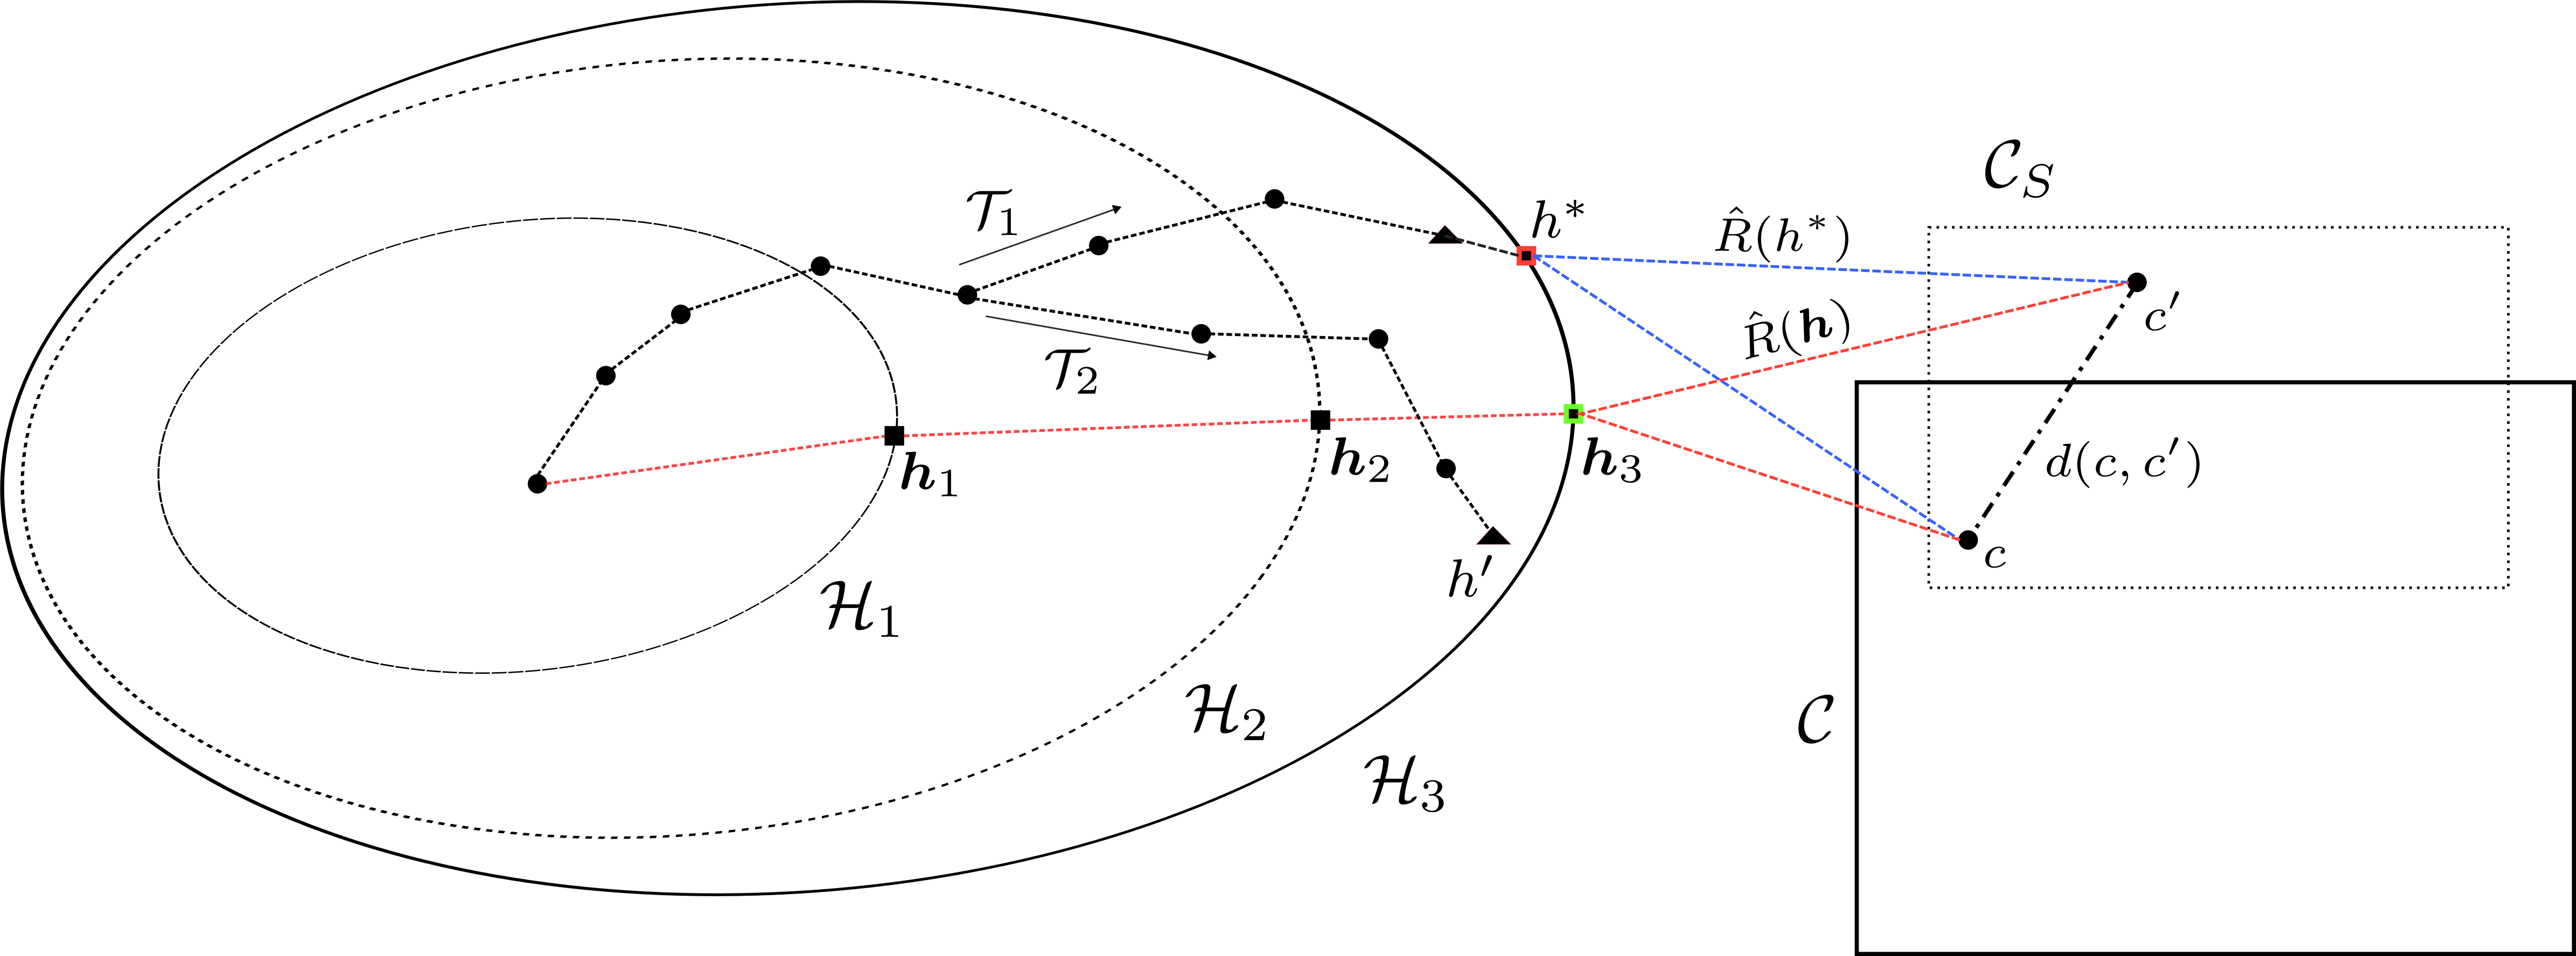
\includegraphics[width=0.9\textwidth]{g10.png}
  \caption{\textbf{Illustrative dynamic of the learning problem.} For an incremental hypothesis space sequence $\mathcal{H}_{1},\mathcal{H}_{2},\mathcal{H}_{3}$, we aim to obtain the procedure $\mathcal{T}$ that would either reach the \textit{generalization solution} $\bm{h}$, or the \textit{empirical solution} $h^{*}$ for a particular hypothesis class, with respect to the concept $c$ and its observed concept $c'$. Model selection hence dictates how an algorithm or procedure than choose the best possible hypothesis to approximate the generalization solution from the empirical solution set. Do notice that here we explicitly state that the data would create a \textbf{proxy concept} that overlaps with the concept class and of some arbitrary `distance' from the true concept by $d(c,c')$. In case the two classes overlap, there still exists the arbitrary distance. Also, we can also observe the intuitive notion of increasing hypothesis class - while it indeed can help in getting closer to the concept class, the somewhat intrinsic property of current learning theory being the relative random procedure class make it probabilistically unstable.}
  \label{fig:statlearnclassical}
\end{figure}

For fixed $\mathcal{H}$, for fixed and sufficiently large $\mathcal{S}$, and no observation (data) errors, the empirical risk is the generalization risk. These two measures between $h$ and $c$ constitute the learning problem, which can also be separated into both cases - either empirical learning or generalization learning, one to minimize $\hat{R}(h)$, and one to minimize $R(h)$. 

\begin{definition}[Empirical learning problem]
    We present the formal form of the empirical learning. Suppose we have a \textbf{target}, $c\in\mathcal{C}$, where $\mathcal{C}$ is an arbitrary concept class that captures targets of the same type. Suppose we are provided a set of observations $\mathcal{S}$. The problem is to use certain algorithm $\mathcal{A}$ using $\mathcal{S}$, to obtain a hypothesis $h^{*}$ for a fixed $\mathcal{H}$ such that: 
    \begin{equation}\label{eq:lp1}
        R(h^{*}) = \min_{h\in\mathcal{H}} \hat{R}(h) = \min_{h\in\mathcal{H}} \underset{x\sim\mathcal{D}, x\in \mathcal{S}}{\mathbb{E}}\:\ell\{h(x),c(x)\}
    \end{equation} 
\end{definition}

The generalization best $\bm{h}$ is also called in literature as the \textit{Bayes model}, such that it reduces the Bayes risk that is the infimum of the generalization risk, $R^{*}=\inf_{h\in \mathcal{H}}R(h)$. The hypothesis $h^{*}$ is often called the \textit{empirical best}, for it being the minimal, finite hypothesis of the lowest loss evaluation on the entire observation space $\mathcal{S}$. There exists no certified assumption regarding whether $h^{*}$ aligns with the minimal generalization error.

\begin{definition}[Generalization learning problem]
    We present the formal form of the generalization learning problem. Suppose we have a \textbf{target}, $c\in\mathcal{C}$, where $\mathcal{C}$ is an arbitrary concept class that captures targets of the same type. Suppose we are provided a set of observations $\mathcal{S}$. Supposed we have an algorithm $\mathcal{A}$ that for fixed hypothesis space $\mathcal{H}$, \eqref{eq:lp1} holds true. The problem is to use certain algorithm $\mathcal{A}'$ such that, under limited availability, to obtain $\bm{h}$, satisfies: \begin{equation}
        R(\bm{h}) = \min_{h\in \mathcal{H}} R(\bm{h}) \leq \{\epsilon\}, \quad \epsilon > 0 
    \end{equation}
    For a set of risk bounds $\epsilon$. If the setting is deterministic, then there exists $\epsilon=0$. 
\end{definition}

Then, we can partially say that generalization problem is an advancement from empirical solution. As such, empirical solution imposes the observed concept, and not the concept itself. This is reflected in modern machine learning landscape, by modelling the concept as distributions, and then using notions such as KL-divergence to measure such relative disparity. 

These two stages of learning procedure comes of as the intrinsic design of machine learning setting. As opposed to interpolation, where empirical learning problem would have to be put into first priority to achieve the best possible point-through model, machine learning leans on approximation more and a separated criterion that is only visible in the learning setting - the fact that we are using $c'$ to extract $c$. This disparity is exactly the \textbf{generalization problem}, of which is then also the goal of machine learning, to approximate the general solution using the observed solution. One then can ask what is the difference between the two notions, and when we can guarantee that both will `converge' to the same point. The process of \textbf{model selection} is then the procedure that will optimize $h\in \mathcal{H}$ to a given target fixture, such as the empirical best. 

One of the major assumption or observation from the point of the hypothesis class, is that the hypothesis cannot know the generalization error. Thereby, the more efficient and often used procedure/algorithm in training, is then the \textit{empirical risk minimization} (ERM) method, minimizing only the empirical risk to the empirical best; then, certain measures to `generalize' this heuristically is apprehended on the hypothesis. The process of model selection is also the place that we get the concept of \textbf{bias-variance tradeoff}. 

Suppose that for a concept class $\mathcal{H}$, we can then partition it to $\mathcal{H}=\bigcup_{k\in \mathbb{N}} \mathcal{H}_{k}$ for finite $k$ hypotheses. Assume that they satisfy the uniform convergence (a very big assumption): 
\begin{equation}
    \forall k \in \mathbb{N}, \quad \underset{S\sim \mathcal{D}^{m}}{\mathbb{P}} \left(\sup_{h\in \mathcal{H}_{k}} R(h) - \hat{R}_{S}(h)\leq \epsilon_{k}(m,\delta)\right) \geq 1- \delta
\end{equation}
for functions $\epsilon_{k}$ satisfies that for all $k$ and $\delta\in (0,1)$, $\lim_{m\to\infty}\epsilon_{k}=0$. One of the major assumption or observation from the point of the hypothesis class, is that the hypothesis cannot know the generalization error. Thereby, the more efficient and often used procedure/algorithm in training, is then the \textit{empirical risk minimization} (ERM) method, minimizing only the empirical risk to the empirical best; then, certain measures to `generalize' this heuristically is apprehended on the hypothesis:
\begin{equation}
        \mathsf{ERM}(h') = \argmin_{h\in \mathcal{H}} \hat{R}(h)
    \end{equation}
Another way is to use the \textit{structural risk minimization} (SRM) method, which add a regularizer $r(\cdot)$ after the empirical error,
\begin{equation}
        \mathsf{SRM}(h') = \argmin_{h\in \mathcal{H}} \hat{R}(h) + \lambda r(h)
    \end{equation}
The regularizer term $r(\cdot)$ takes of its argument the model, and calculate based of certain measure of its complexity. Thereby, the goal is to penalize structures with high complexity and favour simpler designs, in principle.

In this research, we would like to presume the ERM method in question as the famous \textit{gradient descent}. We refer to \cite{achlioptas_stochastic_nodate,ruder_overview_2017} for general view of the algorithm, and \cite{zhang_gradient_2019} for a source on particularly gradient descent algorithm on deep learning models. Nominally, for the $n$th output sequence $w_{n}$, it updates the model to a given path of optimization for $w_{n+1}$ such that 
\begin{equation}
    w_{n+1} = w_{n} - \alpha_{n}\nabla_{w_{n}}(\mathcal{L}(h(x),y))
\end{equation}
for $\alpha_{n}\geq 0$ the step size of the iteration, and with a (potentially) convex function $\mathcal{L}(h(x),y)$ of the hypothesis class $\mathcal{H}$. 

\section{Practical Preliminary}

Previously, we established that at least in said formal setting, generalization errors cannot be known beforehand. Thereby, all of our operations, procedures, processes has to be conducted using the observed data, or the sample space $\mathcal{S}$. A solution to utilize that is to consider the generalization region as the region of \textit{new, unseen observations} that while still is of the same concept $c$, but it is indeed, unseen if the model is never provided of such instances. Hence, it prompts the utilization of limited resources by then to partition the sample space into various subspaces, that would be then fed into the learning process as observational space. This is simply called \textbf{sample set partitioning}. Denoted the number of partition (discrete) as $k$, then for $k=2$, then this is called the \textbf{train-test partition} (or dataset). This contains a dataset $\mathbf{x}_{1}$ and $\mathbf{x}_{2}$ of the same original sample set, such that $\mathbf{x}_{1}/\mathbf{x}_{2}\geq 1$ (one is bigger than another, usually). The ratio does indeed affect the overall running procedure, accordingly.

If $k>3$ and above, we call it the $n$th partitioning. If we further consider the choice of observational spaces being provided, then if $k>3$, and subspaces are chosen randomly, it is called \textbf{cross-validating partition}. The effect of them are fairly well-understood, and we might as well refer to authoritative sources on such issue. 

Based on the above conclusion, the empirical error and generalized error can be re-calculated to fit the general scheme. For $\lvert \mathcal{S}\rvert = m$ and partition $k+p=m$ for train and test partition respectively, 
\begin{equation}
    \hat{R}_{k}(h) = \frac{1}{k} \sum^{k}_{i=1} \ell\{h(x_{i}),c(x_{i})\},\quad \hat{R}_{p}(h_{\mathcal{A}}) = \frac{1}{k} \sum^{p}_{i=1} \ell\{h_{\mathcal{A}}(x_{i}),c(x_{i})\}
\end{equation}
where $h_{\mathcal{A}}$ is the result from the learning algorithm (procedure), for $h^{*}\neq h_{\mathcal{A}}$. Then, the empirical learning seeks to optimize the first term, that is, for the objective 
\begin{equation}
    \underset{h\in \mathcal{H}}{\argmin}\: \hat{R}_{k}(h) = \underset{h\in \mathcal{H}}{\argmin}\:\frac{1}{k} \sum^{k}_{i=1} \ell\{h(x_{i}),c(x_{i})\}
\end{equation}
and the generalization learning as: 
\begin{equation}
    \begin{split}
        \underset{h\in \mathcal{H}}{\argmin}\: \hat{R}_{p}(h_{\mathcal{A}}) 
        & = \hat{R}_{k}(h_{\mathcal{A}}) + \underset{h\in \mathcal{H}}{\argmin}\:\hat{R}_{p}(h_{\mathcal{A}})\\
        & =  \underset{h\in \mathcal{H}}{\argmin}\: \left[\frac{1}{k} \sum^{k}_{i=1} \ell\{h_{\mathcal{A}}(x_{i}),c(x_{i})\} + \frac{1}{k} \sum^{p}_{i=1} \ell\{h_{\mathcal{A}}(x_{i}),c(x_{i})\}\right]\\
        & = \underset{h\in \mathcal{H}}{\argmin}\: \left[\epsilon + \frac{1}{k} \sum^{p}_{i=1} \ell\{h_{\mathcal{A}}(x_{i}),c(x_{i})\}\right]
    \end{split}
\end{equation}
By the definition order, the generalization error can only be calculated post-$\mathcal{A}$. Hence, we often called the empirical, or $\mathsf{ERM}$-generalizer case to be dynamic, and the solution for $\mathsf{ERM}$ is tested statically on generalization set. This partition of order of computation though, brings up the problem of updating factors and others contributing potential that will damage or diffuse the measure. 

For cross-validation and other randomize partition, the formulation requires more care in the notion by itself. The structural risk minimization scheme dilemma can be understood from the above consideration naturally. We have effectively defined the two proxies, \textbf{heuristic empirical risk} and \textbf{heuristic generalization risk}. 

%\begin{figure}[htb]
%    \centering
%    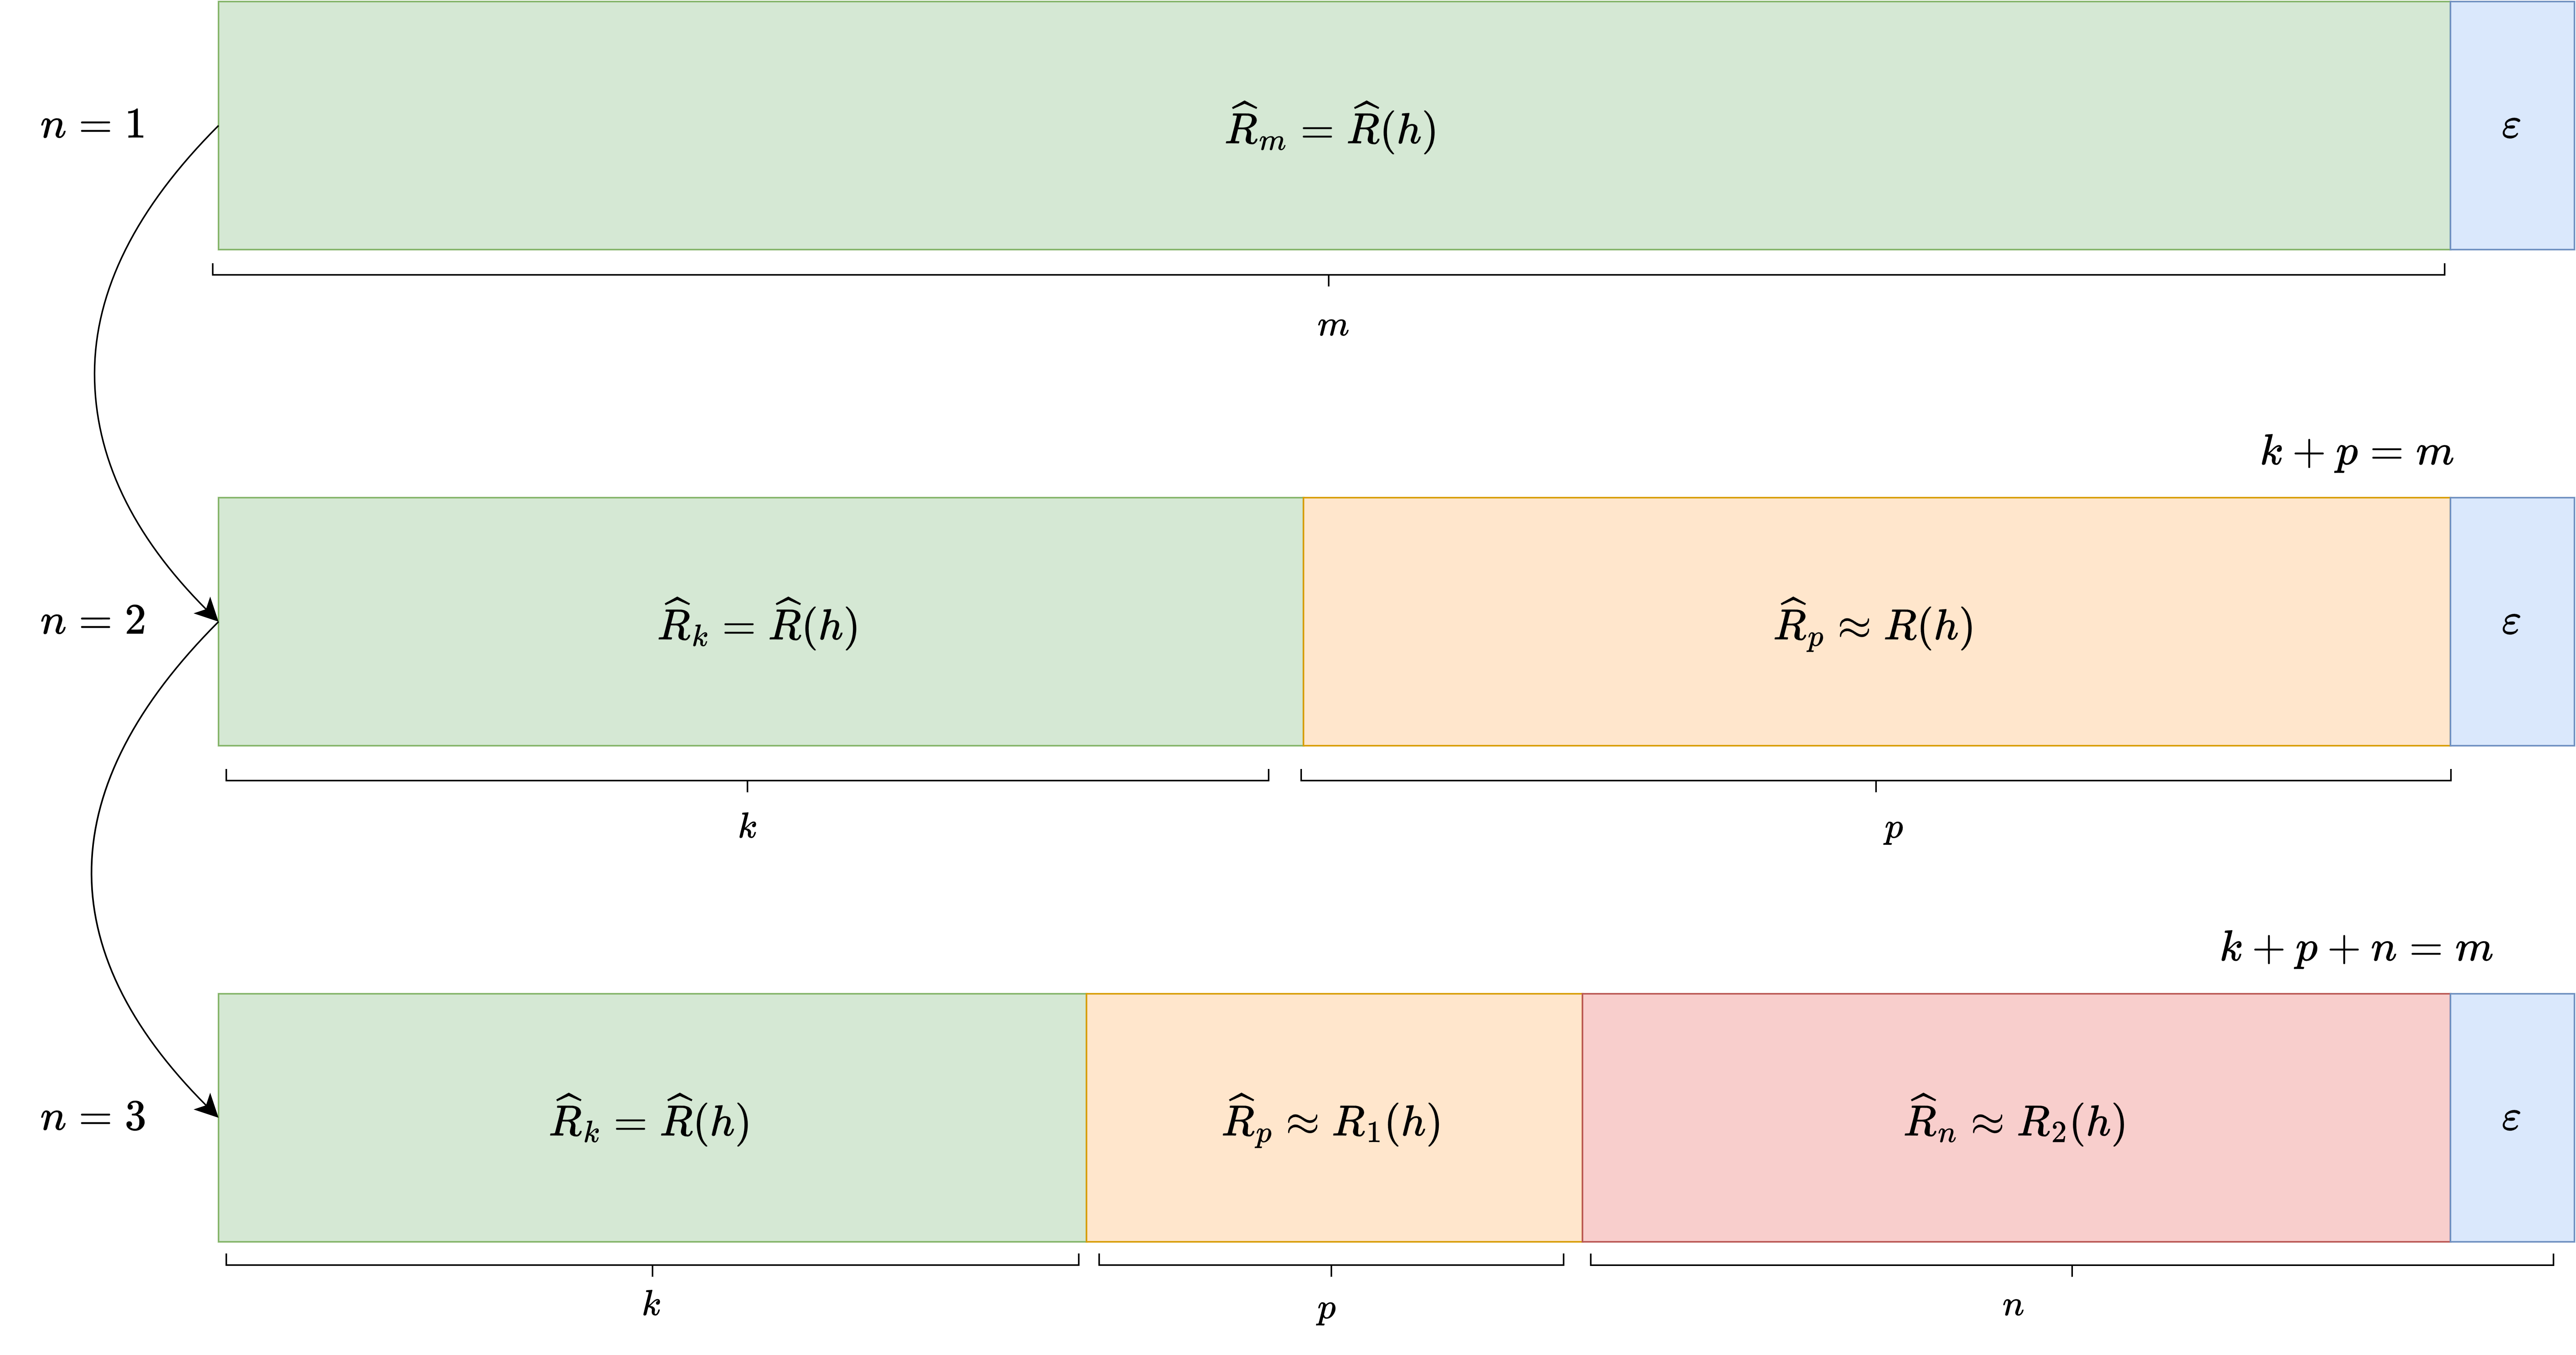
\includegraphics[width=0.7\textwidth]{mamamia.png}
%    \caption{Partitioning process and its error potential consideration. We assume each partition includes the irreducible error $\epsilon$ accompanied by the $n$ %partition, belongs to the furthest partitioning set. Within every increasing partition, for supposed distributed data (unordered data), the generalization %risk is further decomposed.}
%\end{figure}

\begin{SCfigure}[0.4][htb]
  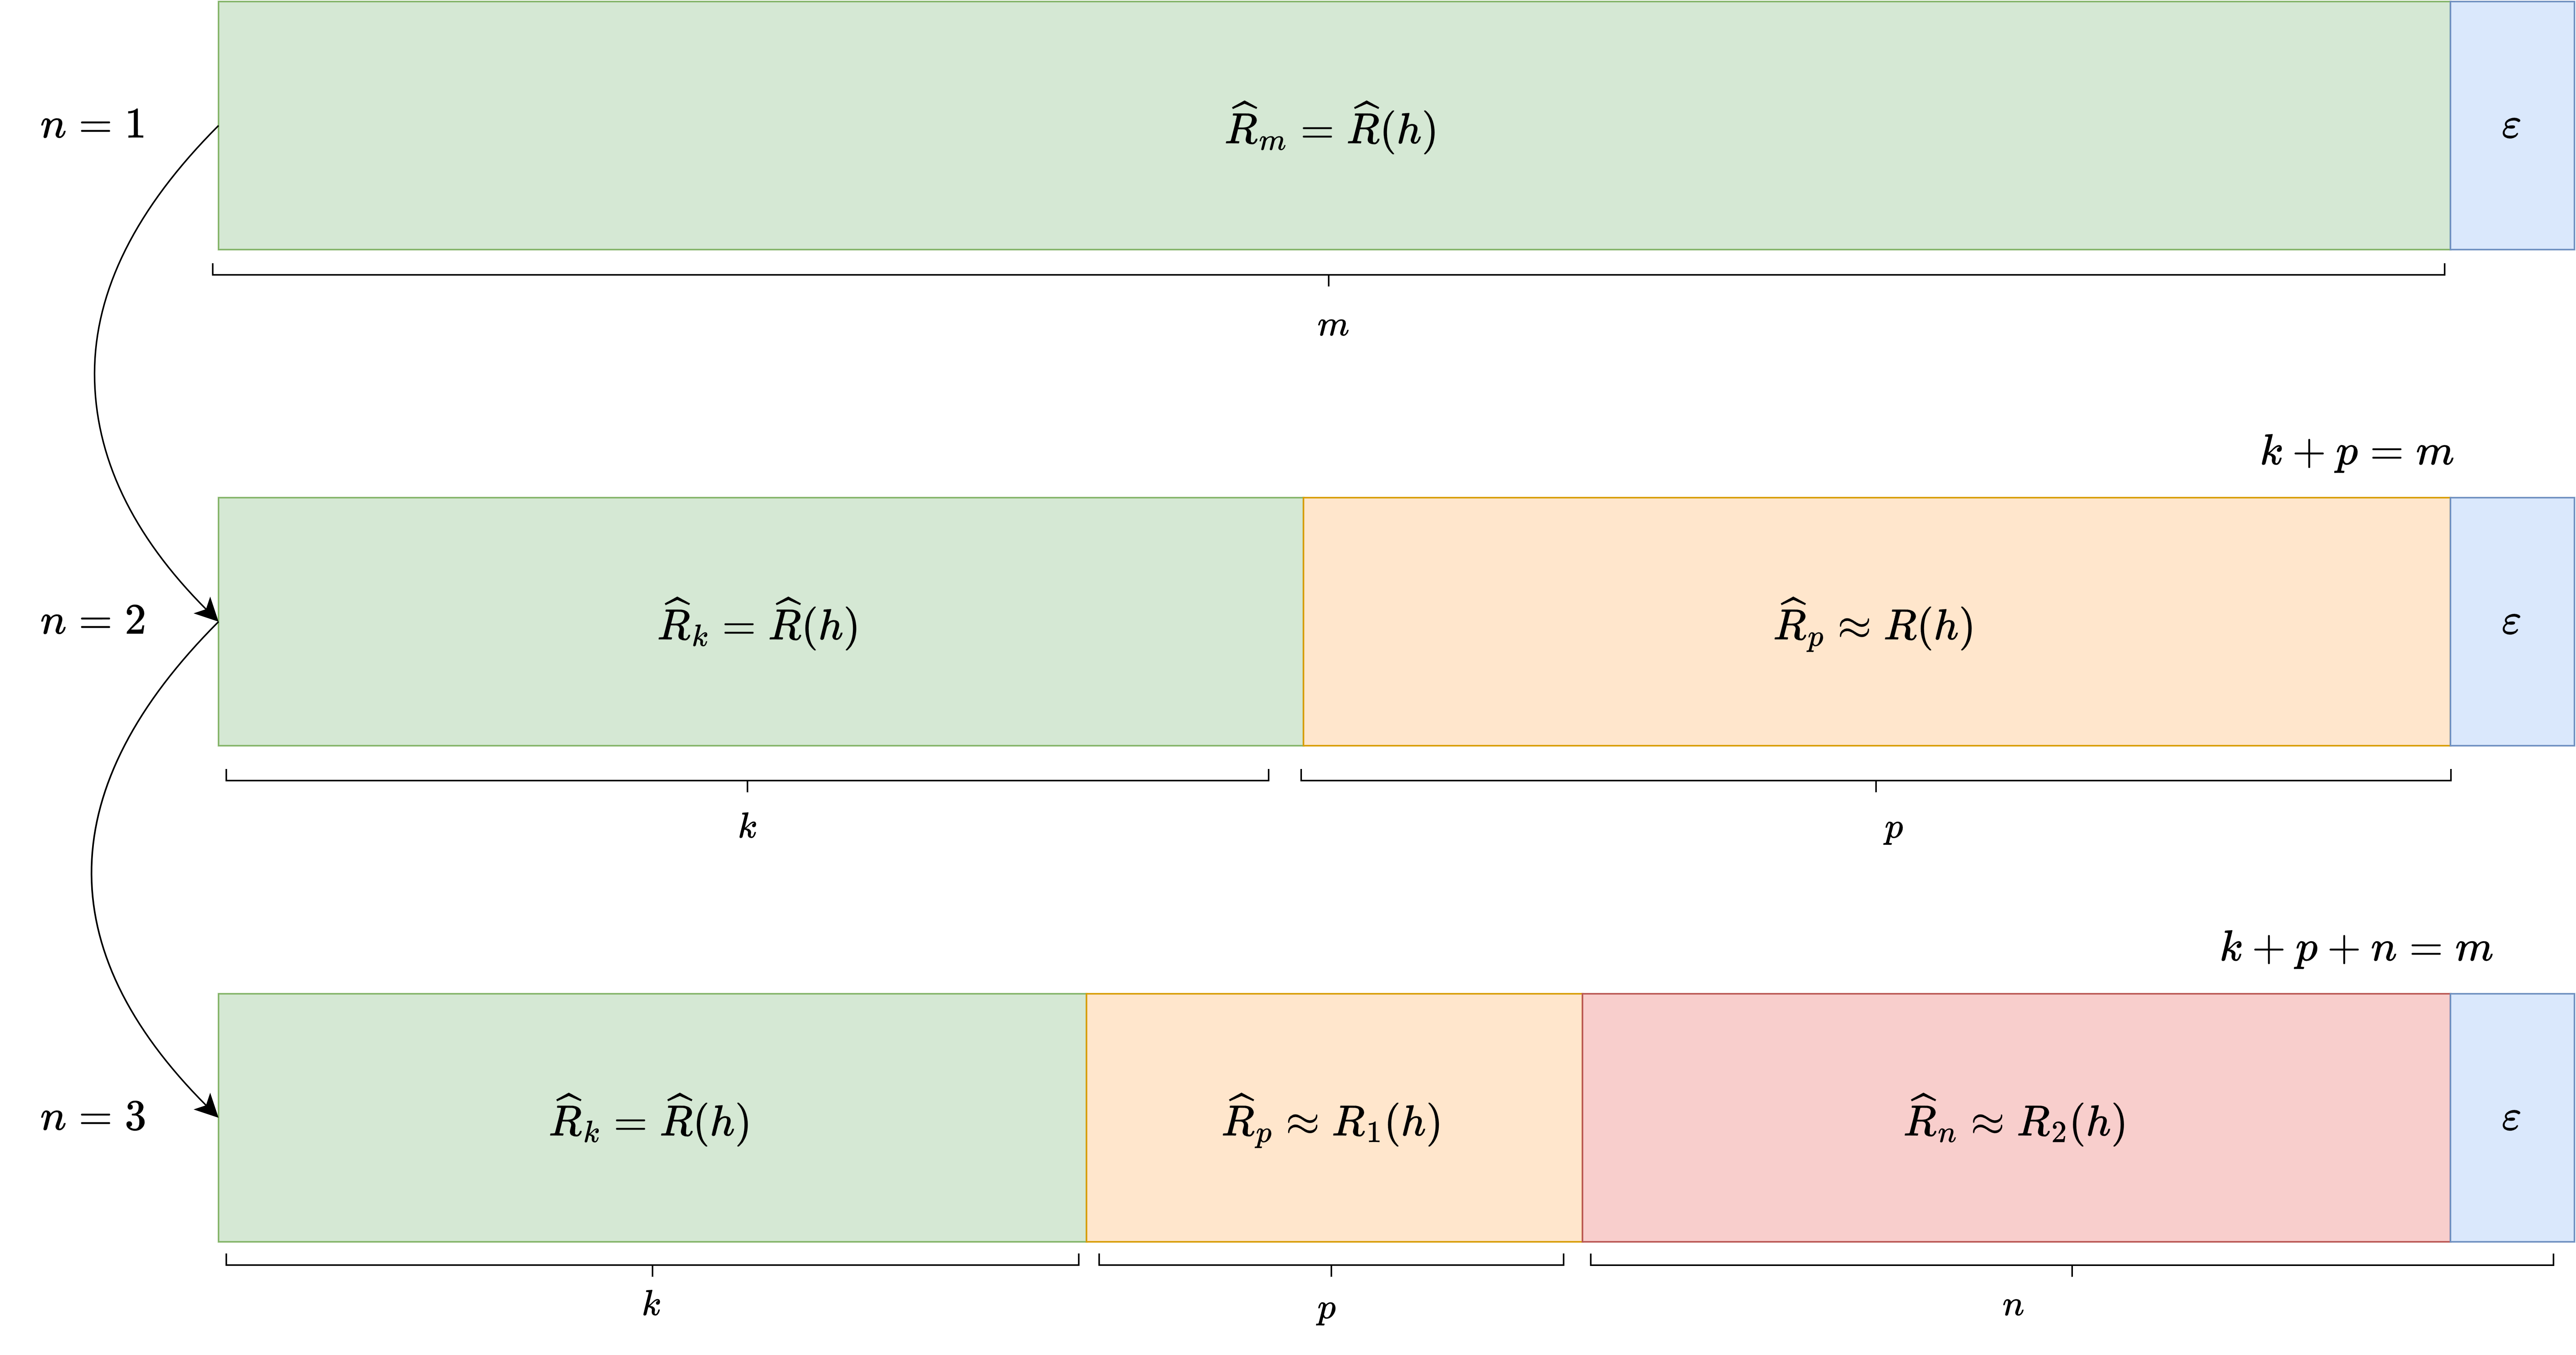
\includegraphics[width=0.6\textwidth]{mamamia.png}
  \caption{\textbf{Partitioning process and its error potential consideration.} We assume each partition includes the irreducible error $\epsilon$ accompanied by the $n$ partition, belongs to the furthest partitioning set. Within every increasing partition, for supposed distributed data (unordered data), the generalization risk is further decomposed.}
\end{SCfigure}

While they are effective as a pair, just as Figure~\ref{fig:randomwalk_descent} illustrated, overly optimizing the path can lead to it in general, be fairly ineffective. On the flip side, not sufficiently optimizing the path will lead to sub-average result, leading to adverse relation. Furthermore, since $\mathcal{S}$ might not, in general, be representative of the population that depicts $c$, the form $c'$ created from observations of $c$-generated space (we call this the \textbf{observed concept} to the true concept) might be skewed, leading to adverse effect. From there, we gain the notion of \textbf{overfitting} and \textbf{underfitting} under the constraints of limited knowledge and reduced concept space to the observation space, relative to the true concept itself. It is also from here that the proxy concepts of \textbf{bias} and \textbf{variance} are introduced to construct the bias-variance tradeoff, and subsequently, the phenomena of double descent. 

Another point to note is also the way of partitioning and location of the data. As we have suggested, data comes in a variety of range, of which we can directly infer from using the supremum set and the infimum element, given particular structure and encoding space. Denoted by $\mathbf{r}_{\mathcal{S}}$, it is responsible for the partitioning strength of the dataset on its own. Then, partitioning must also take the randomization chance, or the distribution and distinctive ordering of the dataset. That is, the metadata related to the dataset must also be configured, as suggestibly, there would be some observable behaviours typically available with, for example in permutation or linear ordering of data by magnitude and expression range. If that is the case, and the data is discretely fragmented, but not diffused in the manner that spread out the missing information all around the dataset, the result would be entirely different, and it would influence the generalization error, heuristically, far more than what is realized. Thereby, there then exists two fundamental polarity: either it is the \textit{totally ordered set}, or it is \textit{randomized uniform aberration}, for any given observation space. 

\subsection{Datasets and its potential effects}

The effect that data has on the model should also be taken into account, as of fact. As far as we are concerned of, the shape, practical system that the dataset gives the setting, the factors running into the dataset, the choice of the dataset being sampled, selected in partitions, and other factors must also be analysed. Without such, we leave `gaps' in which sensitive, potentially chaotic behaviours might occur frequently and would not be identified, or being classified into irreducible errors, static of the learning setting. As such, we might as well list a few potential points of interest. 
\begin{enumerate}[itemsep=1pt,topsep=0.5pt]
  \item \textbf{Data distribution}: the distribution of the dataset itself affects how the concept is represented in the space. If the representation space created by using the data is large, but sparse, then the condition would make for some behaviours to occur more easily. This is one degree of freedom of the system setting. If the dataset spread is low, yet the data is very volatile, then it will lead to inconclusive picture of the actual concept, hence introducing new behaviours on the now unknown region of the distribution. As such, the majority of those unknown spaces will treat every point there as a potential outlier instead. 
  \item \textbf{Data complexity}: The complexity of the data itself is of interest. In a controlled setting of response-inducing evaluation, identifying behaviours of the model with a glimpse on the data complexity - how the actual data works with the internal mechanics accompanied - is of specific interest, as it can affect some of the majorative effects and chaotic behaviours that occur in the learning process, especially stochastic process and probabilistic optimization patterns. 
  \item \textbf{Data partitions}: The partitioning of data in the previously mentioned sample partitioning section might give rise to previously observed behaviours, as well as explaining particular volatility when changing the test partitioning set. The ordering of the dataset also helps in such regard. 
\end{enumerate}
It is also worth to note that since we emphasize the use of dataset partitioning to replicate the empirical-generalization guarantee, it is also then indicative that such partitioning would have its separate way of calculating test error on itself. 

Intuitively, it can be illustrated as followed. Suppose of given two datasets $\mathcal{S}_{1},\mathcal{S}_{2}$, we can trace a pattern, if, for assumption, the partition is $k=10$. If the algorithm $\mathcal{A}$ attempt empirical learning optimization specifically, and best optimize on individual partition $\mathcal{S}_{1}^{(i)}$, then the path toward each and individual partition would potentially be very volatile, depends heavily on the partition randomization, and others factor leading to such. If the algorithm is justified in that sense, to `decelerate' the optimization to a not so tight fit, the generalization would be much better. This is also the reasoning for the technique of \textbf{regularization}, and generalization task. However, again, such procedure cannot help but having volatile dataset itself as a factor of uncertainty. More specifically, the result might work for $\mathcal{S}_{1}$, but for another dataset $\mathcal{S}_{2}$, assuming no intersection, that is, $\mathcal{S}_{1}\cap \mathcal{S}_{2}=\varnothing$, then optimization based on one dataset would not be optimal in another, more so can be counterproductive. This is also used of the reasoning for \textbf{cross-validation} technique, of which aims to stabilize the partitioning. However, analytical analysis suggests a wider role of such, in the wider setting of learning theory, particularly in double descent later on. 
\begin{figure}[htb]
  \centering
  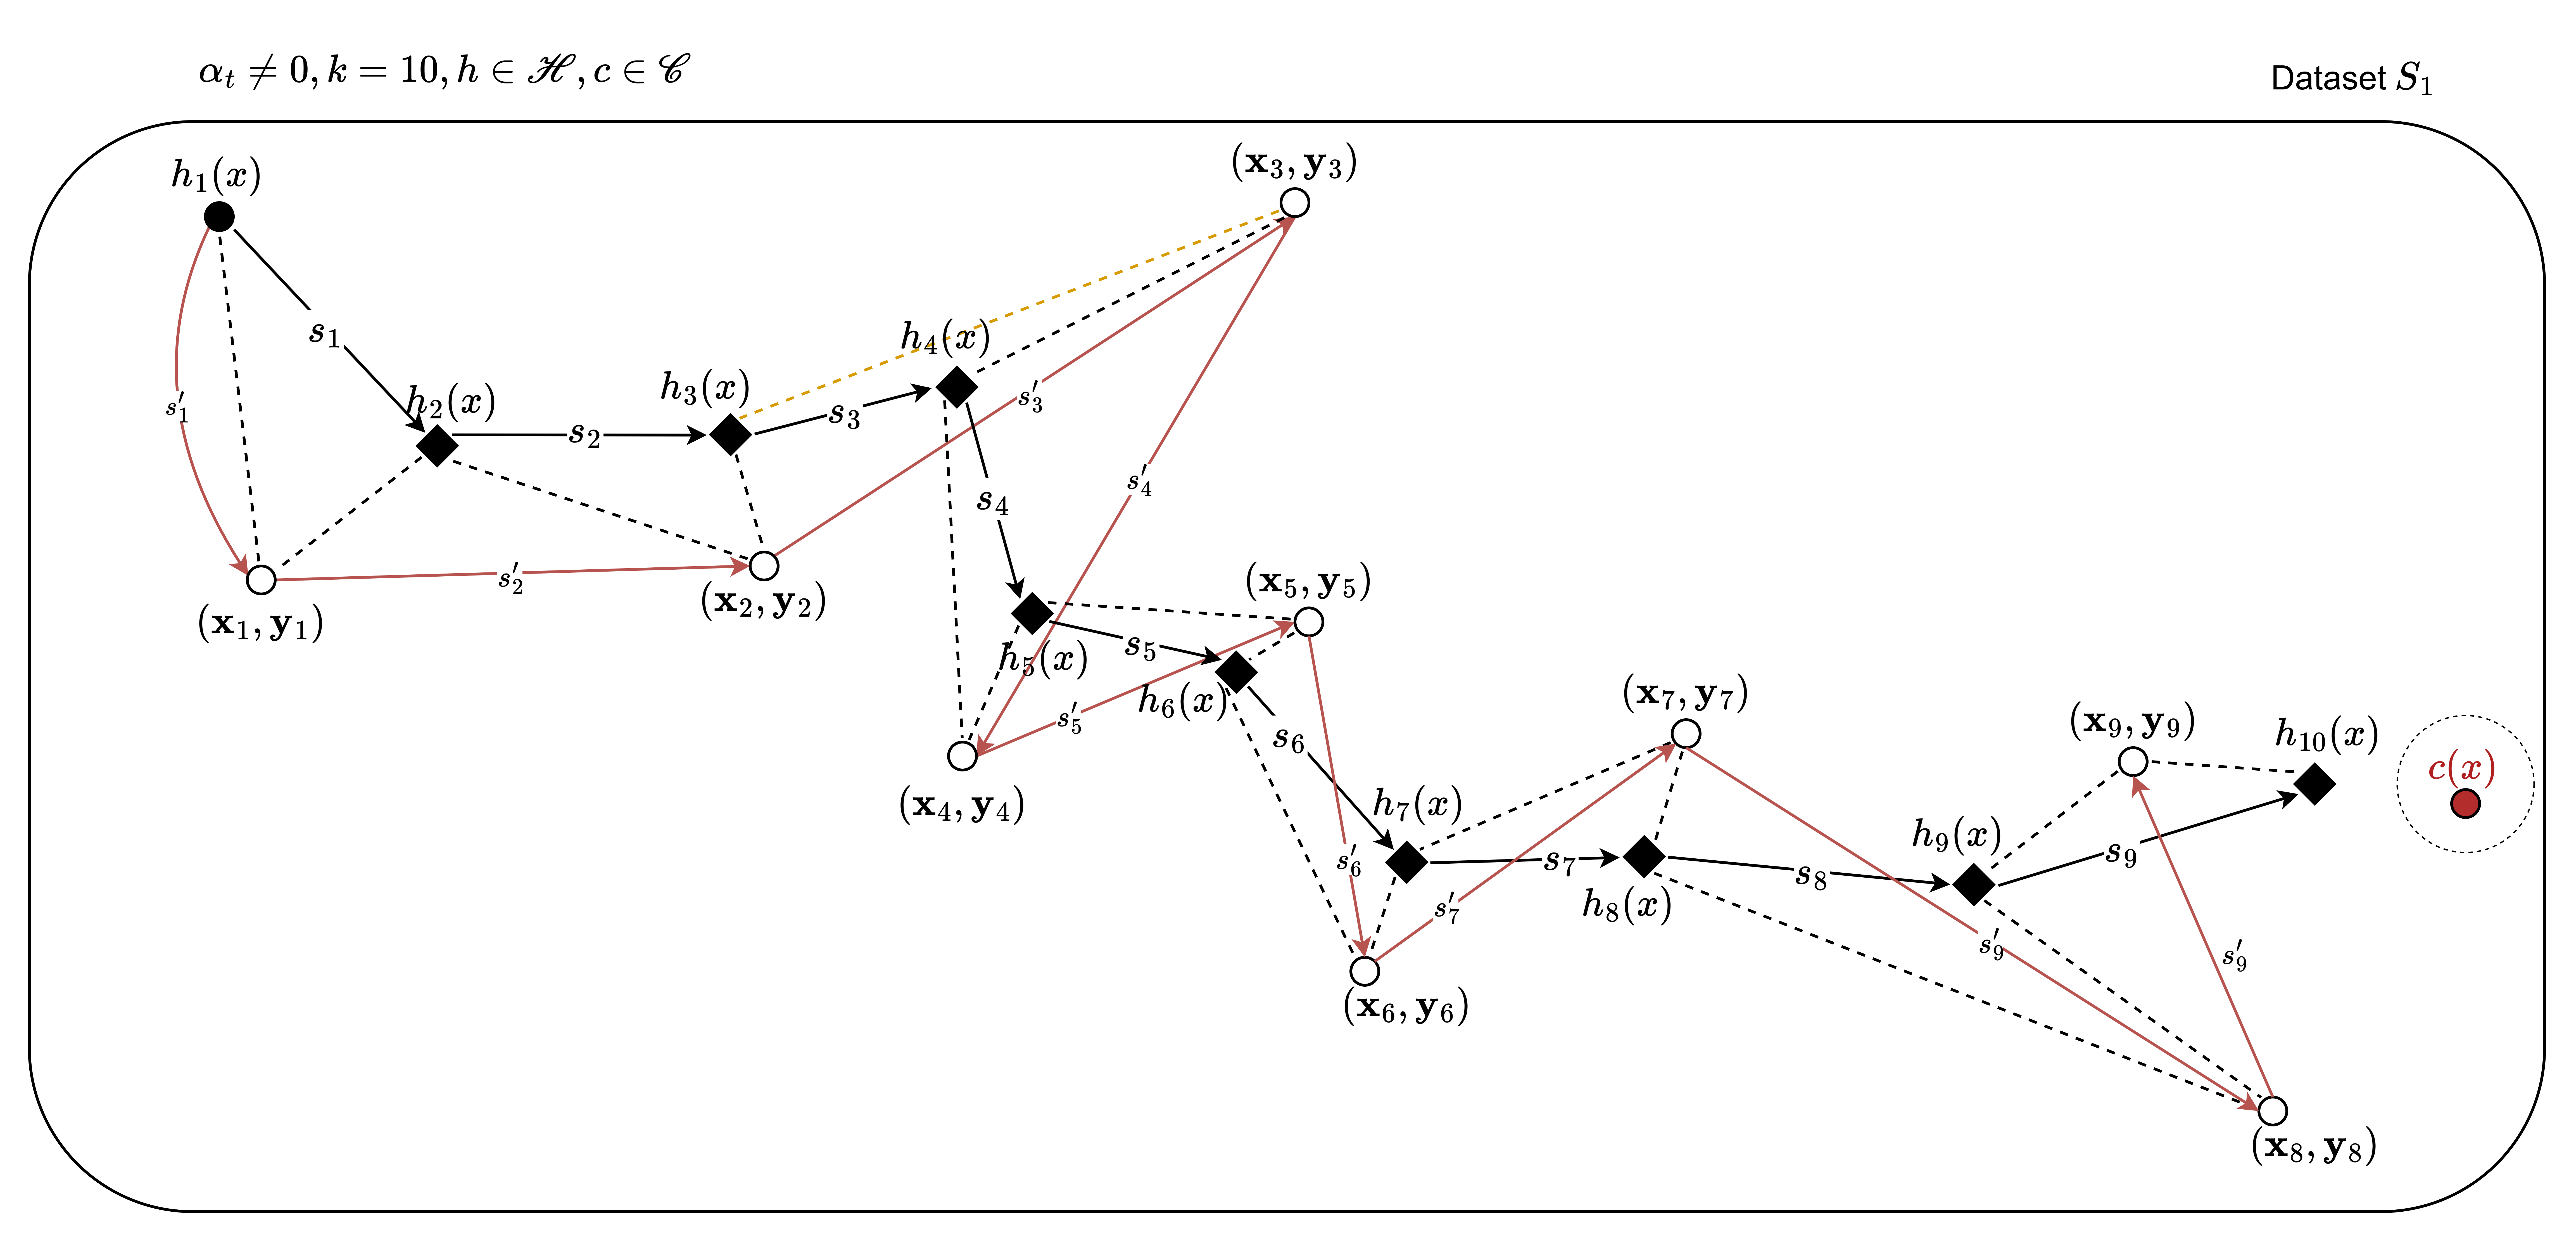
\includegraphics[width=0.7\textwidth]{illustration_descent_algorithm1.png}
  \caption{\textbf{Illustration of dataset optimization path, dataset $\mathcal{S}_{1}$}. From here, we can see the absolute path (in red), the `step-size' path (in black), and the relative step distance between where the model land and the data's supposed suggested shape of $c$. We assume those `snapshot' created by data are within varying noise, however still fall in range of relatively same concept region class. As for the path, we can see that the chosen step size learning is much more stable overall, comparing to the overfitting-like path.}
  \label{fig:randomwalk_descent}
\end{figure}
This behaviour can happen all the same to the dataset's inner partition by itself. Furthermore, different dataset might still have a very bottom-up bound of which it cannot reach certain accuracy metric, intrinsic of the dataset's form. 
\begin{figure}[htb]
  \centering
  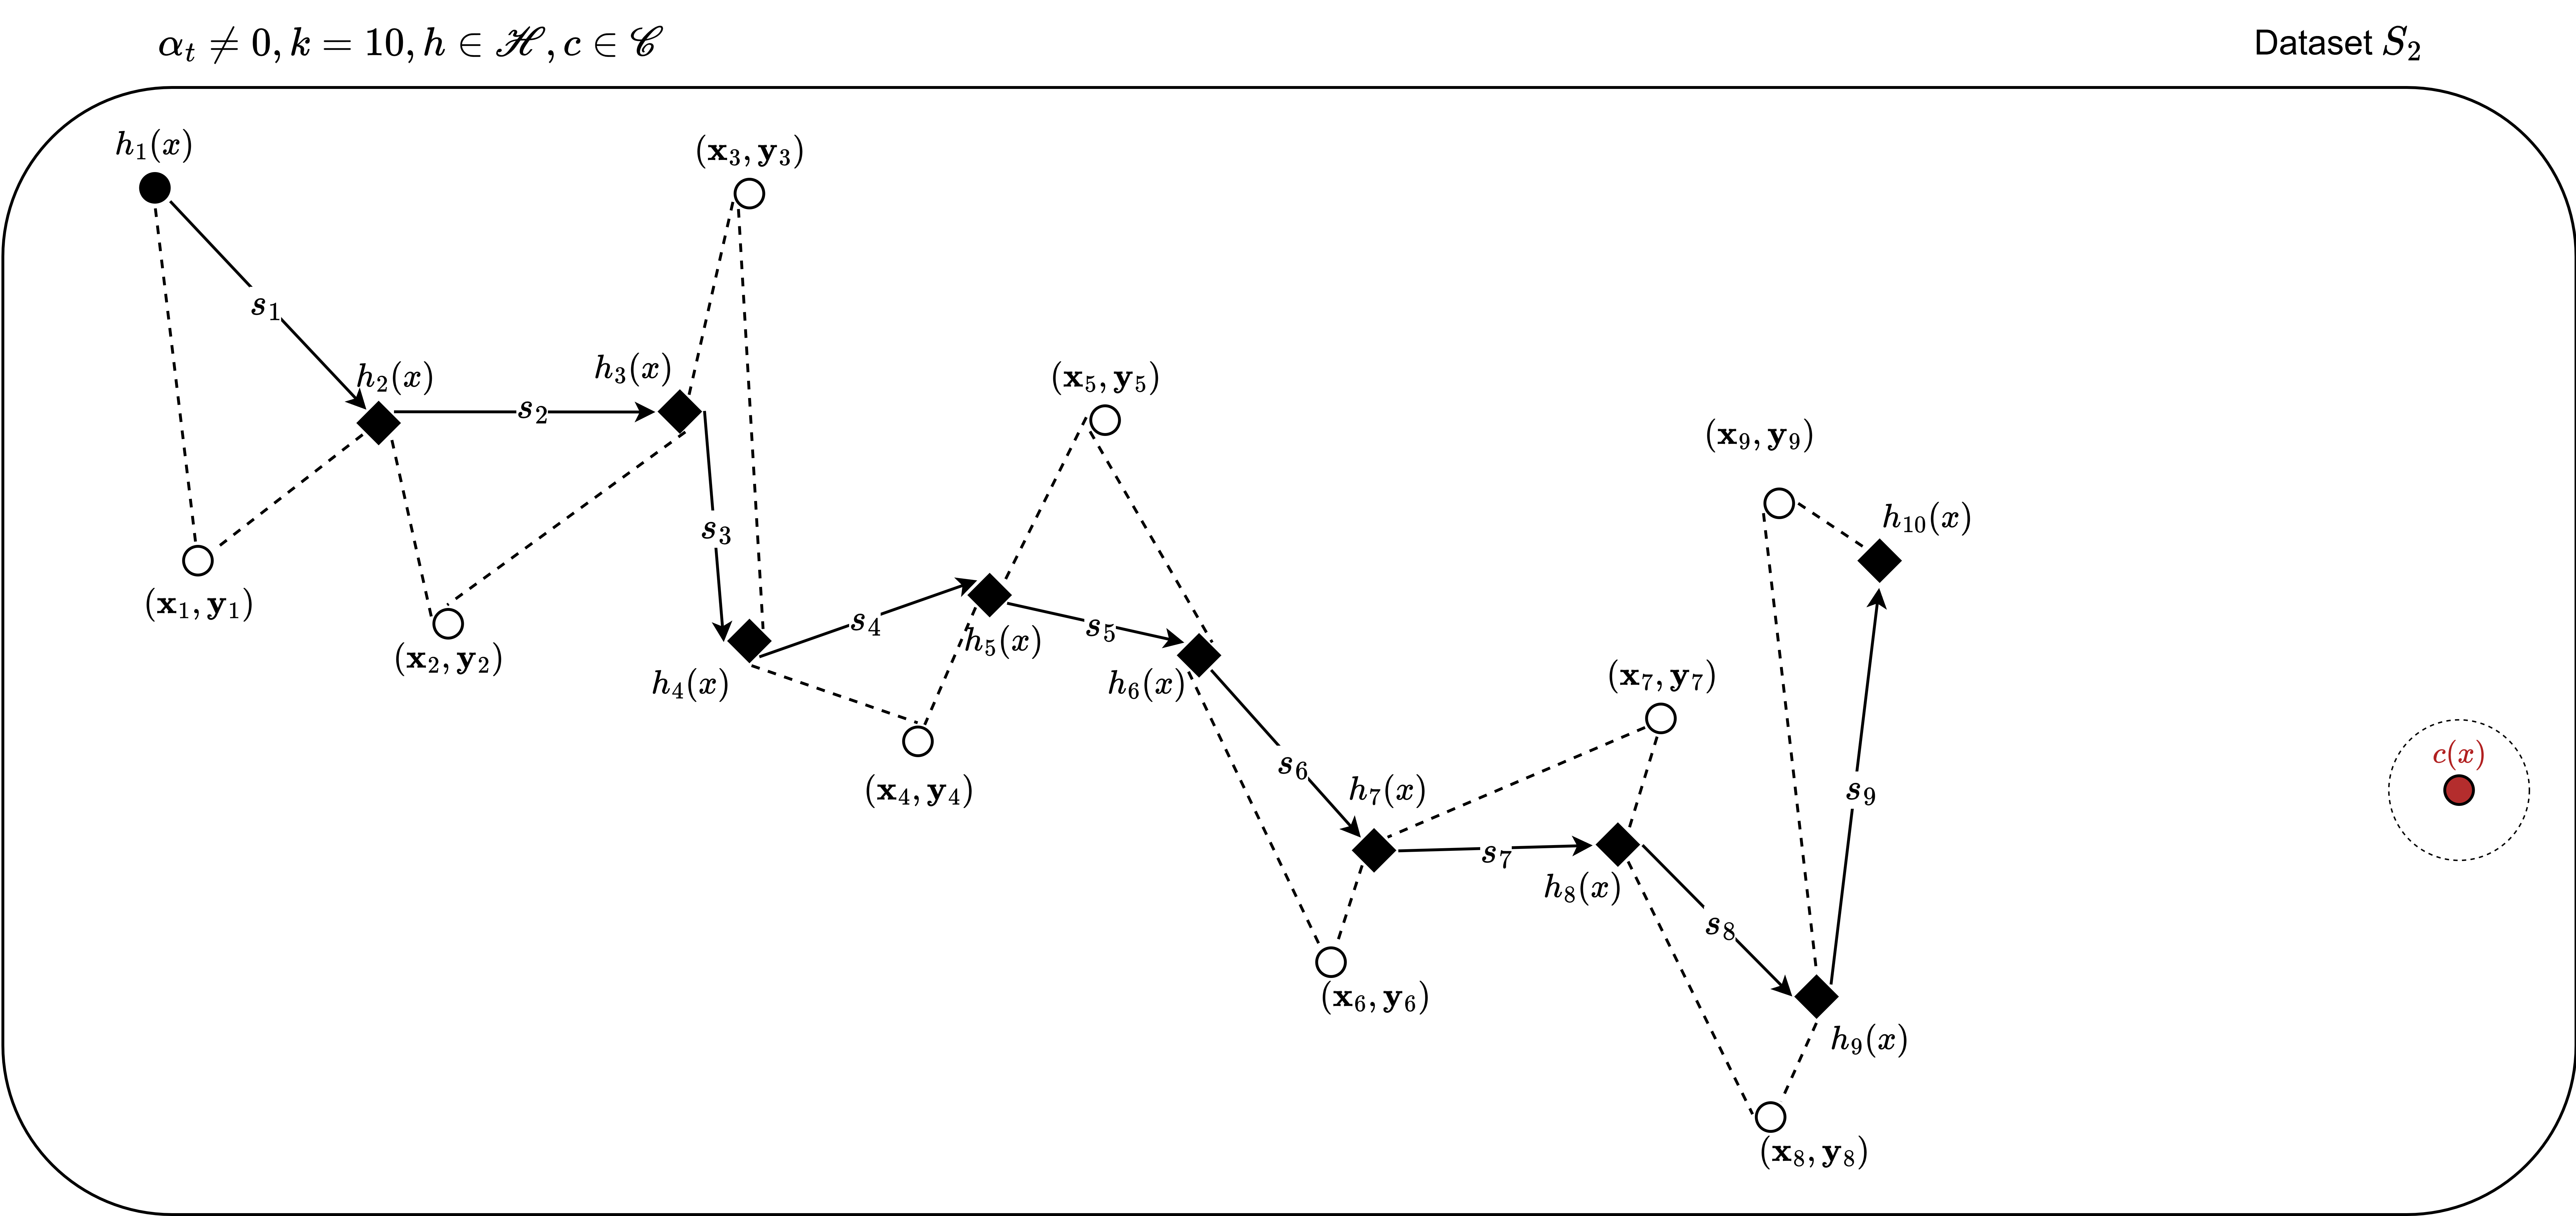
\includegraphics[width=0.7\textwidth]{illustration_descent_algorithm2.png}
  \caption{\textbf{Illustration of dataset optimization path, dataset $\mathcal{S}_{2}$}. Similar to $\mathcal{S}_1$, however, the intrinsic shape and configuration of the dataset makes a further thresholding limit on the approach to $c$, hence specifically under this dataset, we suppose that any sub-partition of $S_{2}$ would not reach certain accuracy measure.}
\end{figure}
\subsection{Overfitting and underfitting}
Under such guise, one understanding about the concept of underfitting and overfitting \cite{gareth_james_introduction_2013} can be reached, using the notion of partitioning. We can define the heuristic for better definition, as followed. 

\begin{definition}[Heuristic empirical risk]
  Given a dataset $\mathcal{S}$ of size $m$, supposedly of the concept $c\in \mathcal{C}$, and the hypothesis $h\in \mathcal{H}$, then the \textbf{heuristic empirical risk} take a partitioning $k<m$ with $k/m\geq 1/2$, hence defining the heuristic empirical loss on $k$, denoted $\hat{R}_{k}(h)$. 
\end{definition}

\begin{definition}[Heuristical generalization risk]
  Given a dataset $\mathcal{S}$ of size $m$, supposedly of the concept $c\in \mathcal{C}$, and the hypothesis $h\in \mathcal{H}$. Fixed $\hat{R}_{k}(h)$, for the final optimization of algorithm $\mathcal{A}$, then the \textbf{heuristic generalization risk} take the remaining 2-partition of portion $p=k-m$, hence defining the heuristic generalization loss on $p$, denoted $\hat{R}_{p}(h_{\mathcal{A}})$. 
\end{definition}
The two heuristic definition however, can be noted to not be equal to the true generalization risk - empirical risk pair in reality. Nevertheless, one can then define overfitting and underfitting in such manner. 
\begin{definition}[Underfitting]
  A model $h$ is called \textbf{underfitting} if for a constant $\epsilon > 0$ chosen for the setting, then $\hat{R}_{k}(h)>\epsilon$, $\hat{R}_{p}(h_{\alpha})> \epsilon$ over the entire observation space. 
\end{definition}
Usually, underfitting is defined to be such that test error is smaller than training error partition, however, we do not think that is a good definition. Especially since, at least in this setting, the empirical error under algorithm $\mathcal{A}$ is reduced to the representative smallest error that $\mathcal{A}$ can achieve on that particular model, within particular setting of $h$, then come the heuristic generalization error. Considering also that $k/m\geq 1/2$, that is, at least the training partition is half of the observation set, then only under very specific case will $\hat{R}_{p}(h_{\alpha})$ be smaller than $\hat{R}_{k}(h)$, statistically speaking. Thence this line of thought also reinforces the idea that both of them will be larger than the threshold $\epsilon$. Usually, heuristically, this threshold of error is $0.3$, normalized. Next, we define the notion of overfitting. 

\begin{definition}[Overfitting]
  A model $h$ is called \textbf{overfitting} if there exists a specific constant $\epsilon>0$ chosen for the setting, such that $\hat{R}_{k}(h)<\epsilon$, $\hat{R}_{p}(h_{\alpha})> \epsilon$ over the entire observation space.
\end{definition}
Namely, this mean that the static learning makes the generalization error worse. This draws the analogy of the student - studying explicitly for the past paper tests, yet unaware of the larger margin of questions in the large set of the test paper pool, leading to subpar performance. Similarly, overfitting is theorized to be fitting too fit to the reduced observation space - hence when it comes to the generalization observation space, it fails within such heuristic. The notion works on the mask of the risks, $\hat{R}_{k}$ and $\hat{R}_{p}(h_{\alpha})$. 

\clearpage
\section{Bias-variance tradeoff}

Bias-variance tradeoff comes off from a statistical approach, predate machine learning by itself. The theory that bias and variance often come in to conjunction is \textbf{Estimation theory}, of which there exists an estimator $\hat{\theta}$ that use a set of observations, to estimate the concept, or the underlying mechanics of certain system that outputted the observation set, by the \textbf{probabilistic perspective} - that is, it is governed by appearance by an independently and identically distributed process of parameterized probability $\theta\in \Theta$. Here, parameterized means being expressed by a set, often finite, of parameters, by \cite{LehmannCasella_theory_1998,liam_statistics_2005}. 
\subsection{Statistical origin}
As we have said, the notion comes from statistical analysis. In such, there are two important functions associated with any estimator $\hat{\theta}$ that are useful as a thumbnail sketch on how well the estimator is doing (\cite{liam_statistics_2005}), the \textit{bias} and the \textit{variance}. Classically, estimation theory is concerned of the problem of data sample estimation on continuous real line $\mathbb{R}$. As such, the ultimate goal of classical estimation theory is the minimization of the estimator mean square error (MSE), that is given as 
\begin{equation}
  \mathsf{MSE}(\hat{\theta}) \triangleq \mathbb{E}_{y} \lvert \lvert \hat{\theta} - \theta \rvert \rvert^{2} = \mathbb{E}_{y} \lvert\lvert z(y) - \theta \rvert \rvert^{2}
\end{equation}
where $y$ is the observation set by notation, and $\hat{\theta}=z(y)$ is the estimator of interest. Then, the bias and variance is defined to be
\begin{equation}
  \mathsf{Bs}(\hat{\theta}) = \lvert\lvert \mathbb{E}_{y} \{\hat{\theta} - \theta\}\rvert\rvert, \quad \mathsf{Var}(\hat{\theta}) = \mathbb{E}_{y} \lvert\lvert \hat{\theta} - \mathbb{E}_{y} \{\hat{\theta}\}\vert\rvert^{2}
\end{equation}
This prompted a tradeoff, in which for the mean squared error the \textbf{minimum mean squared error} (MMSE) estimator would consider the bias and variance for every value of the parameterized descriptor $\theta$. The best strategy potentially can be employed is then to reduce the variance of the model. This is rationalized as because for estimation theory in general, the bias term is unrealizable because it depends on the measure of the true concept. Based on the probabilistic interpretation, the true concept, or its true parameters governing the probabilistic sampling process cannot be learned, and hence the term bias can be at best approximated, with varied degree of accuracy. The limitation (\cite{piera_sample_2005,MkayPretenceSignalStatistics1993}) suggests to focus uniquely on unbiased estimators holding that $\mathsf{Bs}(\hat{\theta})=0$. Thus, the estimator mean square measure is equal to its variance, and the resulting estimator is then referred to as the minimum variance unbiased (MVU) estimator by \cite{MkayPretenceSignalStatistics1993}. 

In modern literature, the analysis of machine learning model and the introduction of such bias-variance concept for model selection criterion first came from \cite{6797087}. Of a later date, there are many interpretations, and similar notions of such tradeoff comes from both statistical learning theory and his original paper, which is used extensively among modern machine learning practicians. 
\subsection{Precursor (Geman et al., 1992)}

The original definition of bias-variance tradeoff by \cite{6797087} is first constructed using the means-square error, which is regarded as a normal measure in the real encoding space. Their approach is to justify bias-variance via decomposition of the loss function $\ell$, for such to find an alternative reasonable form of such loss landscape. Suppose of a regression problem to construct a hypothesis function $f(x)$ from $(x_{1},y_{1},\dots,x_{N},y_{N})$ for the purpose of generalization - that is, predicting unseen variational values for different pair $(x_{j}, \mathord{?})$ such that $\mathord{?}=y_{j}+\epsilon$ for a conceivable implicit error. To be explicit about the relation of this problem, or $f$ on the given data $\mathcal{D}=\{(x_i, y_i)\mid i \leq N\}$, denote $f(x;\mathcal{D})$ instead of $f$, the natural mean-square measure as a predictor is: 
\begin{equation}
    \mathcal{M}(f,y) = \mathbb{E} \left[((y-f(x;\mathcal{D})))^{2}\mid x, \mathcal{D}\right] 
\end{equation} for $\mathbb{E}[\cdot]$ the expectation wrt to a distribution $P$. Decomposing the right-hand side, we have: 
\begin{equation}
    \mathcal{M}(f,y) = \mathbb{E} \left[((y-f(x;\mathcal{D})))^{2}\mid x, \mathcal{D}\right] = \mathbb{E}\left[(y-\mathbb{E}[y\mid x])^{2}\mid x,\mathcal{D}\right] + (f(x;\mathcal{D})-\mathbb{E}[y\mid x])^{2}
\end{equation}
Here, $\mathbb{E}\left[(y-\mathbb{E}[y\mid x])^{2}\mid x,\mathcal{D}\right]$ does not depend on $\mathcal{D}$, but simply the statistical variance of $y$ given $x$. The term $(f(x;\mathcal{D})-\mathbb{E}[y\mid x])^{2}$ is considered a natural measure of effectiveness on $\mathbb{R}^{n}$ as a singular predictor of $y$. Now, for $\mathbb{E}_{\mathcal{D}}\left[(f(x;\mathcal{D})-\mathbb{E}[y\mid x])^{2}\right]$ which depends on the training set $\mathcal{D}$ in its computation, is decomposed into the form of \textit{bias-variance decomposition} terms, by derivation: 
\begin{equation}
    \begin{split}
        \mathbb{E}_{\mathcal{D}} \left[(f(x;\mathcal{D})-\mathbb{E}[y\mid x])^{2}\right] & = \underbrace{\left\{ \mathbb{E}_{\mathcal{D}}[f(x;\mathcal{D})] - \mathbb{E}[y\mid x] \right\}^{2}}_{\text{bias term}} + \underbrace{\mathbb{E}_{\mathcal{D}} \left\{(f(x;\mathcal{D})- \mathbb{E}_{\mathcal{D}}[f(x;\mathcal{D})])^{2}\right\}}_{\text{variance term}}
    \end{split}
\end{equation}

We summarize this in the following statement. 

\begin{theorem}[Bias-variance decomposition]
    Suppose the model $f(x;\mathcal{D})$ for the data $\mathcal{D}=(x_i, y_i)$ and its parameter $x$ is defined. For $y_{i}$ of the target concept's responses $y$, and consider a regression problem with the loss measure $\mathcal{M}(f,y)$ of mean squared risk, the following statement is true: \begin{equation}
        \mathbb{E}\big[\mathcal{M}(f,y)\big] = \mathcal{B}(f,y) + \mathcal{V}(f,y) + \mathbb{E}\Big[\mathbb{E} \left[((y-f(x;\mathcal{D})))^{2}\mid x, \mathcal{D}\right]\Big]
    \end{equation}
    for $\mathbb{E}[\:\cdot\mid x, \mathcal{D}]$ any expression with dependencies on $x$ and $\mathcal{D}$. The bias and variance term is subsequently expressed by 
    \begin{align}
        \mathcal{B}(f,y) = \underbrace{\left\{ \mathbb{E}_{\mathcal{D}}[f(x;\mathcal{D})] - \mathbb{E}[y\mid x] \right\}^{2}}_{\text{bias }}, \quad \mathcal{V}(f,y) =\underbrace{\mathbb{E}_{\mathcal{D}} \left\{(f(x;\mathcal{D})- \mathbb{E}_{\mathcal{D}}[f(x;\mathcal{D})])^{2}\right\}}_{\text{variance}}
    \end{align}
\end{theorem}

\begin{SCfigure}[0.5][htb]
  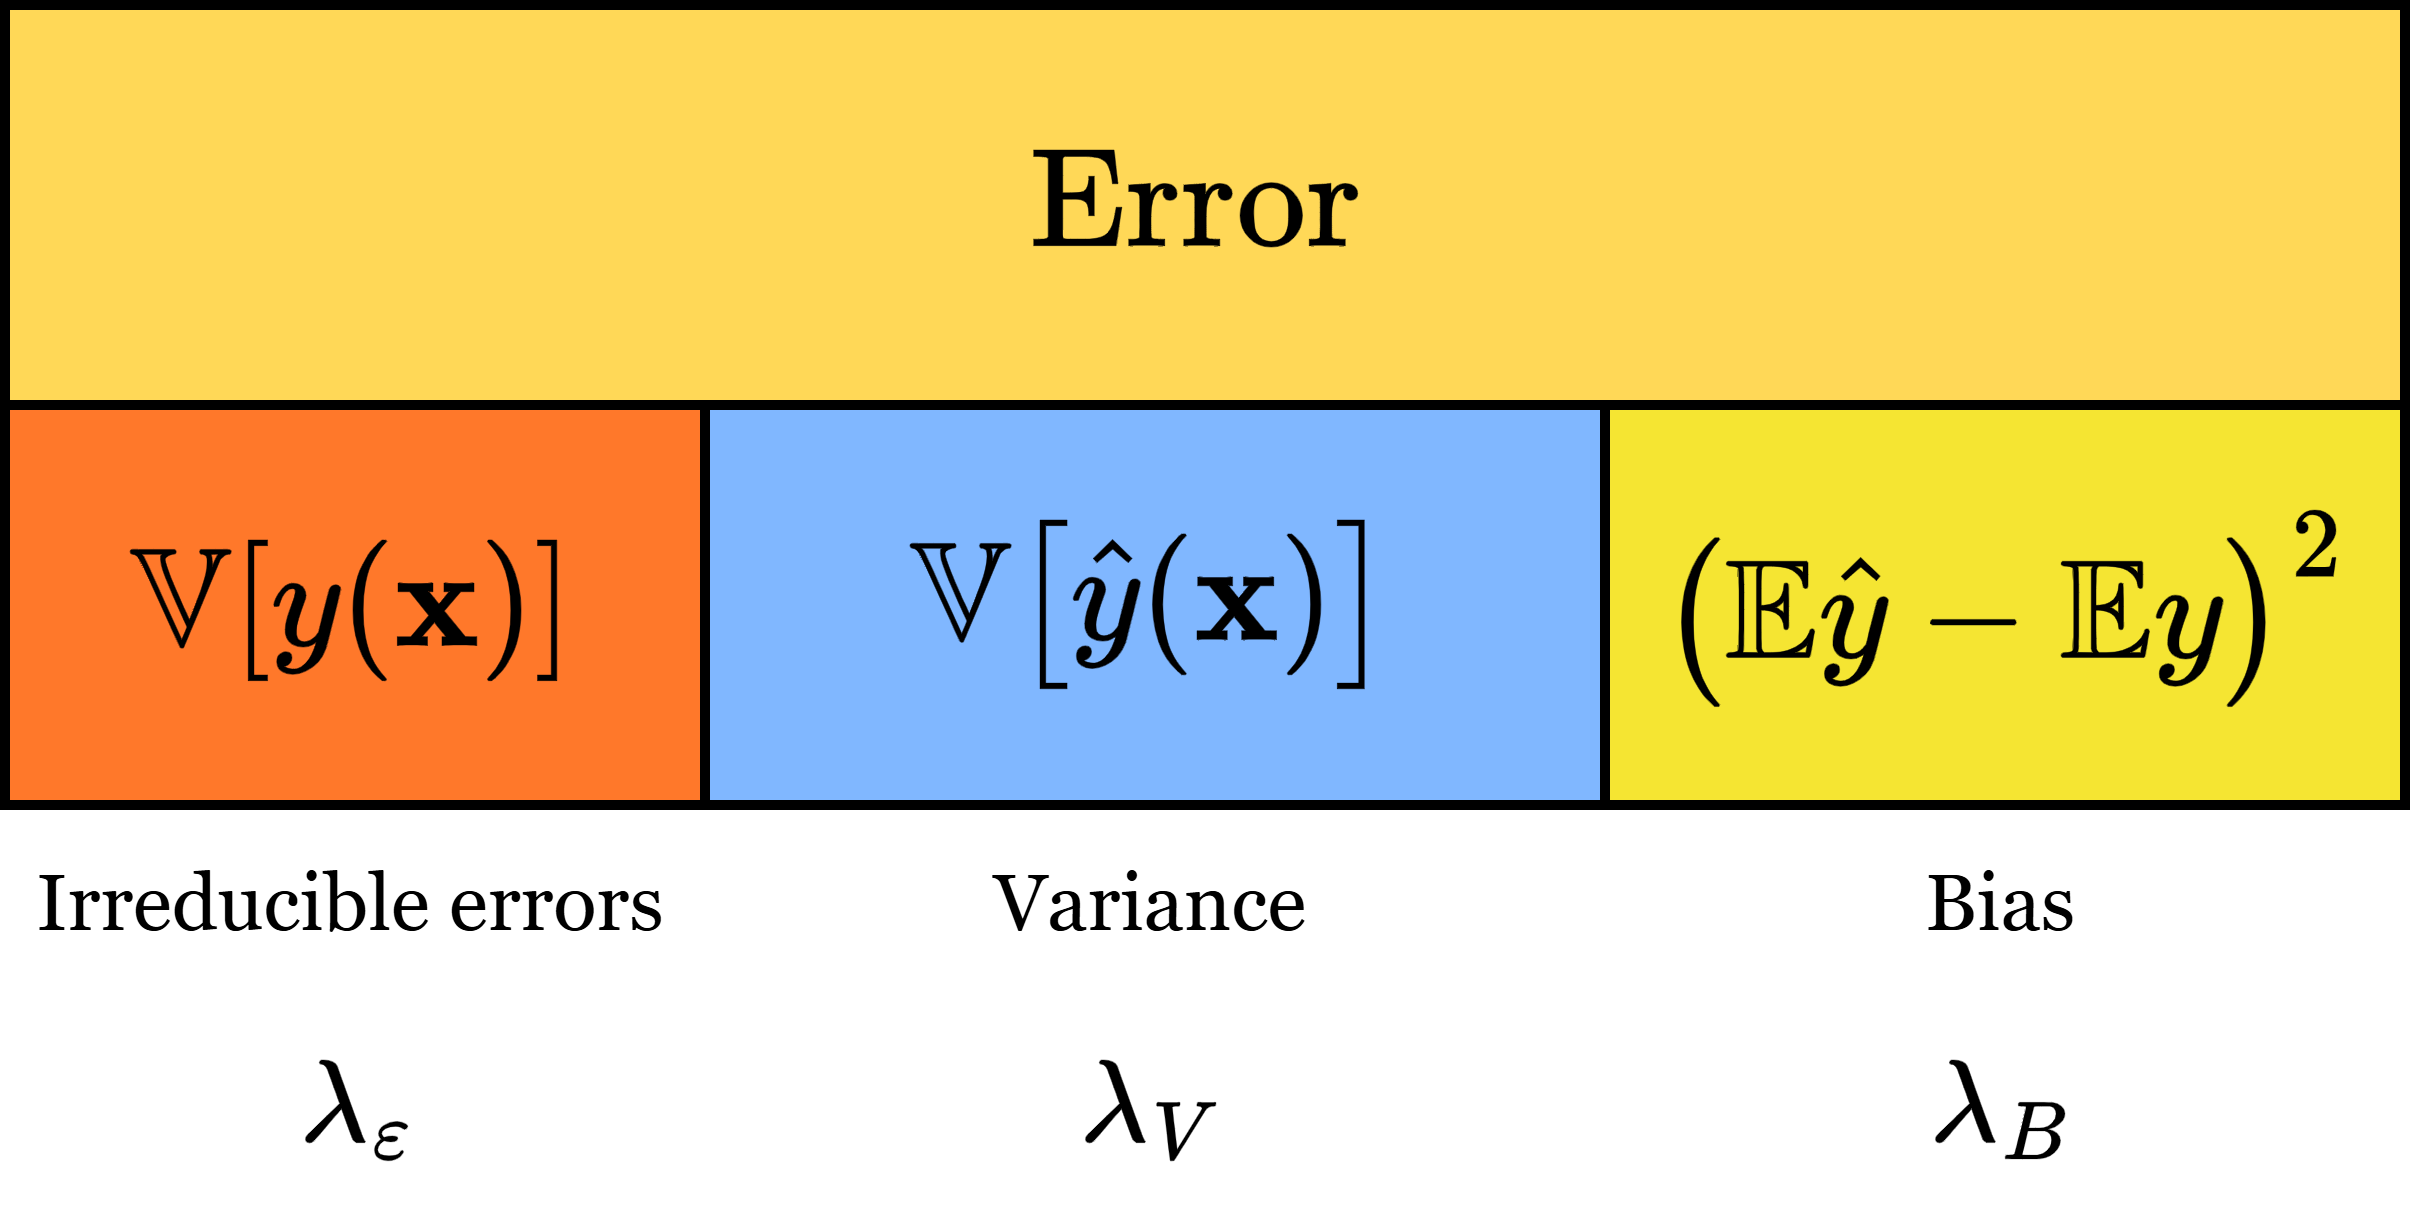
\includegraphics[width=0.5\textwidth]{error_decomposition.png}
  \caption{\textbf{Decomposition of the error term into 3 parts}. Respectively, the irreducible error $\mathbb{V}[y(\mathbf{x})]$, the variance (blue) and the bias (dark yellow). All of them are assumed to take up 100\% of the error observed in such composition. The proportion is included using the three coefficient $\lambda_{\epsilon},\lambda_{V},\lambda_{B}$ where $\lambda_{\epsilon}+\lambda_{V}+\lambda_{B}=1$.}
\end{SCfigure}

%\begin{figure}[htb]
%    \centering
%    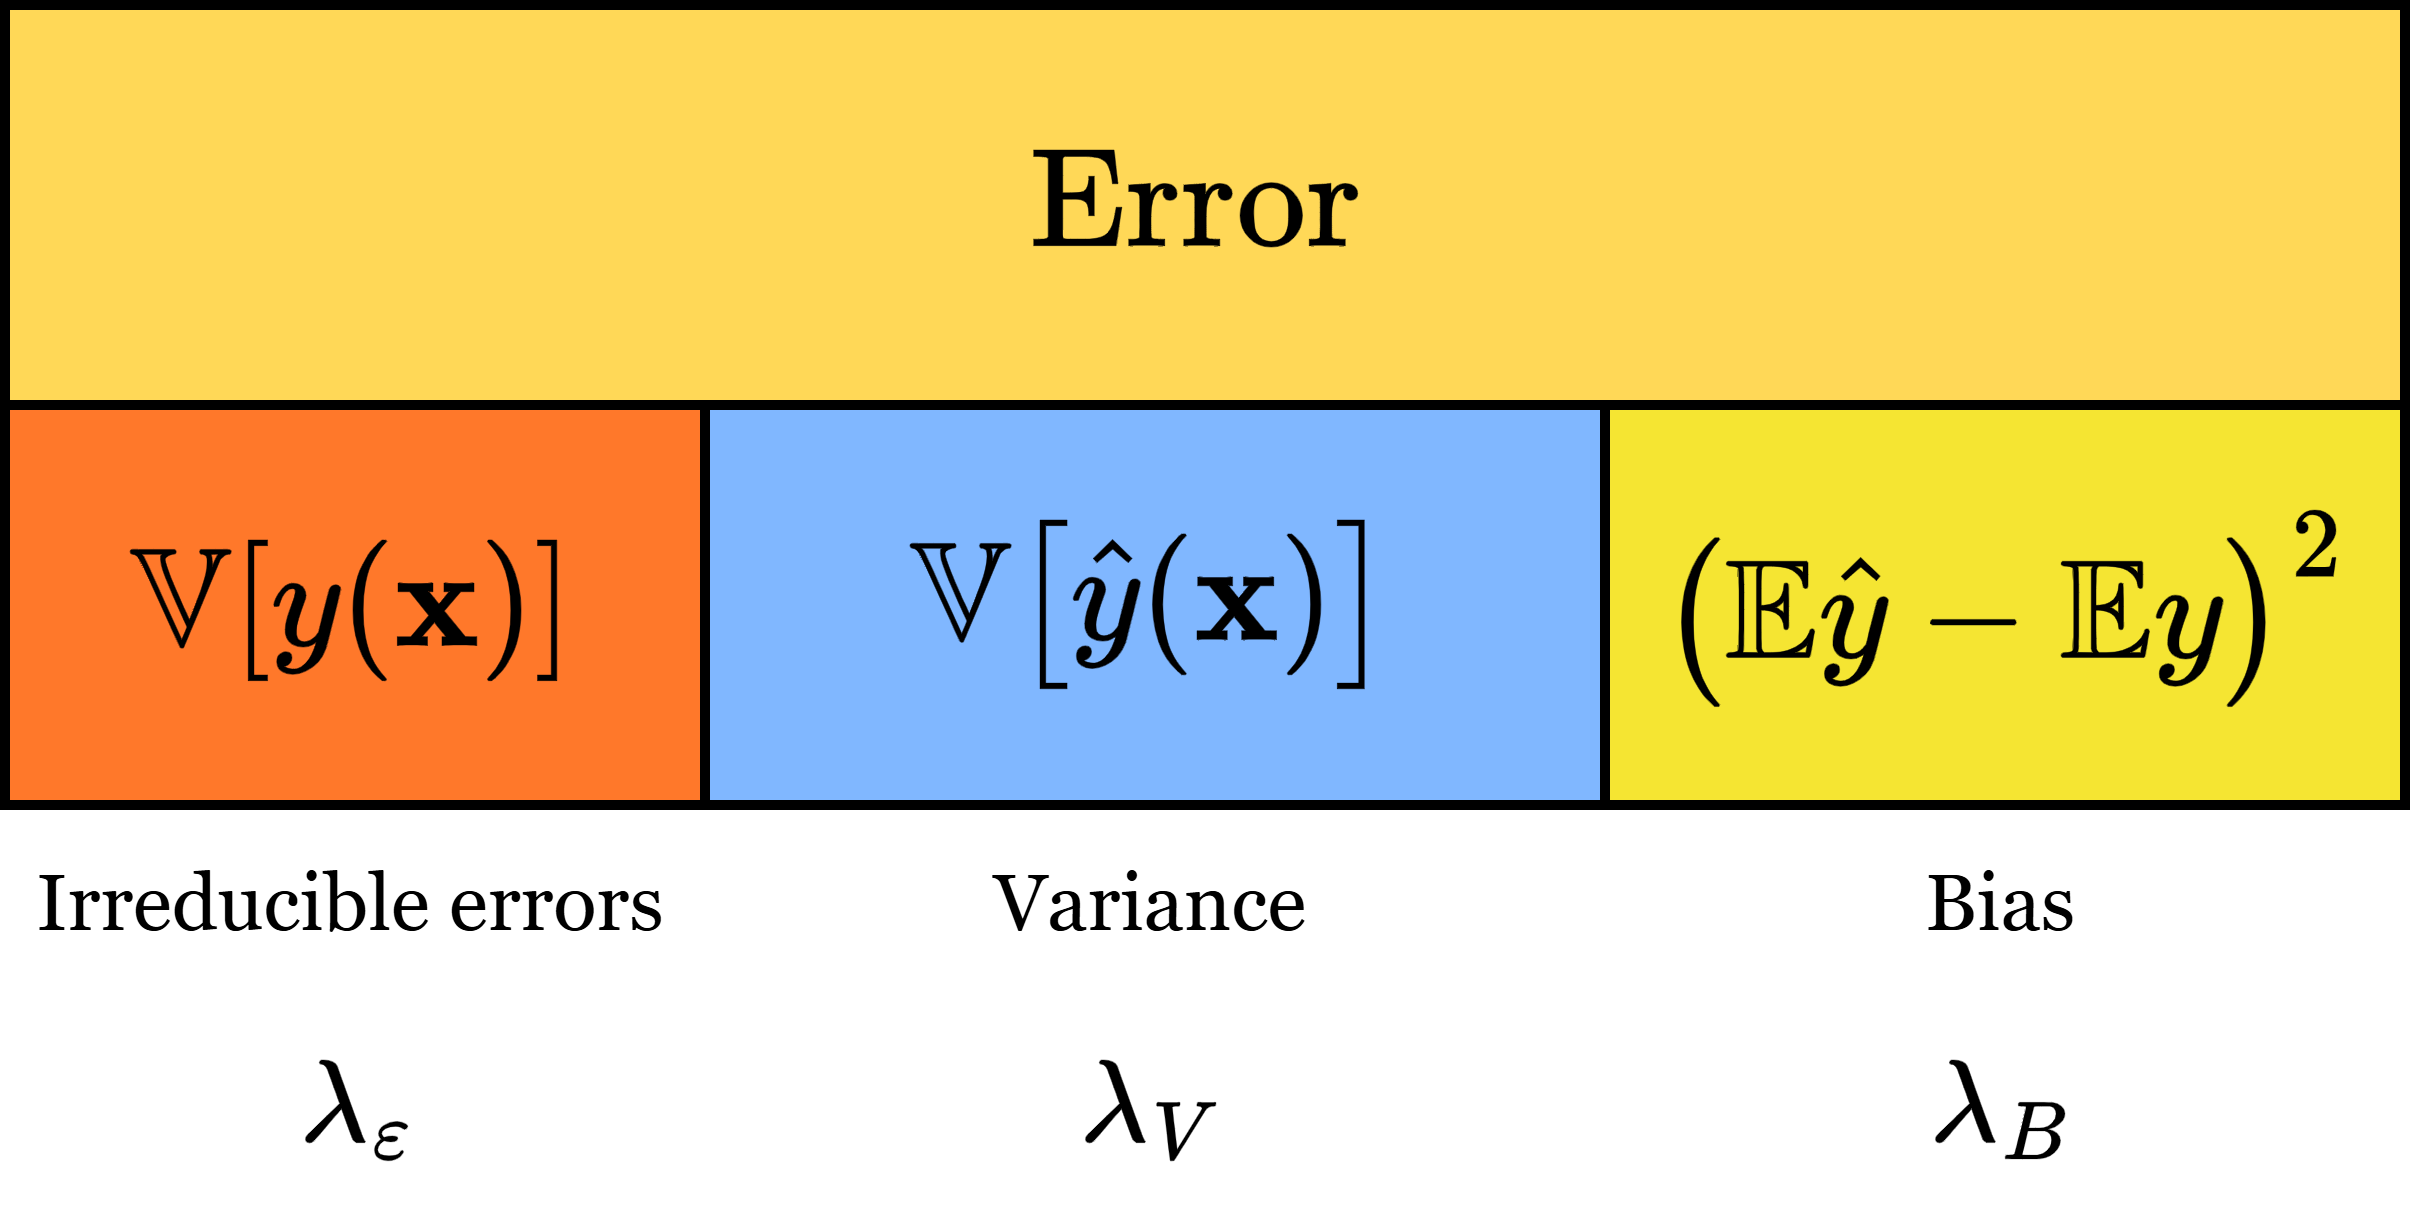
\includegraphics[width=0.4\textwidth]{error_decomposition.png}
%    \caption{\textbf{Decomposition of the error term into 3 parts}. Respectively, the irreducible error $\mathbb{V}[y(\mathbf{x})]$, the variance (blue) and the %bias (dark yellow). All of them are assumed to take up 100\% of the error observed in such composition. The proportion is included using the three coefficient %$\lambda_{\epsilon},\lambda_{V},\lambda_{B}$ where $\lambda_{\epsilon}+\lambda_{V}+\lambda_{B}=1$.}
%\end{figure}

The above decomposition principle is often expressed into a form where there exists the intrinsic noise \cite{brown2024biasvariance}: 
\begin{equation}
    \begin{split}
        \mathbb{E}_D \left[ \mathbb{E}_{xy} \left( y - \hat{f}(x) \right)^2 \right]
        &= 
         \mathbb{E}_x \left[ \left( y^* - \mathbb{E}_D[\hat{f}(x)] \right)^2 \right]
        + \mathbb{E}_x \left[ \mathbb{E}_D \left( \hat{f}(x) - \mathbb{E}_D[\hat{f}(x)] \right)^2 \right] \\
        &+ \mathbb{E}_{xy} \left[ \left( y - y^* \right)^2 \right]
    \end{split}
    \end{equation}
For simplicity of notation, we adopt the similar form in the standard case of \cite{adlam2020understandingdoubledescentrequires}: 
\begin{equation}
    \E \qa{\hat{y}(\bfx)-y(\bfx)}^2 = \pa{\E\hat{y}(\bfx) - \E y(\bfx)}^2 + \V\qa{\hat{y}(\bfx)} + \V\q{y(\bfx)}
\end{equation}
A main common theme of criticism toward bias-variance tradeoff is the fact that the decomposition is much more general, and intrinsic for the class of \textit{mean squared loss}. However, when considering the naturalness of an error measure and then its direct applicant, mean square error on real space of sufficient support and measure comes of as a very natural choice of an error measure, at least in consideration of the regression setting; for that, we then can also define classification as another top-layer above a regression's similar real continuous space, i.e. a decision layer. Furthermore, it can also be shown \cite{brown2024biasvariance,PfauBregmanDivergence} that it also holds for the class of Bregman divergence measure. 

In general, bias-variance is typically presented. In fact, one of the reason that it became the rule-of-thumb for ML practitioner, as well as generally statistical learning (\cite{lafon_understanding_2024} provides a quite rigorous treatment of bias-variance tradeoff in the section on statistical learning theory) solidify the trade-off as a particular model selection principle. Generally, this tradeoff can be summarized as followed: 
\begin{theorem}[Bias-variance tradeoff]
    For the expected loss of any given hypothesis $h$, the bias $\mathcal{B}(f,y)$ and variance $\mathcal{V}(f,y)$ is inversely proportional, that is, $\mathcal{B}(f,y)\propto \lambda^{-1} \mathcal{V}(f,y)$ for some proportionality $\lambda$ that may or may not be constant. In the most general case possible, $\lambda = -1$ on the entire error range. 
\end{theorem}

The tradeoff is then of inverse proportionality. Indeed, statistically, we have such tradeoff on a statistical framework in a more concrete sense. For the bias to increase, variance will increase, of which the criterion is inverse - we would like to have more bias but lower variance, according to such theory. 

There are problems regarding such stance. The main problem is that generally, the bias-variance measure does not totally match the overall decomposition structure. Even with irreducible errors, there are factors which make it to incorporate other error factors in for the decomposition, of which is inexplainable. There are also works, for example, \cite{domingos_unifeid_2000}, of which decompose the error to 
\begin{equation*}
        \begin{split}
            \mathrm{Error} & = \lambda_{1} \mathrm{Bias}(f,y) + \lambda_{2}\mathrm{Var}(f,y)+ \lambda_{3}\epsilon(\mathcal{D})\\ 
            & = \lambda_{1}\underbrace{\left\{ \mathbb{E}_{\mathcal{D}}[f(x;\mathcal{D})] , \mathbb{E}[y\mid x] \right\}}_{\text{bias term}} +\lambda_{2} \underbrace{\mathbb{E}_{\mathcal{D}} \left\{(f(x;\mathcal{D}), \mathbb{E}_{\mathcal{D}}[f(x;\mathcal{D})])\right\}}_{\text{variance term}} +\underbrace{\lambda_{3}\epsilon}_{\text{irreducible error}}
        \end{split}
\end{equation*}
of which the bias-variance-irreducible error are `fit' into the total error by three coefficients $\lambda_{1},\lambda_{2},\lambda_{3}$ instead. This does not only scale up the B-V-IE triplet, but also leaves out the inexplainable gap between the scaling, and the actual normal measure. 

The bias-variance decomposition and tradeoff is not general. Indeed, works, by \cite{6797087,sharma_bias-variance_2014,domingos_unifeid_2000,adlam2020understandingdoubledescentrequires,yang_rethinking_2020} and more all attempted to reconstruct and reformulate bias-variance, and it did leave out a picture of uncertainty regarding the concept. 

\subsection{Statistical learning theory perspective}
By statistical learning theory, we observed that there are plenty tradeoffs, most notably the empirical-generalization tradeoff, though we would have to clarify what those terms are. Furthermore, there is also what can be seen to be the analogue bias-variance tradeoff in such sense, is the \textit{approximation-estimation tradeoff} of statistical learning theory, though it must be clarified that they are strictly not the same, as seen from \cite{brown2024biasvariance}. 

Informally, the empirical-generalization tradeoff can be said to be the balancing act between achieving the true generalization and the empirical best. To achieve the generalization best, the empirical best, for finite hypothesis $\mathcal{H}$ (\cite{10.5555/2371238}), 
\begin{equation}
  \lim_{n\to \infty} \left[\underset{\mathcal{S}_{n}\sim \mathcal{D}^{m}}{\mathbb{E}}(\hat{R}_{\mathcal{S}(h)})\right]  = R(h), \quad h\in \mathcal{H}
\end{equation} 
This follows by the law of large number, and the statistical-probabilistic interpretation of the learning setting. However, the tradeoff is not straightforward - it is rather considered between, for example, the time-complexity, sample-space size, and generalization best's reach of the model. That is, for large the dataset is, the easier it is to get a sample space that represents more and more of the actual concept. However, in exchange, time-complexity increases, and thereby, the ergonomic aspect must be also considered. It is also concerned of the fact that the empirical best is not the same as even the generalization best, thereby, one will want their hypothesis class to extend. By doing this, they extend the outreach of the hypothesis class, however make it unstable under random, iterative process typically used to train such model to target. 

This is also noticed and formulated in the concept of approximation-estimation tradeoff. We refer to \cite{10.5555/2371238,lafon_understanding_2024} for some analysis and mentions. 

Let $\mathcal{H}$ be a family of functions mapping $\mathcal{X}\to\{1,-1\}$. This is the particular case of \textbf{binary classification}, in which can be straightforwardly extended to different tasks and loss functions. The \textit{excess error} of a hypothesis $h\in\mathcal{H}$, is the difference between its error $R(h)$ and the Bayes error $R^{*}$. This can be decomposed to be the following: 

\begin{equation}
    R(h) - R^{*} = \Big( R(h) - \inf_{h\in \mathcal{H}} R(h) \Big) + \Big( \inf_{h\in \mathcal{H}} R(h) - R^{*} \Big)
\end{equation}

The first bracket contains the \textbf{estimation error}, and the second bracket contains what is called the \textbf{approximation error}. The estimation error depends on the hypothesis $h$ selected. It measures the error of $h$ with respect to the infimum of the error achieved by hypotheses in $\mathcal{H}$, or that of the best-in-class hypothesis $h^{*}$ when that infimum is reached. The approximation error measures how well the Bayes error can be approximated using $\mathcal{H}$. It is a property of the hypothesis set $\mathcal{H}$, a measure of its richness. 

\subsection{Gradient descent on bias-variance decomposition}

While the interpretation of what the bias-variance tradeoff, the usual training-versus-test curve, and statistical learning consideration, another interesting aspect to consider (as well for double descent), is how bias-variance decomposition acts on gradient descent and its components. This claim is perhaps reinforced by the work of \cite{adlam2020understandingdoubledescentrequires} which indicates that different bias-variance decompositions effects differently on the total system mechanism. 

\begin{figure*}[htb]
    \centering
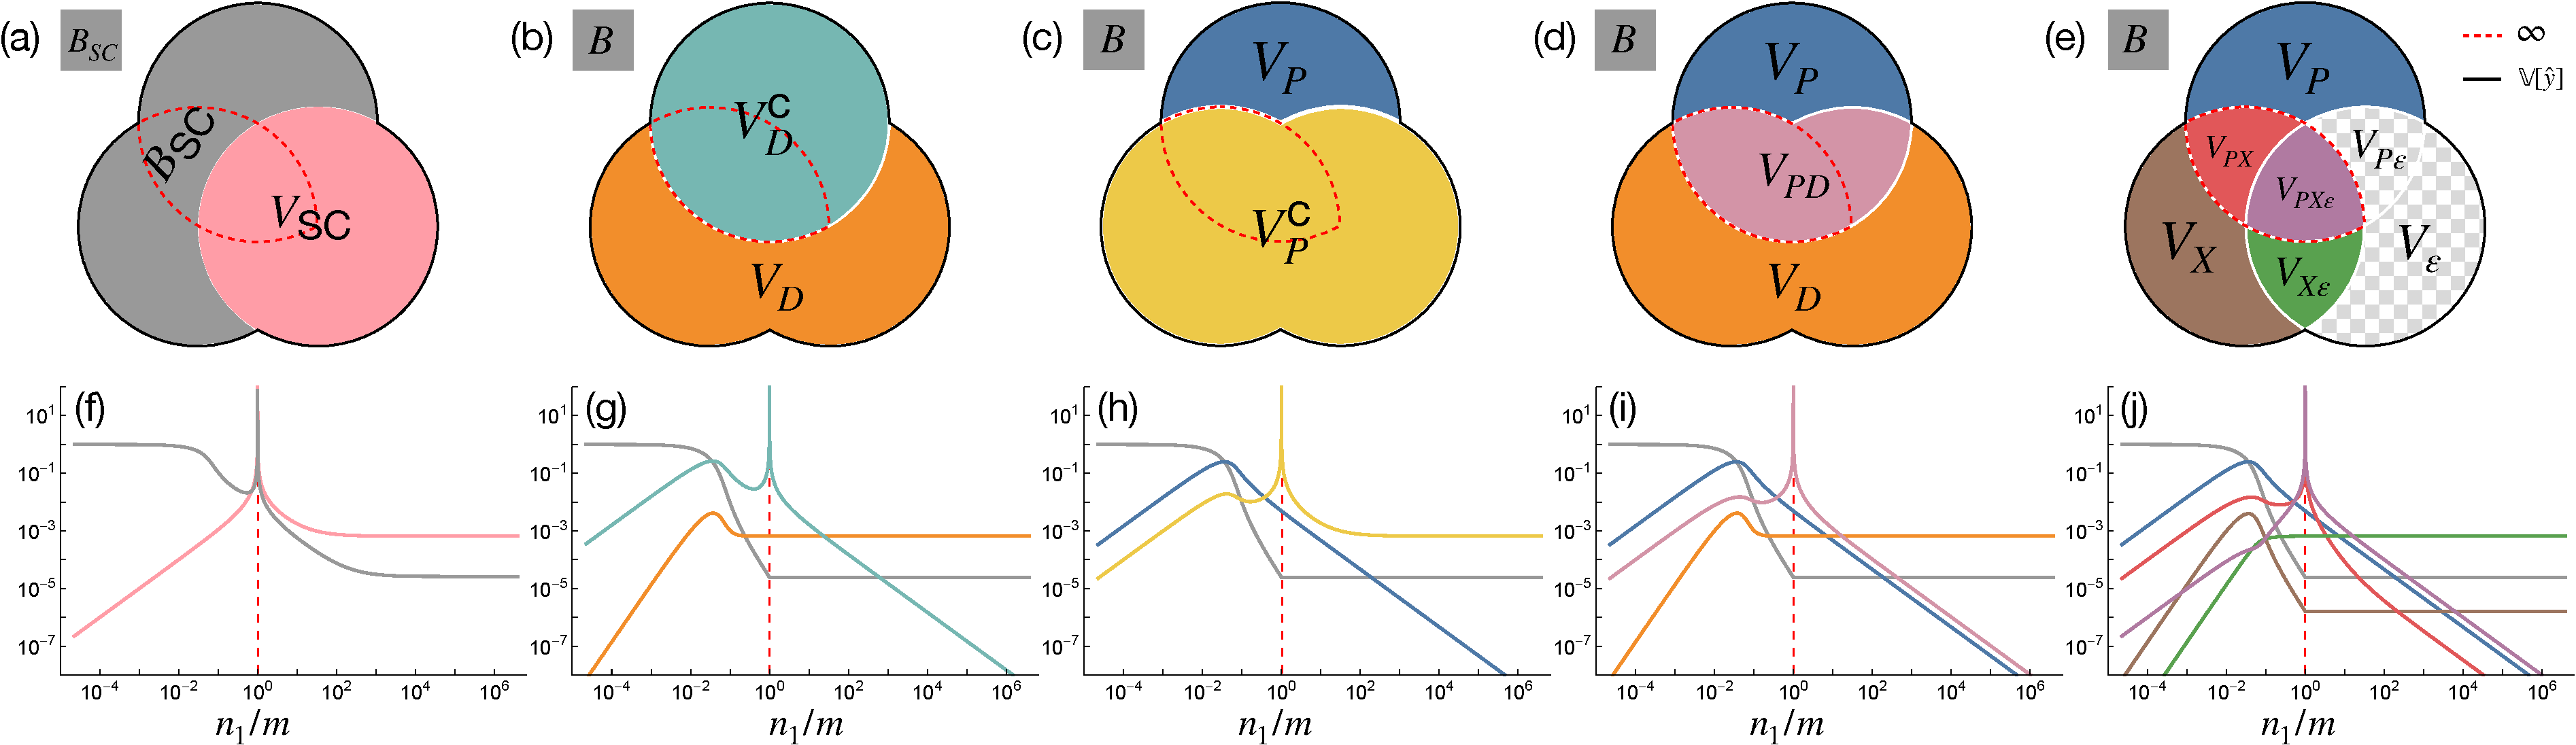
\includegraphics[width=\linewidth]{pdf/VennFig2.pdf}
\caption{(\textbf{a-e) The different bias-variance decompositions.} (f-j) Corresponding theoretical predictions for $\gamma =0$, $\phi=1/16$ and $\fs = \tanh$ with $\text{SNR} = 100$ as the model capacity varies across the interpolation threshold (dashed red). (a,f) The semi-classical decomposition of~\cite{hastie2019surprises,mei2019generalization} has a nonmonotonic and divergent bias term, conflicting with standard definitions of the bias. (b,g) The decomposition of~\cite{neal2018modern} utilizing the law of total variance interprets the diverging term $V_D^\textsc{c}$ as ``variance due to optimization''. (c,h) An alternative application of the law of total variance suggests the opposite, \emph{i.e.} the diverging term $V_P^\textsc{c}$ comes from ``variance due to sampling''. (d,i) A bivariate symmetric decomposition of the variance resolves this ambiguity and shows that the diverging term is actually $V_{PD}$, \emph{i.e.} ``the variance explained by the parameters and data together beyond what they explain individually.'' (e,j) A trivariate symmetric decomposition reveals that the divergence comes from two terms, $V_{PX}$ and $V_{PX\bfe}$ (outlined in dashed red), and shows that label noise exacerbates but does not cause double descent. Since $V_\e=V_{P\e}=0$, they are not shown in (j). Taken from \cite{adlam2020understandingdoubledescentrequires}}
\label{fig:venn_variance}
\end{figure*}

The main term of a gradient descent algorithm is the gradient of the loss function $\mathcal{L}(h(x),y)$. For the hypothesis $h$, the number of instances supplied denoted by $k$ has three main cases: $k=1$ for stochastic descent, $k\in (1,m)$ for batch gradient descent, and $k=m$ for standard gradient descent, for a given space of $m$ samples. The gradient in such case is calculated using the empirical risk on $m$ size, that is: 
\begin{equation}
    \mathcal{L}_{k}(h(x),y) = \hat{R}_{S[k]}(h) = \frac{1}{k} \sum^{k}_{i=1} \ell(h(x_{i}),y_{i})
\end{equation}
We use the classical bias-variance tradeoff at first. Since the gradient is a linear operator, we have: 
\begin{equation}
    \begin{split}
        \nabla_{k}(\mathcal{L}) &= \nabla_{k}\left(\pa{\E\hat{y}(\bfx) - \E y(\bfx)}^2 + \V\qa{\hat{y}(\bfx)} + \V\q{y(\bfx)}\right)\\
        & = \nabla_{k}\left( \E\left[\hat{y}(\bfx)\right] - \E\left[y(\bfx)\right] \right)^2 + \nabla_{k}\V\left[\hat{y}(\bfx)\right] + \nabla_{k}\V\left[y(\bfx)\right] \\
        & = \nabla_{k}\left( \E\left[\hat{y}(\bfx)\right] - \E\left[y(\bfx)\right] \right)^2 + \nabla_{k}\V\left[y(\bfx)\right]
    \end{split}
\end{equation}
This effectively decompose the gradient into three parts that influence the overall gradient calculation. Because $\nabla_{k}\V\left[y(\bfx)\right]$ calculates the gradient of irreducible error, which is supposed to be constant of the sample space, it is then equal $0$. Suppose a sample $\mathbf{x}_{k}$ of size $km$, of partition $k$. Hence, we have gradient descent based on $k$th run over the entire dataset, permuted. Then, the loss function calculates in the form 
\begin{equation}
  \nabla_{k,n}(\mathcal{L}) = \nabla_{k,n}\left[ \frac{1}{n}\sum_{i\leq n} \hat{y}(x_{kn+i})  - \frac{1}{n}\sum_{i\leq n} y(x_{kn+i}) \right]^{2} + \nabla_{k,n} \left[ \frac{1}{n}\sum_{i=1}^n y(x_i)^2 - \left( \frac{1}{n}\sum_{i=1}^n y(x_i) \right)^2 \right]
\end{equation}
The indices is now changed to $(k,n)$ for $m/k=n$ as the $i$th partitioned, ordered run, thereby $kn+i$ runs for the index. If we assume a simplified structure $\theta_{t}$ of parameters $y(x_{i})$ depends on, we can reduce it further.  

\begin{align}
\nabla_{k,n}(\mathcal{L})
&= 2\left(\frac{1}{n}\sum_{i\le n}\hat{y}(x_{kn+i}) - \frac{1}{n}\sum_{i\le n}y(x_{kn+i})\right)
   \left(\frac{1}{n}\sum_{i\le n}\nabla_k\hat{y}(x_{kn+i}) - \frac{1}{n}\sum_{i\le n}\nabla_k y(x_{kn+i})\right) \\
&+ \frac{2}{n}\sum_{i=1}^n y(x_i)\nabla_k y(x_i)
   - \frac{2}{n^2}\left(\sum_{i=1}^n y(x_i)\right)\left(\sum_{i=1}^n \nabla_k y(x_i)\right)
\end{align}

\section{Double descent}

Nevertheless, of bias-variance and the analogous statistical learning theory concept, the target is the same. It is the dilemma of which is presented in \textbf{Occam's razor}, for choosing the sufficient model of good complexity, or bias, for tradeoff of its generalization ability, or variance. Then there must exist a sweet spot between the axis of bias and variance, since they are as exhibited above inversely proportional to each other. However, double descent seemingly broke the status quo, and insists on an interesting phenomenon - under the same setting, if we `crank' the complexity high enough, we will then reach a point then called the \textbf{interpolation threshold}, such that the trend reverse and the error rate, instead of being theorized to go up, goes down to a certain line of lower bound. 

The first identification of the double descent phenomena dated back to the paper of Belkin - \cite{belkin_reconciling_2019}, in which the title is literally "reconciling" modern machine learning practice and the bias-variance tradeoff. In modern machine learning practice, or state-of-the-art developments, models are now bigger than ever. If to notice, we will see that currently models are inherently large, for example, a normal large language model will have from 900 millions (900M) to a few billions, for example 10 billions (10B) parameters. That is not taking into account the overall dynamics and structure of the model, which dictates the operating range and efficiency of the model itself. These model, based on the neural network architecture are somewhat trained to exactly fit (or interpolate) the data, almost certainly so that it turn from a prediction setting to an estimation setting. By statistical learning theory, this would be considered overfitting, and yet, they often obtain very high accuracy on test data.

\begin{figure}[htb]
    \centering
    \begin{tabular}{cc}
    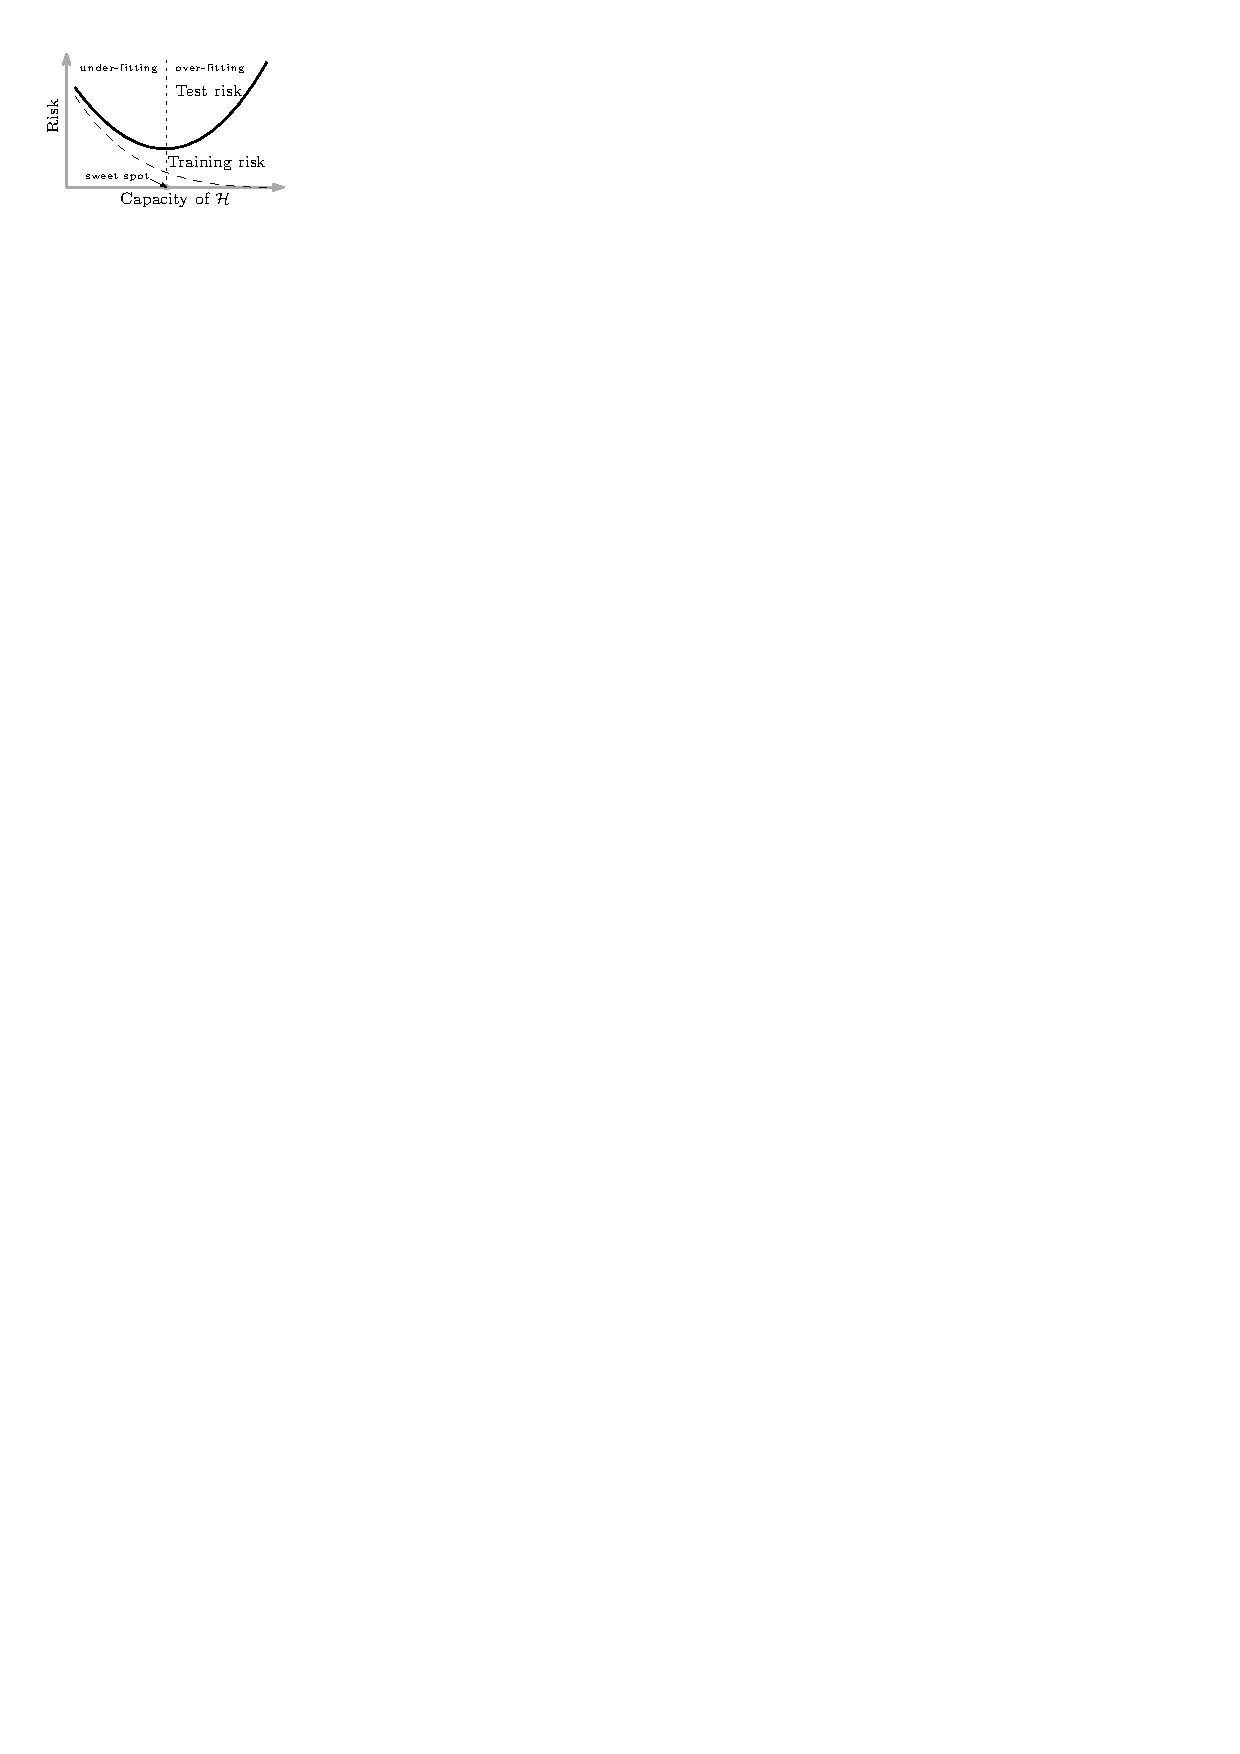
\includegraphics[height=0.15\textheight]{pdf/u-shaped.pdf} &
    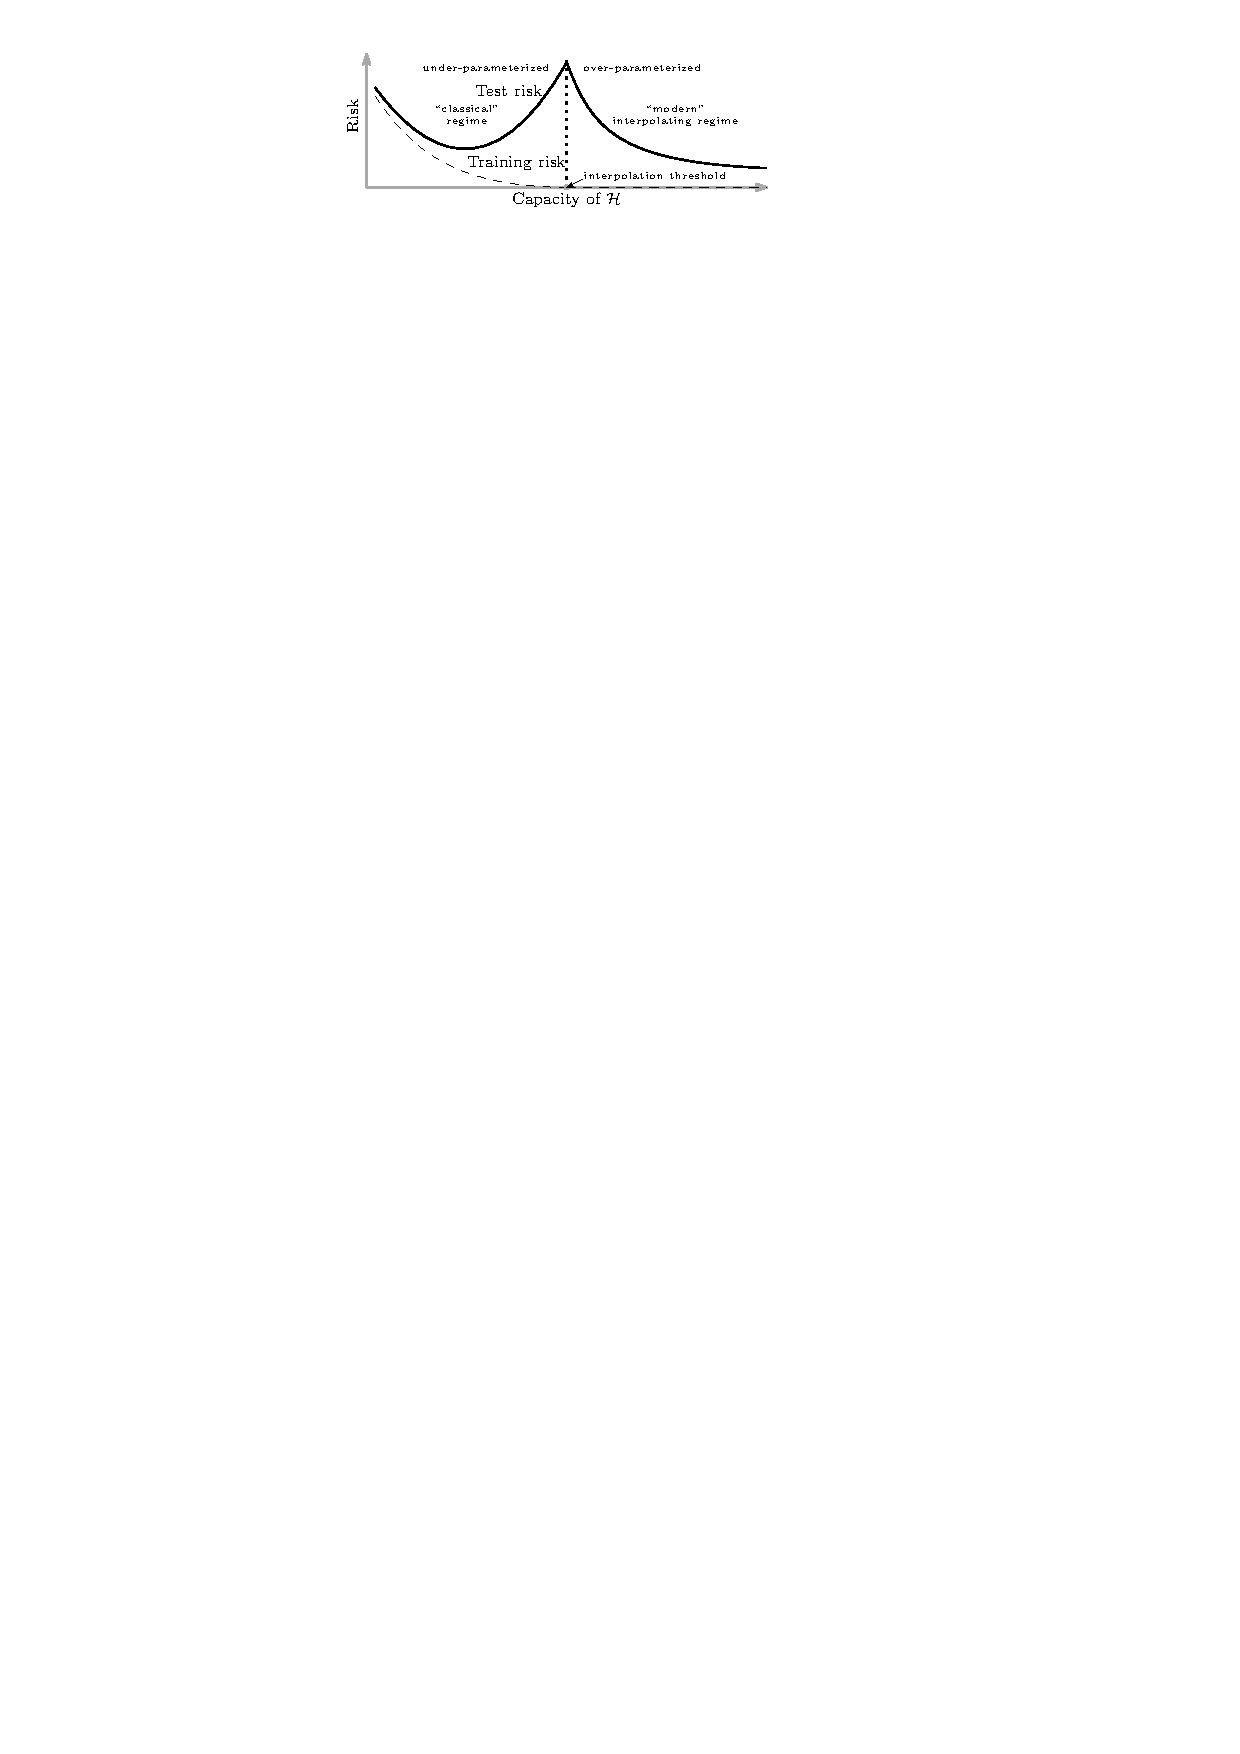
\includegraphics[height=0.15\textheight]{pdf/doubledescent.pdf} \\
    {\bf (a)} & {\bf (b)}
    \end{tabular}
    \caption{{\bf Curves for training risk (dashed line) and test risk (solid line).}
      ({\bf a}) The classical \emph{U-shaped risk curve} arising from the bias-variance trade-off.
      ({\bf b}) The \emph{double descent risk curve}, which incorporates the U-shaped risk curve (i.e., the ``classical'' regime) together with the observed behaviour from using high capacity function classes (i.e., the ``modern'' interpolating regime), separated by the interpolation threshold.
      The predictors to the right of the interpolation threshold have zero training risk. Reproduced from \cite{belkin_reconciling_2019}.}
    \label{fig:double-descent}
\end{figure}

The main finding that Belkin found is a pattern for how the apparent performance on unseen data depends on model capacity and the mechanism underlying the emergence of double descent. When function class capacity is below the "interpolation threshold", learned predictors exhibit the classical $U$-shaped curve from Figure~\ref{fig:double-descent}. The `modern' interpolating regime marks the opposite trend to the right, where the risk starts to decrease up to a lower bound, which then can be called the \textit{optimal descent bound}. 

\blockquote[\cite{belkin_reconciling_2019}]{The bottom of the $U$ is achieved at the sweet spot which balances the fit to the training data and the susceptibility to over-fitting:
to the left of the sweet spot, predictors are under-fit, and immediately to the right, predictors are over-fit.
When we increase the function class capacity high enough (e.g., by increasing the number of features or the size of the neural network architecture), the learned predictors achieve (near) perfect fits to the training data---i.e., interpolation.
Although the learned predictors obtained at the interpolation threshold typically have high risk, we show that increasing the function class capacity beyond this point leads to decreasing risk, typically going below the risk achieved at the sweet spot in the ``classical'' regime.}

Another prominent result to look at is \cite{nakkiran_deep_2019}, on the double descent of deep learning models. This is the first step toward identifying double descent to be perhaps, universal. 

\begin{figure}[htb]
    \centering
    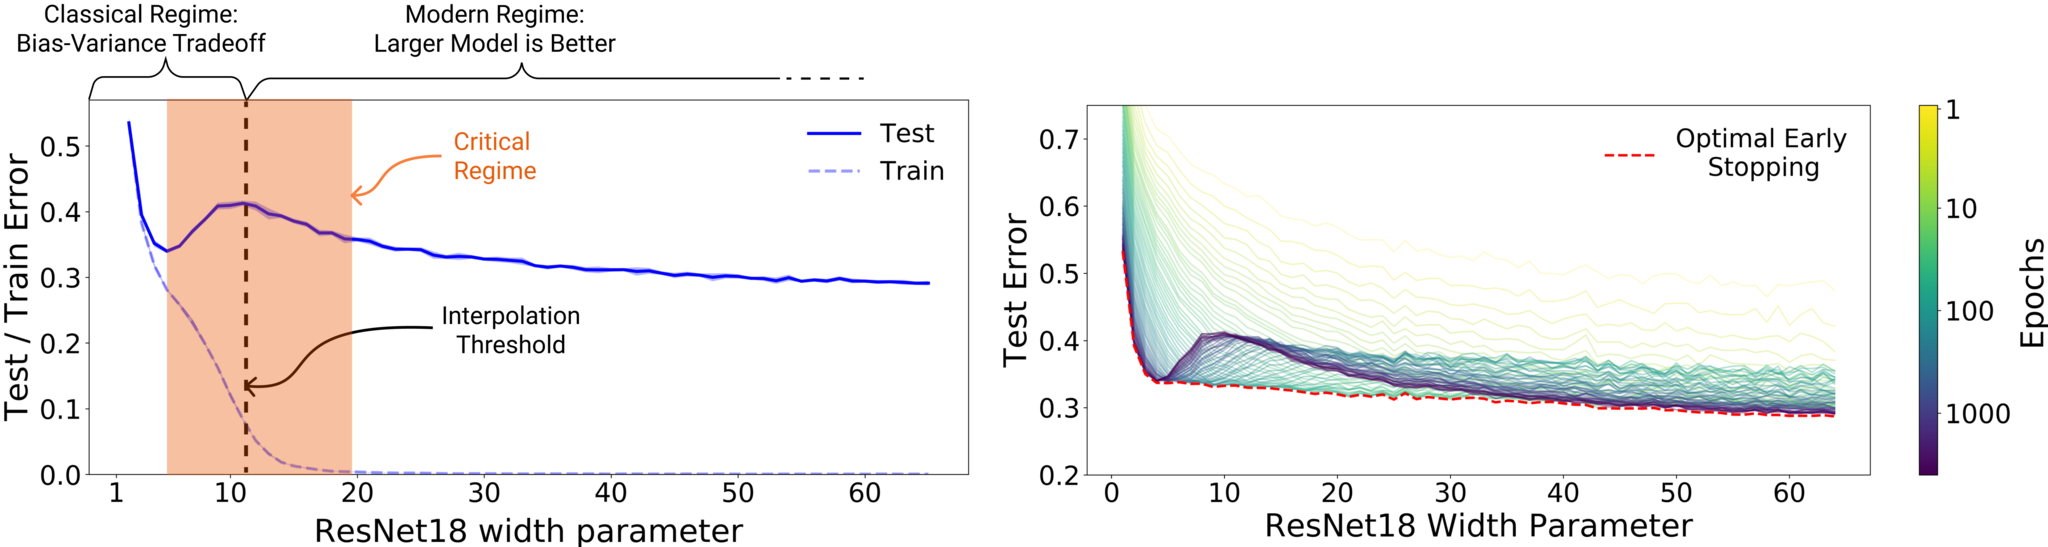
\includegraphics[width=1.05\textwidth]{errorvscomplexity.png}
    \caption{{\bf Left:} Train and test error as a function of model size,
    for ResNet18s of varying width 
    on CIFAR-10 with 15\% label noise.
    %In the under-parameterized regime, test error follows
    %the behavior predicted by classical statistical learning theory, but in the overparameterized regime (once training error is approximately zero),  the test error undergoes a ``second descent'' and decreases as model size increases. The shaded region represents the critically parameterized regime where the transition from under- to over-parameterization occurs. 
    {\bf Right:}
    Test error, shown for varying train epochs.
    %The dashed red line shows that with optimal early stopping double descent is not observed.
    % All models are ResNet18s of varying width,
    % trained on CIFAR10 with 15\% label noise
    All models trained using Adam for 4K epochs.
    %, and plotting means and standard-deviations from 5 trials with random network initialization.
    The largest model (width $64$) corresponds to standard ResNet18. Resued from \cite{nakkiran_deep_2019}.
    %    \ptodo{point out that interpolation point for second plot is plotted in the ocean plot}
    }
    \label{fig:errorvscomplexity}
\end{figure}

\begin{figure}[htb]
\centering
\begin{minipage}{.512\textwidth}
  \centering
  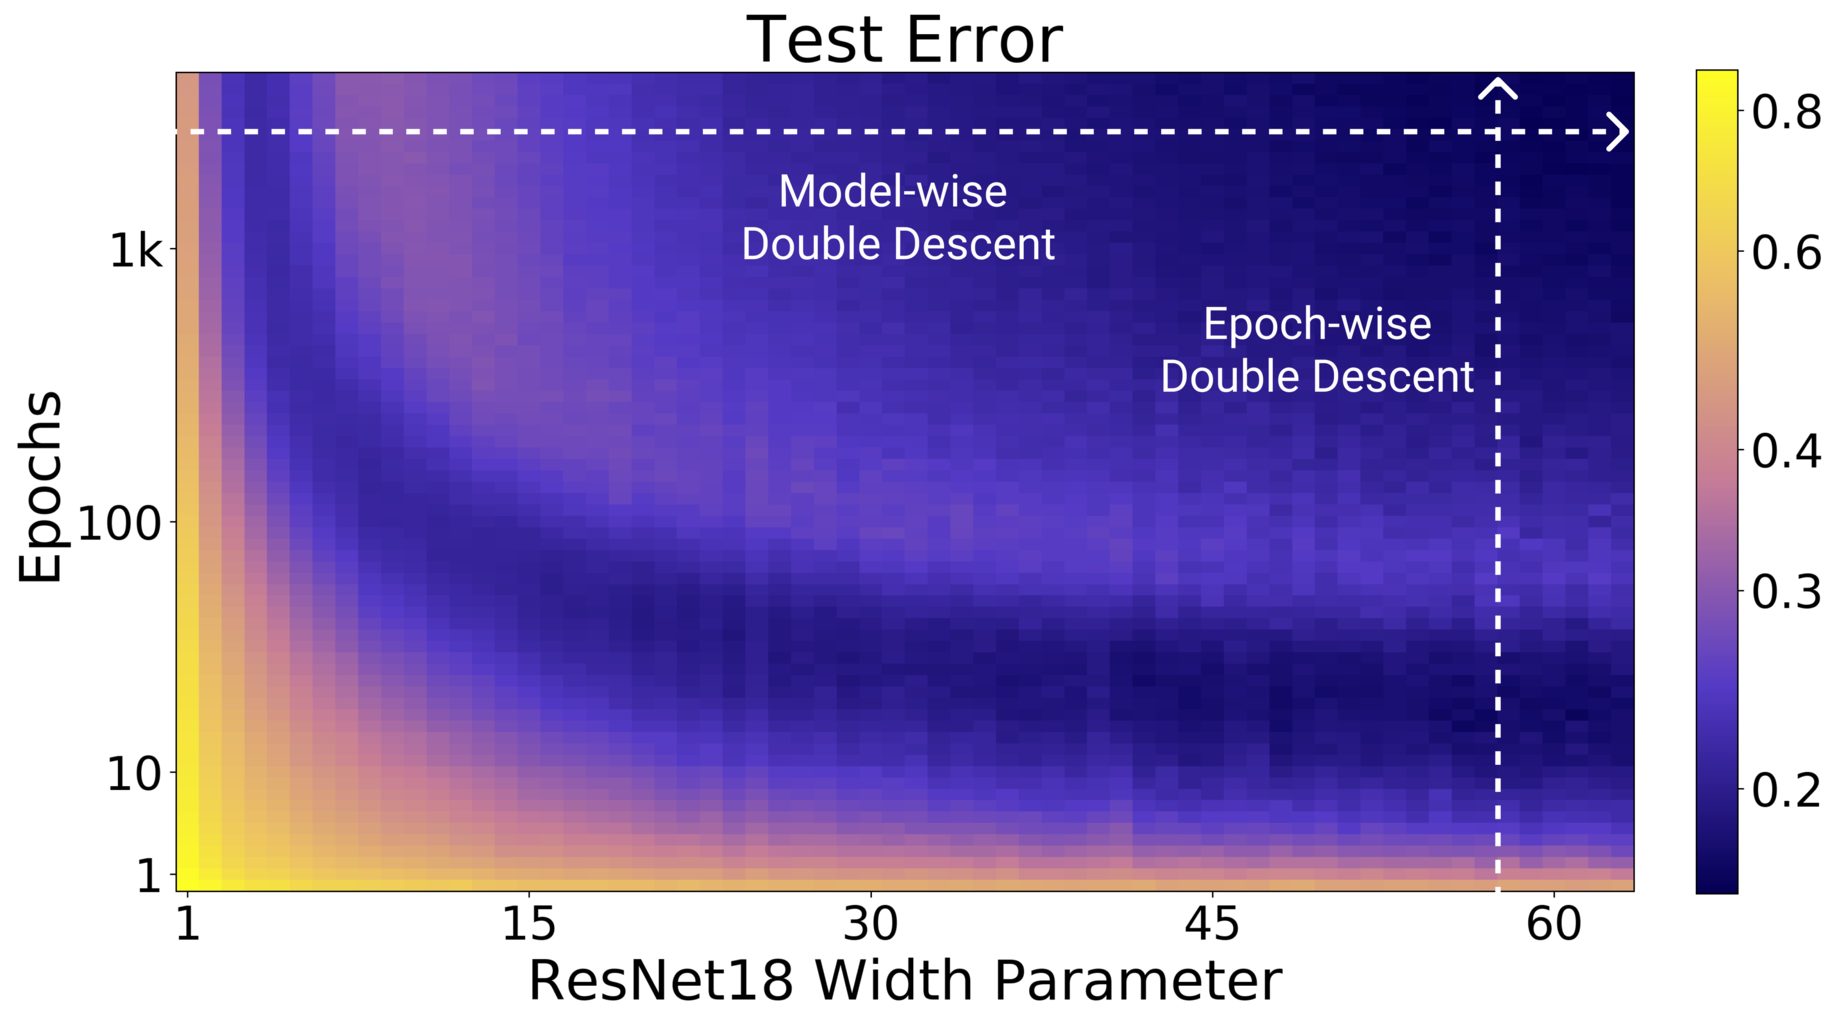
\includegraphics[width=1\textwidth]{Intro-ocean-test.png}
\end{minipage}%
\begin{minipage}{.488\textwidth}
  \centering
  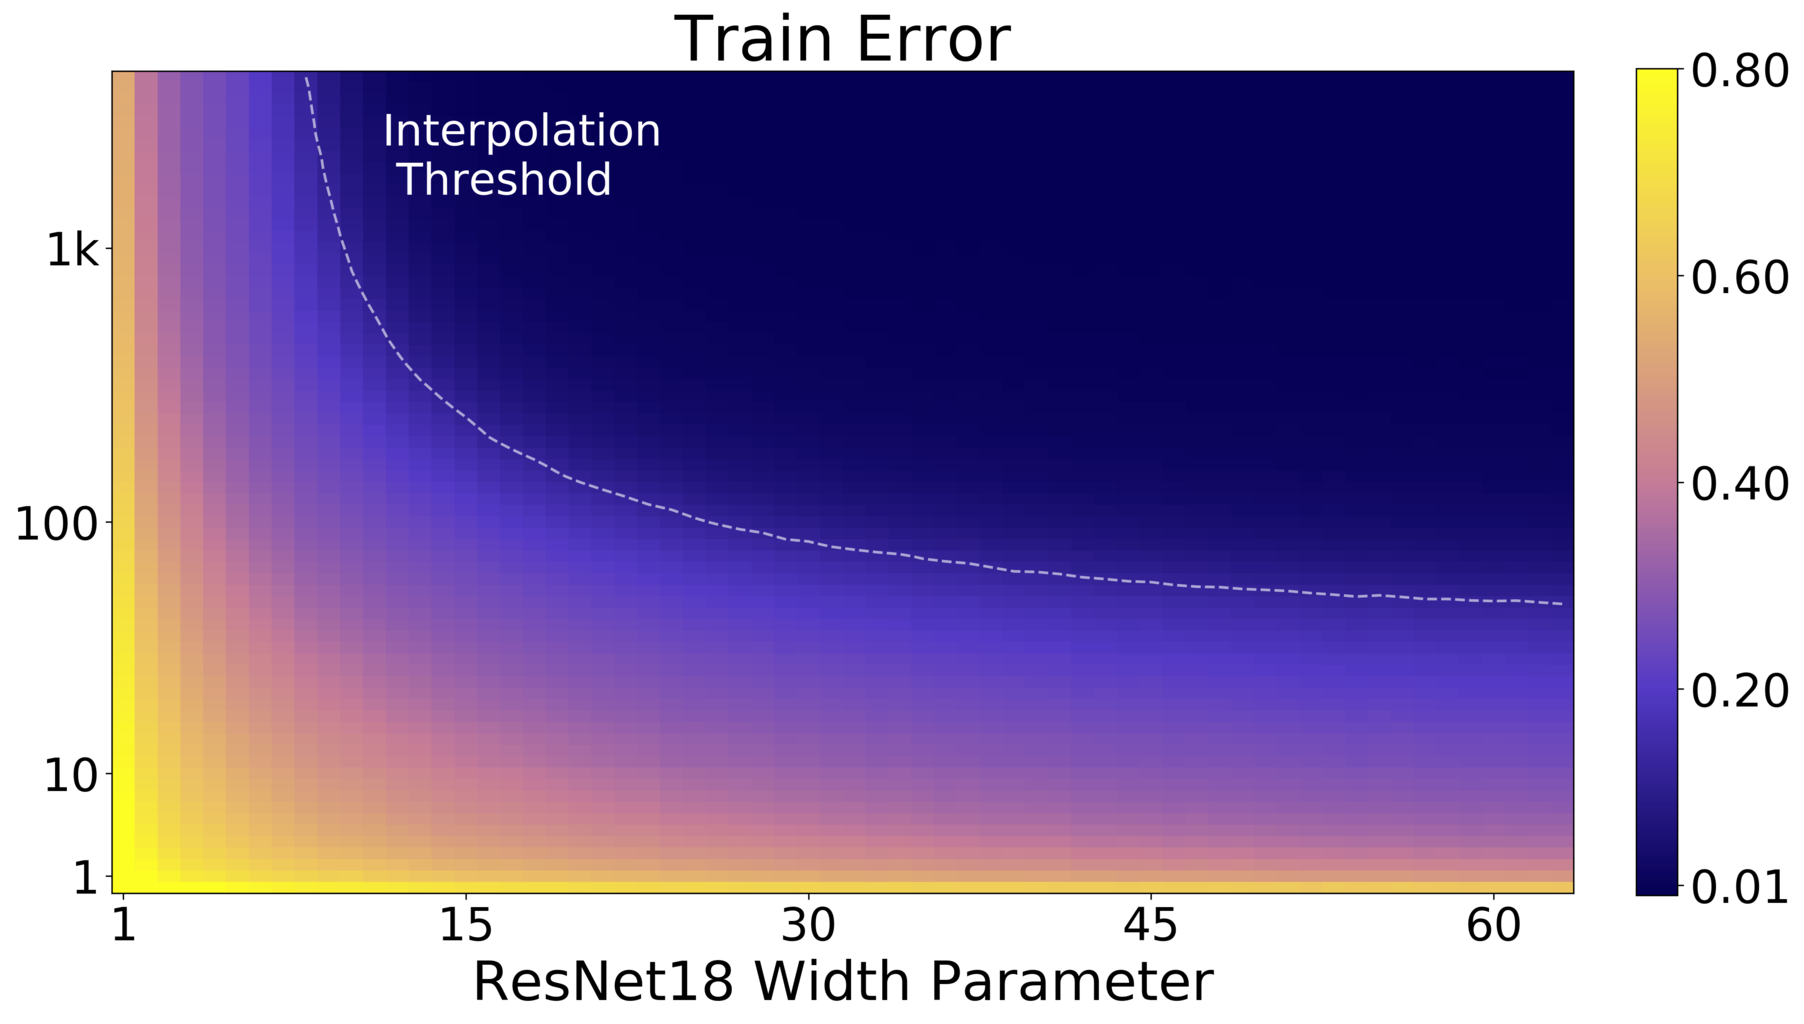
\includegraphics[width=1\textwidth]{Rn-cifar10-p15-adam-aug-train.png}
\end{minipage}
\caption{{\bf Left:} Test error as a function of model size and train epochs. The horizontal line corresponds to model-wise double descent--varying model size while training for as long as possible.
The vertical line corresponds to epoch-wise double descent,
with test error undergoing double-descent as train time increases.
{\bf Right} Train error of the corresponding models.
All models are Resnet18s trained on CIFAR-10 with 15\% label noise,
data-augmentation, and Adam for up to 4K epochs. Reused from \cite{nakkiran_deep_2019}}
\label{fig:unified}
\end{figure}

They define \emph{effective model complexity} of $\mathcal{T}$ (w.r.t. distribution $\mathcal D$) to be the maximum number of samples $n$ on which $\mathcal{T}$ achieves on average $\approx 0$ \emph{training error}. This is an entirely empirical definition, similarly per definition as VC-dimension. 

\newcommand{\EMC}{\mathrm{EMC}}
\begin{definition}[Effective Model Complexity]
The \emph{Effective Model Complexity} (EMC) of a training procedure $\cT$, with respect to distribution $\cD$ and parameter $\epsilon>0$,
is defined as:
\begin{align*}
    \EMC_{\cD,\eps}(\cT)
    :=  \max \left\{n ~|~ \E_{S \sim \cD^n}[ \mathrm{Error}_S( \cT( S )  ) ] \leq \eps \right\}
    \end{align*}
    where $\mathrm{Error}_S(M)$ is the mean error of model $M$ on train samples $S$.
\end{definition}

Using this definition, their main hypothesis can then be stated as the following three-fold regions:

\begin{hypothesis}[Generalized Double Descent hypothesis, informal] \label{hyp:informaldd}
For any natural data distribution $\cD$, neural-network-based training procedure $\cT$, and small $\epsilon>0$,
if we consider the task of predicting labels based on  $n$ samples from $\cD$ then:
\begin{description}
    \item[Under-parameterized regime.]  If~$\EMC_{\cD,\epsilon}(\cT)$ is sufficiently smaller than $n$, any perturbation of $\cT$ that increases its effective complexity will decrease the test error.
    \item[Over-parameterized regime.] If $\EMC_{\cD,\epsilon}(\cT)$ is sufficiently larger than $n$,
    any perturbation of $\cT$ that increases its effective complexity will decrease the test error.
    
    \item[Critically parameterized regime.] If $\EMC_{\cD,\epsilon}(\cT) \approx n$, then
    a perturbation of $\cT$ that increases its effective complexity
    might decrease {\bf or increase} the test error.
\end{description}
\end{hypothesis}

It is to notice that this definition is also only observational. By that, it only outlines the specific region of interest where the paradigm shift is identified through experimental results. It has no effective predictive power, or rather descriptive power more than setting up hypothesis with respect to the effective model complexity, and some arbitrary perturbation. \cite{nakkiran_deep_2019} also noticed this difficulty in providing a theoretical definition and theorem regarding such hypothesis, as said in their manuscript. The existence of the critical regime is also not defined. 

The behaviour itself has been particularly investigated, in certain settings. For example, before \cite{belkin_reconciling_2019}, \cite{advani2017highdimensionaldynamicsgeneralizationerror} investigated the generalization error in neural networks of high-dimensional measure. Of such, various behaviours that bear similarity to double descent can be observed. \cite{belkin2018understanddeeplearningneed} expanded on his previous research on the particular subset of kernel learning models, providing a theoretical analysis of specifically the Laplacian kernel on standard neural network. \cite{mei2020generalizationerrorrandomfeatures} investigated random feature regression in such regard, and also found similar results. 

The fact that double descent is not well-defined itself is a problem on its own. Up to the author's knowledge, there has been no effective definition or given description that outlines specifically how double descent can be structured. Instability in reproducing experiments and the effective range of the phenomena remains a question on its own. 
\clearpage
\section{Pre-analysis of double descent}
Preliminary sections and historical remark on the problem, both bias-variance and double descent hinted at a potential deadlock in resolving such it. Conflicting notions and reports aid into the confusion of such topic more than can be normally observed, and the anomalous behaviours in some researches (for example, in \cite{shi2024homophilymodulatesdoubledescent}, we received that in GNN, there exists no trace of double descent) makes it even harder. As such, both the status of bias-variance being false, albeit in a given range only, and double descent in masking certain behaviours of the modelling process, have taken a mysterious stance in the modern machine learning community. 

While discovering the double descent phenomena, it also exposes theoretical concepts that are not organized or formalized, portions of the theory and empirical observations that are within conflict of each others, issues with definitions, theorems, and interpretation of them. Those problems would then ultimately hinder further research in such direction, as well as broader theoretical requirement of the theory of machine learning, and specifically to a larger and more complex system of deep learning. 
\subsection{Model complexity}
The notion of model complexity can be said to be often not so well-defined. There are attempts by \cite{hu2021modelcomplexitydeeplearning,luo2024investigatingimpactmodelcomplexity,barceló2020modelinterpretabilitylenscomputational,Molnar_2020,janik2021complexitydeepneuralnetworks}. The problem of model complexity is not so apparent until the inherent complex nature of models, typically in deep learning models (based on the MLP architecture) is observed to cannot be treated in similar way as classical models. In \cite{hu2021modelcomplexitydeeplearning}, most deep learning models are based on, and investigated of their complexity through measures like the expressive capacity, the effective capacity, and so on; aside from other teams and researchers investigated it by using computational complexity, or functional decomposition. One promising aspect of this is \cite{Molnar_2020}, where we are able to decompose the functional form a specific model into variations of its complexity. 

Nevertheless, it is reasonable to say there are no conclusive measure or definition of a model's complexity. Considering that double descent also appears outside the range of deep learning model, and is somehow consistent in classical models (for example in models tested by \cite{belkin_reconciling_2019}). This is particularly troublesome, as a theoretical analysis requires such definition, especially when the relation of interest is directly involved in such manner. This is a particular aspect needed to be resolved if there are to be progress made in this investigation. Additionally, the concept of overparameterization and underparameterization is also a problem, especially since its definition is not well-defined, hence become a problem in analysis by identifying the classification of the problem setting. 
\subsection{Model structure}

In modern practice, the theoretical and formal treatment, rigorous consideration of different model structures and complexity is not realized. Partially, this is due to the bloom of machine learning and artificial intelligence from the early 2000s. Currently, there has been no conclusive theoretical definition or formulation about the structure of different models, typically can go under the name of mathematical modelling hypothesis, in a way that unify certain properties between architectures. 

\subsection{Setting consistency}

The setting surrounding the learning theory, machine learning models is generally missing of its rigours and analytical properties. Most of the learning setting and model's training-testing setting are often narrowly stated in theoretical sense, and there are a lot of diffusing details that might or might not affect the model's perturbation without knowing. This in a certain way leads to the complexity in analysing different problem setting and experimental results, since the architecture used, the setting considered, model in questions, configuration (either custom or on system side) are not consistent overall. 

Furthermore, a lot of terms, definitions are often hand-waived in papers or in discussions. This also led to the point that in \cite{nakkiran_deep_2019}, they have to somehow 'reinvent' another type of model complexity itself, albeit unsatisfying of a definition, is still a new kind of definition per insufficiently of such. while it is welcome to introduce new definitions, the fact is that it is subjectively inconclusive of terms, definitions and thereof leads to the perception and situation where multiple studies can be found, but all of them are defined on different ground.

\subsection{Classical analytical difficulty}

Analysing statistical learning theory and overall landscape of statistical learning theory, and the learning theory as a whole, encountering new problems like double descent revealed its weakness, and ultimately, perhaps one of the reason why it is ineffective against such problem. First, there are simply too many assumptions made, too many formulations made during said process. Furthermore, there are also unclear notions and concepts, of which make it even harder to analyse or fully formalize. Secondly, there are inherent conflicts and uncertainty within those theories, formulations and notions by itself. For example, in one sense, the No-free-lunch theorem is considered to be representative and true, whilst also simultaneously being considered the opposite of such. And amidst abnormality behaviours of the old bias-variance formulation, we also find distinctive weakness in our theory, for example, the concerning difficulty in defining the notion of \textit{model complexity} in various contextual ways. To analyse double descent, perhaps we also need a new theory or formulation to support it. \footnote{Furthermore, most of the general solution and bounds created by statistical learning theory is often in a very simplistic system. For example, if we are to utilize the Rademacher complexity measure (\cite{10.5555/2371238}), most of the time we will have to compute it through the growth function $\Pi_{\mathcal{H}}(m)$ for $m$ points, on the standard finite hypothesis class $\mathcal{H}$ such that 
\begin{equation}
    \Pi_{\mathcal{H}}(m) = \max_{x_1, \dots, x_m \in \mathcal{X}} \left| \left\{ (h(x_1), \dots, h(x_m)) \mid h \in \mathcal{H} \right\} \right|
\end{equation}
Most of our problems resolve to binary classification, or rather, the problem of pattern recognizing discrete, reduced classification form. It is not so sure for now if all problems can be reduced to such way, so we cannot draw conclusive analysis that is not diluted of mathematical formulation for complex systems. That is not to count the computationally intensive operation required to calculate the supposedly classical measure, while not entirely of itself holds any substantial reasonable information about the internal dynamics of the model itself. }

Another problem with classical analytical solution is that it is very loose, almost too loose to even considered of such. Indeed, basing our works and foundational assumptions on top of approximation theory is not quite good at all, because they are very limited. Overall, we can say it is not equipped for handling similar situation. For example, almost all bounds that is subjected of classical learning theory only guarantee particular existential theorem, under very simplified and specific situation without the virtue of extending it to a more general setting. 


\subsection{Hypothetical analysis}
In learning and researching of the progress and treatment of double descent, several hypotheses, most of the time observations and insights such, is formed. Hence, there are several hypotheses for what to look out for, as well as the formulation needed to interpret certain phenomena and observations. This ranges from topics of re-evaluating the statistical learning theory, estimation and refactor of assumptions (or \textit{inductive bias} when designing models), to different interpretations and representations that can better explain, model, or gives certain insights.  
\subsubsection{Stability of bias-variance measure}
Stability of bias-variance measure is questionable, as it is in literature (\cite{domingos_unifeid_2000}), loosely defined by defining a 3-dimensional vector $\lambda=(\lambda_{1},\lambda_{2},\lambda_{3})$ for such: 
\noindent 
\begin{equation*}
        \begin{split}
            \mathbb{E}_{\mathcal{D}} \left[d((f,\mathbb{E}[y\mid x])\right] & = \lambda_{1} \mathrm{Bias}(f,y) + \lambda_{2}\mathrm{Var}(f,y)+ \lambda_{3}\epsilon(\mathcal{D})\\ 
            & = \lambda_{1}\underbrace{\left\{ \mathbb{E}_{\mathcal{D}}[f(x;\mathcal{D})] , \mathbb{E}[y\mid x] \right\}}_{\text{bias term}} +\lambda_{2} \underbrace{\mathbb{E}_{\mathcal{D}} \left\{(f(x;\mathcal{D}), \mathbb{E}_{\mathcal{D}}[f(x;\mathcal{D})])\right\}}_{\text{variance term}} +\underbrace{\lambda_{3}\epsilon}_{\text{irreducible error}}
        \end{split}
\end{equation*}
where $\epsilon(\mathcal{D})$ is the irreducible error of the system, depends (theoretically) on the intrinsic imperfection of the dataset $\mathcal{D}$. Assessment on stability of such decomposition is recommended. 
\subsubsection{Alternative measures}
We believe that the bias-variance decomposition is a poor estimation and measure for controlling, validating and choosing model from, at least from the perspective of analysing missing details. Specifically, bias and variance term, as well as their supposed expression of decomposition in the standard loss measure of model effectiveness is not representative, nor expressive of the actual, underlying notion of \textit{model complexity} $C(f)$ and its effectiveness. Furthermore, bias-variance decomposition is not straight-forward of others type of loss functions, except only for some classes of loss function (loss on Bregman divergences and exponential class). This sentiment is shared in \cite{brown2024biasvariance}.

\subsubsection{Inductive bias}
Inductive bias obviously plays a role, as mentioned by some literature \footnote{Most notably, \cite{lafon_understanding_2024}, of which raised particular point about the need of learning with inductive bias as a structural presumption. Additionally, the paper also includes an analysis on the inductive bias of gradient descent, though solutions and particular application on double descent explanation is doubtful.}, though we don't know exactly how the inductive bias can be formed to play any role in the central dynamic of the model operating process. Certain assumption, for example, the \textit{convexity of the loss function} might actually affect the model as it is, and introduce unwanted patterns in the following process. 
\subsubsection{Randomness and probabilistic setting}
Random initialization of parameters, as well as the initial conditions of the model initialization process might also be taken into account. Obviously, this is not a new insight, and is rather a very old one, however, this approach still has varied potential for interpreting double descent. Scaling up/down this effect might result in new insight, as well as inspecting the uncertainty and diffusion patterns in large-scale model deployment, in which from an end-to-end perspective requires several space transformation operations in successions.
\subsubsection{Knowledge masking}
The very ambiguous idea or treatment of statistical learning, as well as machine learning, is the idea of masked. Or, paraphrased, \textit{hidden information} regarding the underlying process of estimation. Specifically, for example, we tend to assume things to not be able to grasp - either the probability $p_{X}(c)$ of the concept class, the distribution $\mathcal{D}$ specified to such input distribution, or the concept class $\mathcal{C}$, Markov properties, etc. We would like to formalize this notion as soon and as such in the most direct way, as it is one source of the many assumptions that we have in concession of theoretical results. 

\clearpage
\section{Pre-experimental analysis}
We will attempt to analyse double descent in terms of classical, non-novel theory. First, the issue of bias-variance and double descent is related to multiple factors, but specifically between the notion of bias-variance and complexity-accuracy. However, their definition and usage in certain contexts are obscured, thus would require a fairly thorough consideration. Most of these results contains of bounds and often discussion of random processes, and also restricted itself to mathematically well-defined setting. For now, we would like to investigate their notions and applications. Though for starter, we have to discuss the following preliminary. The hypothesis class $\mathcal{H}$ has two types of classification: either infinite hypothesis class $\mathcal{H}^{\infty}$ or finite hypothesis class $\mathcal{H}^{n}$. Based on the details of the expression of representation strings (\cite{10.5555/200548}), an infinite hypothesis class contains infinitely many specifiers of the hypothesis structure. Note that this does not correlate to an increase in parameter, as we will see with the case of axis-aligned rectangle - for only four parameters $(l_{1},l_{2},h_{1},h_2)$ we can specify all axis-aligned rectangles with their value taken from the field $\mathbb{F}=\mathbb{R}$. Finite hypothesis class is then can be understood of the number of configuration, or in discrete form combinatorial pairs that can be presented of the hypothesis class, for example, a string of all $n$-length binary numbers $\{x_{1},\dots,x_{n}\}, x_{i}\in \{0,1\}$. A subtlety that would then have to discover, is the increment in size of the hypothesis to accommodate either finite or infinite number of specifying parameters - one example can be sampled from is the class of all support vector machine (SVM, \cite{Vapnik1999-VAPTNO}), which for now we treat it as it is. The concept class can then also be treated similarly. Here, we assume a setting where unless specified, we have knowledge of the concept class structures, but not the hypothesis. 
\subsection{Complexity measures}

Assume the working space is the real field $\mathbb{R}^{n}$. Let us recall a model $h\in\mathcal{H}$ of certain hypothesis class $\mathcal{H}$. Then, the \textbf{complexity} refers to the complexity of the hypothesis $h$ itself; there is also the notion of class maximal complexity for $\mathcal{H}$. Complexity in this case refers to the mass of the model, or rather, to answer the following questions:
\begin{enumerate}[itemsep=0.5pt,topsep=0.5pt]
    \item What is the effective expression range of a hypothesis?
    \item What is the hypothesis structured in?
    \item If the model is constructed by parameters, how many parameters are there?
    \item How many components are there in specific model $h$, and how would another model $h'\in \mathcal{H}$ differs from $h$?
\end{enumerate}
Those questions are not so easily answered. Specifically, analysis often puts the hypothesis class $\mathcal{H}$ as a class of functions. So, there exists the class $\mathcal{H}_{n}$ of $n$-th degree polynomials, or else. Effective complexity in such case means the range of expression a function can give - for example, for $n$-th polynomial class, we already have the Weierstrass's theorem that tells us that any continuous function of closed interval can be approximated by a polynomial of arbitrary order. These expressions depend on the field or space the hypothesis class lives in, for example, if the hypothesis is configured to work in the set of all functions in $\mathbb{F}=\mathbb{R}$ of algebraic field, then we call it the algebraic family. There are various hypothesis classes in such case, and usually, not a lot of them can be analysed and represented in the same way, and hence also the analysis of the `size' of the hypothesis, also between different hypothesis classes. This prompted the usage of a more general notion, called \textbf{representation complexity}. Representation complexity refers to the number of components needed to express $h$ and generally, any hypothesis in $\mathcal{H}$. This is often the parameters count, since the parameters themselves are used in constructing the function in algebraic system. Thus, again, an $n$-th degree polynomial might have $2(n+1)$ parameters, for $n+1$ variational input (or variable), and $n+1$ coefficients. Notice that we specifically at the beginning, use the notion of algebraic structure $\mathbb{R}$ because of it. If we restrict ourselves to the expression, for example, for $\mathbb{B}=\{0,1\}$, then it can be expressed in various ways in logic theory, such as conjunctive normal form (CNF), disjunctive normal form (DNF), and else. This forbid the analysis based on the effective process itself, but rather the number of components required, hence taking them as complexity of construction. 

Furthermore, the above two measures only talk about the \textbf{general mass} (representation) and \textbf{general expression}. In a deeper analysis, we haven't talked about the general individual complexity of the model itself. This notion refers to the complexity computed or evaluated, by considering the process-dependent behaviours and range of a specific expression influence on the operational process itself. While expressive complexity can provide a sufficient bound of approximation strength, the individual strength that can make it happen (for example, the fact that $n^{k}$ value range versus $n^{k-1}$ value range is totally different by one power degree), the contribution and sum of individual components can only be discussed using the general individual complexity, by using \textbf{process complexity} term. Up until now, this has not been formulated as author's knowledge, hence the two standard term would then be used instead in the analysis. 
\begin{table}[htbp]
    \centering
    \small
    \begin{tabular}{|p{3cm}|p{5cm}|p{5cm}|}
        \hline
        \textbf{Measure} & \textbf{Purpose} & \textbf{Note} \\
        \hline
        Representation complexity & Measuring the construction complexity — complexity of representing a model & Taken over the alphabet used by the model \\
        \hline
        Expressive complexity & Measuring the operational complexity of the model — the outer process observation & Taken of the entire model, belongs to the model measure \\
        \hline
        Structural complexity & Similar to expressive complexity, but measures the inner structure of the model — which is then decomposed into complexity measures of individual components & Belongs to the model measure, taken over the entire model, decomposable \\
        \hline
        Structural mass & Measures the total representation size of a given model, using representation complexity and representation space to aggregate & Taken over the entire model, belongs to the model measure \\
        \hline
        Sample complexity & The observation space complexity — number of sample points given (cardinality) & Belongs to the process measure, taken over the sample space \\
        \hline
        Sample space complexity & The complexity of the samples, including detailed and aggregated information about the sample space & Statistical-like measure, taken over the sample space \\
        \hline 
        Optimization complexity & The complexity of the learning optimization algorithm & Taken over the learning process, very hard to define, hard to draw out conclusive relations \\
        \hline
    \end{tabular}
    \caption{\textbf{Description of various complexity measure} that can be taken over a given model, and the specific learning process.}
\end{table}
The above complexity, aside from sample space-related measure, can also be applied onto the concept class's members itself. We also take the class complexity in such case, as the argument that maximize those measure: that is, the largest value of the measure, taken on the class as the class's complexity. 

The next complexity measures that can be taken of, comes from the learning process structure itself. Usually, in statistical learning theory (\cite{STL_Hajek_Maxim_2021,10.5555/2371238,10.5555/2621980}), we often use the setting that is related to \textbf{supervised process}. This usually means the process can be configured in a feedback loop, or induced response toward the model - often come from the observational space, where the concept that is set to be the target of the process - then called as learning process - is conjured.

The learning process assumes an operational space containing the structure, for example, $\mathbb{R}$-encoding space of real values, and a set of \textbf{samples} living in such space, denoted $\mathcal{S}$. Those samples are often referred to as the \textbf{observation set} of a particular objective of learning. As mentioned above, $\mathcal{S}$ belongs to the concept $c$, assumed to be of certain concept class $\mathcal{C}$. $\mathcal{S}$ is obtained by using an observing process to create or generate the result. This process can be determined or considered in multiple way, however, generally can be considered by having a deterministic interpretation (using an explicit function $c(x)$) or by probabilistic approach (modelling a distribution $\mathcal{D}$). Hence, we gain another type of complexity, with regard to the process called \textbf{sample complexity} - usually defined of cardinality - the amount of sample needed for particular purpose, for particular objective. For the complexity category up to the structure of the learning setting by itself, we call it the \textbf{sample space complexity}. 

One final complexity that is worth mentioning is then the \textbf{optimization complexity}, measure on the action of the learning algorithm. By such, it investigates the construction of an optimization algorithm solely dependent on its size of the algorithm, and other non-process related measures. Optimization complexity can also be related or expressed, in situation of time complexity, which is typical in computing system. 

\subsubsection{Representation complexity}

Representation complexity works in assumption of the wider concept class $c\in \mathcal{C}$. However, it can also be applied onto the hypothesis class $\mathcal{H}$. To define it however, we need to define the concept of a representation scheme \cite{10.5555/200548}. 

\begin{definition}[Representation scheme]
    For a given concept class $\mathcal{C}$, a \textbf{representation scheme} for such concept class is a function $\mathcal{R}: \Sigma^{*}\to \mathcal{C}$, where $\Sigma$ is the finite alphabet of symbols. We call any configuration $\sigma \in \Sigma^{*}$ such that $\mathcal{R}(\sigma)=c$ a \textbf{representation} of $c$, under $\mathcal{R}$. For any given $c$, the representation scheme might not be unique. \footnote{Perhaps representation scheme can be further realized by applying a Borel $\sigma$-algebra on top, and put on it a perspective measure to handle the notion of representation size. For example, in the traditional example of axis-aligned rectangle, one such representation scheme could be the real number schema $\mathcal{R}:(\Sigma \cup \mathbb{R})^{*}\to \mathcal{C}$, which then can utilize the extended notion of a Lebesgue measure over $\mathbb{R}$ and its spaces.}
\end{definition} 

The representation of a specific concept or hypothesis classes can be different. Consider the learning problem of a Boolean string. The representation can take form as the \textbf{conjunctive normal form} (CNF) or \textbf{disjunctive normal form} (DNF), with their expressiveness on equal, however string length varies exponentially \cite{Wegener1987,MiltersenRadhakrishnanWegener2005,DarwicheMarquis2002}. Since the learning algorithm has access only to the input-output behaviour of $c$, in the worst case, it must assume that the simplest possible mechanism is generating this behaviour. Within this assumption, we can now formulate the \textbf{representation size} or \textbf{representation complexity} of particular concept, denoted $size(c)$. 
\begin{definition}[Representation complexity]
    Given a concept $c\in\mathcal{C}$, the \textbf{representation complexity} of $c$ is defined to be the size of the smallest representation of the concept $c$ in the underlying representation scheme $\mathcal{R}$, that is, 
    \begin{equation*}
    size(c) = \min_{\bm{\mathcal{R}(\sigma)}=c}\{size(\sigma)\}
\end{equation*}
for any string $\sigma$ of the representation scheme $\mathcal{R}$ that still represents $c$.
\end{definition}
Under such definition, the more "complex" the concept $c$ is with the respective chosen representation scheme, the larger $size(c)$ is. This is also where the concept of the concept class $\mathcal{C}$ comes from - it comes from the \textit{representation class indiction} that we have in mind some fixed concept classes we study by their representation scheme. We note that, however, the definition works within the least-lower bound limit - we choose the infimum. In the worst-case scenario, the representation potential mismatch between $h$ and $c$ might be very large, hence the \textit{effective representation} might not be the same. We also operate on the assumption that different representations are equal, even though practically, we do not have the exact form of $c$ to be sure that problems can reduce from one representation to a smaller one - which forms the basis of the \textbf{manifold hypothesis}\footnote{The \textbf{manifold hypothesis} can be loosely expressed in the following statement by Lawrence Cayton \begin{quote}
  [\dots] the dimensionality of many data sets is only artificially high; though each data point consists of perhaps thousands of features, it may be described as a function of only a few underlying parameters. That is, the data points are actually samples from a low-dimensional manifold that is embedded in a high-dimensional space. 
\end{quote}}. Hence, the following assumptions are needed. 

\begin{assumption}
    For every concept $c\in\mathcal{C}$, there exists the representation family $\{\mathcal{R}\}$ of all representation with characteristic shared by each concept $c$. For each $c$, there exists one or more representation $\mathcal{R}$ such that its representation complexity can be defined. A weaker assumption assumes that for $c$ of one or more representation scheme, the more complex representation scheme can always be reduced to a lower representation scheme of minimal complexity.
\end{assumption}



\subsubsection{Optimization complexity}

Optimization complexity refers to the runtime in solving the learning problem by itself. Taken for example, between polynomial and linear regression analytical-probable solution solving time, the complexity lies around $\mathcal{O}(np^{2}+p^{3})$ for the structural complexity defined by $p=d+1$ parameter count (including bias) via ordinary least square (OLS). However, this measure itself is not enough, and is not relevant to our problem. 


\subsection{Learning process}
The second important aspect of the theoretical analysis is reserved for the relation of complexity to the \textit{learning process}, or as it is called, the model selection phase. This is one of the main property that machine learning excels against traditional mathematical modelling, aside from the structuring principle of the model, is a way for a model to effectively `learn' and improve on which explicit formulation is not required. One of the main contributing notion to gauging the learning process and performance of the model, is through the lens of error measures. 

On the space of numerical (algebraic) encoding, for Euclidean real space, one of the measure that naturally arise is the \textbf{distance measure} between objects encoded into the space. The most natural distance measure of them all is then the $L_{2}$-norm. These distance measures affect how the learning process is proceeded, since they provide the disparity comparison with the output of both hypothesis and concept. Fix at $L_{2}$-norm, we also gain the typical bias-variance tradeoff, certainly from \cite{6797087}. Most of the learning process is taken into account using distance measures. 

In the more discrete cases, the distance measure is reduced into discrete conceptual part, masked by a \textbf{categorization function} on top that measure the classification of discrete data points on another proximal criteria of categories. That is, for each $x\in \mathcal{R}^{d}$ of $d$-dimension representation space, there then exists such function $\mathcal{C}_{\mathrm{cat}}: \mathcal{R}^{d}\to \{\phi_{i}\}$ for all $\phi_{i}\in \Phi$ of all categories. Then, any error measure on such space can be called \textbf{classification error measure}. Because of its delegate nature (categories masking), there then can be two types of error accompanied. Either taking into account of the discrete absolute categorization (for example, $1$ for correct, $0$ for wrong as binary classification, and varying 'score' on other multicategory sets), or the representation space error - factoring into the classifier's consideration of the input for misclassifying. Still, they would still act on a representation space of algebraic system, in practice. 

Generally, the error measure varies between settings, models, and tasks. To identify them all requires a great effort to generalize all of such error measures, thus making it improbable of an effort. Nevertheless, we can still generalize all learning error measure, basing them on the space that they operate, and hence some of their intrinsic properties. In this theoretical analysis, we would also assume the static gradient descent-based algorithms for optimization. Such closed form solution like least square method can be used, especially in preliminary experiment, however, to base the analysis on a more practical ground, iterative optimization methods is used in majority instead. 

Error measure directly, as was said, influences the learning process of which it is a component. Analytically, we define the \textit{learning process}, by virtue of the action of learning, as followed. 
\begin{definition}[Learning process]
  A procedure $\mathcal{P}$ is called a \textbf{learning process}, given two \textbf{constructs} or \textbf{model} $h\in \mathcal{H}$, $c\in \mathcal{C}$ if it follows an \textbf{error measure} or operator $\ell(\cdot, \cdot)$ such that, for $\mathcal{P}_{i}\in \mathcal{P}$ indicating the $i$th iteration of the procedure $\mathcal{P}$, $h_{i}$ the $i$th hypothesis iteration of $\mathcal{P}$, minimize the operator that it chooses, that is,
  \begin{equation}
    \exists n,i\in \mathbb{N}^{*}, n \geq i,  \quad  \ell(h_{n},c) = \min_{h\in \mathcal{H}}\ell(h_{i},c), 
  \end{equation} 
\end{definition}
This definition then emphasizes learning process's error measure importance in the procedure $\mathcal{P}$. As we see, the standard learning process relies on some assumptions: that the iteration $h_{i}$ is \textit{stable}, $c\in \mathcal{C}$ is static, the procedure $\mathcal{P}$ provides adequate facilities that support such motion, and the hypothesis class $\mathcal{H}$ is also adequate to reach $\min_{h\in\mathcal{H}}\ell (h_{i},c)$. In practical, this is impropable, as \cite{10.5555/2371238} indicated that in general the absolute minimum cannot be reach, then, we can change the condition such that there exists $\epsilon > 0$ such that \footnote{It is also at this point that we begin to consider the meaning of the \textbf{probabilistic nature} of the learning setting. Where will probability fit in such scheme? Classically speaking, we believe that the \textit{availability of knowledge}, or the assumption of missing information in the learning setting is detrimental to determine how `probabilistic' a setting is. 
}
\begin{equation}
  \lvert \lvert \ell(h_{n},c) - \min_{h\in \mathcal{H}}\ell(h_{i},c)\rvert \rvert \leq \epsilon
\end{equation}

In statistical learning theory, theoretical results and theorem often aims to \textbf{investigate guarantee} of learning, as an arbitrary definition or goal, that does not require experiments or empirical means. Thereby, in doing this, we have various frameworks in which a model is `good' if it succeeds in particular system. This includes the \textbf{PAC-learning} framework \cite{10.1145/1968.1972,VapnikChervonenkis:1971}, \textbf{Rademacher Complexity} criteria \cite{BartlettMendelson:2002:Rademacher,BartlettBousquetMendelson:2005:LocalRademacher}, \textbf{Stability-based Generalization} \cite{BousquetElisseeff:2002:Stability}, derivative as \textbf{PAC-Bayes} learning criteria \cite{McAllester:1999:PACBayes}, \textbf{(Sample) Compression-based Bounds} \cite{FloydWarmuth:1995:SampleCompression}, \textbf{Information-theoretic Bound} \cite{RussoZou:2016:InformationTheory,XuRaginsky:2017:InfoGen}, \textbf{Neural Tangent Kernel (NTK)} \cite{Jacot:2018:NTK}, Occam's Razor (\cite{10.5555/200548}) , and some more (\cite{Bartlett:1998:MarginComplexity,XuMannor:2010:RobustnessGeneralization,LittlestoneWarmuth:1994:WeightedMajority}). We focus on particularly the few opaque and interesting system possible, that is, the PAC-family criteria, Rademacher/VC pair, and the new NTK-based interpretation. 

\subsubsection{PAC-learning procedure}

The PAC-learning process (\cite{10.5555/2621980,10.5555/2371238,STL_Hajek_Maxim_2021}) connects three complexity measure - the sample space complexity, representation complexity, and optimization complexity, to the evaluation of the statistical learning process. It refers to the categorization of various learning procedure that satisfies the Probably Approximately Correct criteria in its name, as such being followed. 

We assume no structure of $h$ and $c$. They can be functions, partial functions, relations, complex algorithms, or others. In a typically learning setting, we also have the argument of \textit{preliminary knowledge}, presented in literatures of the term \textit{inductive bias}. For example, if the concept class $\mathcal{C}$ is assumed, then we say the setting is \textbf{model-specific}. If there exists no hard assumption on $\mathcal{C}$, then the learning setting is said to be \textbf{model-free}. Then, the PAC-learning set for model-specific setting is defined as followed. 

\begin{definition}[PAC-learning]
    A concept class $\mathcal{C}$ is said to be \textbf{PAC-learnable} if there exists an algorithm $\mathcal{A}$ and a polynomial function $poly(\cdot,\cdot,\cdot,\cdot)$ of 4-argument such that for any $\epsilon>0$, $\delta>0$, for all distribution $\mathcal{D}$ on $\mathcal{X}$ and for any target concept $c\in\mathcal{C}$, the following holds for any sample size $m\geq poly(1/\epsilon,1/\delta,n,size(c))$: $$\underset{S\sim \mathcal{D}^{m}}{\mathrm{Pr}}\left[ R(h(S))\leq \epsilon \right]\geq 1-\delta$$
    for a given error measure $R(h_{S})$. If $\mathcal{A}$ further runs in $poly(1/\epsilon,1/\delta,n,size(c))$, then $\mathcal{C}$ is said to be \textit{efficiently PAC-learnable}. When such algorithm exists, we call $\mathcal{A}$ a PAC-learning algorithm. 
\end{definition}
This can be easily extended into the model-free case, and further on, which is left in the appendix section. The reason for the argument $size(c)$ is as followed. Consider a class of concepts defined by the satisfying assignments of certain formulae. A concept from this class that satisfies such formulae, can be represented by a formula $f$, a truth table, or any given formulae that is tautologically equivalent formulae $f'$ to $f$. PAC-learning bound argues in the sense of \textit{computational complexities}, and \textit{space complexities}. Specifically, the term $poly(1/\epsilon,1/\delta,n,size(c))$ hopes to bound the required learning process to polynomial time, specified by 4 parameters. Here, $n$ is the \textit{input dimension}, $size(c)$ is the encoding complexity of the target concept, $\epsilon>0$ is the \textit{accuracy bound}, and $\delta$ is the confidence bound - the probability that $h$ fails.

PAC-learning procedure gives, by assumption of a \textbf{consistent learner}, two different generalization bounds for two different cases. We first define the notion of a consistent learning algorithm, or consistent learner, for a concept class $C$ and hypothesis $h$. 
\begin{definition}[Consistent Learner]
    We say that an algorithm is a consistent learner for a concept class $C$ using hypothesis class $\mathcal{H}$, if for all $n$, for all $c\in C_n$ and for all $m$, given 
    \begin{equation*}
        S = \{ (x_1, c(x_1)) , (x_2, c(x_2)) ,\dots, (x_m, c(x_m))  \} 
    \end{equation*}
    as input, $x_i \in X_n$ outputs, then the algorithm $L$ outputs a hypothesis $h\in \mathcal{H}_n$ such that $$h(x_i) = c(x_i) , i = 1,\dots,m$$ 
\end{definition}

Then, a consistent hypothesis is the hypothesis that is consistent with all the training data provided to it from the concept $c$. The two bounds then contain the debate between consistent hypothesis (i.e., for example, admitting no error on training data, almost perfect - maybe even so), and inconsistent hypothesis, of which have general defects from the actual concept, or even different by a margin. This equates to observational noise $\sigma$, typically used in simulation of noisy feature and spread, and also for randomization. Inconsistent then means the further this particular noise is increase, the higher the lower bound of the error can be for any particular measure, in comparison to the true concept $c$ in consistent case. 

\begin{theorem}[Learning bound - finite $\mathcal{H}$, consistent case]
    Let $H$ be a finite set of functions mapping from $\mathcal{X}\to \mathcal{Y}$. Let $\mathcal{A}$ be an algorithm that for any target concept $c\in H$ and i.i.d. samples $S$ returns a consistent hypothesis $H_{S}$, such that $\hat{R}(h_{S}) = 0$. Then for any  $\epsilon,\delta>0$, the inequality $\mathrm{Pr}_{S\sim D^{m}}[R(h_{S})\leq \epsilon]\geq 1-\delta$ holds if $$m\geq \frac{1}{\epsilon}\left( \log{\lvert H \rvert }+\log{\frac{1}{\delta}} \right)$$
This sample complexity result admits the following equivalent statement as a generation bound: for any $\epsilon,\delta>0$, with probability at least $1-\delta$, 

\begin{equation}
    R(h_S) \leq \frac{1}{m} \left( \log{|\mathcal{H}|} + \log{\frac{1}{\delta}} \right)
\end{equation}
\end{theorem}
\begin{proof}
    See \cite{10.5555/2371238}.
\end{proof}

\begin{theorem}[Learning bound - finite $\mathcal{H}$, inconsistent case]\label{thm:theorem_inconsistent}
    Let $\mathcal{H}$ be a finite hypothesis set. Then, for any $\delta > 0$, with probability at least $1-\delta$, the following inequality holds: 
    \begin{equation}
        \forall h \in \mathcal{H}, \quad R(h) \leq \hat{R}_S (h) + \sqrt{\frac{\log{|\mathcal{H}|}+ \log{2/\delta}}{2m}}
    \end{equation}
\end{theorem}
\begin{proof}
    Appendix section.
\end{proof}

\subsubsection{Occam learning}
Another famous iteration of learning procedure taken to principle is called \textbf{Occam learning} \cite{10.5555/200548}. Let $X= \cup_{n\geq 1} X_n$ be the instance space, let $\mathcal{C}=\cup_{n\geq 1}\mathcal{C}_{n}$ be the target concept class, and let $\mathcal{H}= \cup_{n\geq 1}\mathcal{H}_{n}$ be the class of hypothesis representation. The notation is preferably clarified: $X_{n}$ is under the binary representation typically concerned $\{0,1\}^{n}$, or a boolean string of length $n$. Hence, $\mathcal{H}_{n}$ and $\mathcal{C}_{n}$ are subsequently concept and hypothesis class specified for such string space. In this part, we will assume, unless explicitly stated otherwise, that the hypothesis representation scheme of $\mathcal{H}$ uses a binary alphabet, and we define $size(h)$ to be the length of the bit string $h$. Also, recall that for a concept $c\in \mathcal{C}$, $size(c)$ denotes the size of the smallest representation of $c$ in $\mathcal{H}$. Let $c\in \mathcal{C}_{n}$ denote the target concept. A labelled sample $S$ of cardinality $m$ is a set of pairs: 
\begin{equation*}
    S = \{(x_1, c(x_1)),\dots,(x_m, c(x_m))\}
\end{equation*}
An \textbf{Occam algorithm} $L$ takes as input a labelled sample $S$, and outputs a short hypothesis $h$, "relatively so", that is consistent with $S$. By consistent, we mean as one definition above, $h(x_{i})= c(x_{i})$ for each $i$, and for short we mean that $size(h)$ is a sufficiently slowly growing function of $n$, $size(c)$ and $m$. This is formalized in the following definition. 

\begin{definition}[Occam algorithm]
    Let $\alpha \geq 0$ and $0\leq \beta < 1$ be constant. $L$ is an $(\alpha, \beta)$-\textbf{Occam algorithm} for $\mathcal{C}$ using $\mathcal{H}$ if on input a sample $S$ of cardinality $m$ labelled according to $c\in \mathcal{C}_{n}$, $L$ outputs a hypothesis $h\in \mathcal{H}$ such that: 
    \begin{itemize}
        \item $h$ is consistent with $S$, or $h(x_{i})=c(x_i)$ for all $x_{i}\in S_{x}$. 
        \item $size(h)\leq (n\cdot size(c))^{\alpha}m^{\beta}$
    \end{itemize}
    We say that $L$ is an \textbf{efficient} $(\alpha,\beta)$-Occam algorithm if its running time is bounded by a polynomial in $n,m$ and $size(c)$.  
\end{definition}

This ultimately results in the PAC-similar procedure constraint, of which we called as the \textbf{Occam's Razor} in general literature, coming from Lord Willam Occam, where it is said that "Plurality should not be posited without necessity". 
\begin{theorem}[Occam's Razor]\label{eq:Occam1}
    Let $L$ be an efficient $(\alpha,\beta)$-Occam algorithm for $\mathcal{C}$ using $\mathcal{H}$. Let $\mathcal{D}$ be the target distribution over the instance space $X$, let $c\in \mathcal{C}_{n}$ be the target concept, and $0< \epsilon, \delta \leq 1$. Then there is a constant $a>0$ such that if $L$ is given as input a random sample $S$ of $m$ examples drawn from $EX(c,\mathcal{D})$, where $m$ satisfies: 
    \begin{equation}
        m \geq a \left( \frac{1}{\epsilon} \log{\frac{1}{\delta}} + \left(\frac{(n\cdot \mathrm{size}(c)^{\alpha})}{\epsilon}\right)^{1/1-\beta} \right)
    \end{equation}
    then with probability at least $1-\delta$ the output $h$ of $L$ satisfies $error(h)\leq \epsilon$. Moreover, $L$ runs in time polynomial in $n$, $size(c)$, $1/\epsilon$ and $1/\delta$.
\end{theorem}
Notice that as $\beta$ tends to 1, the exponent in the bound for $m$ tends to infinity. This corresponds with the assumption of intuition that the length of the hypothesis approaches that of the data itself, then the predictive power of the hypothesis is diminishing. 

\subsection{Rademacher + VC pair}

Rademacher and Vapnik-Chervonenkis theory (VC-theory) goes in pair, because they dictate a usually fundamental set of framework for identifying and constraining models. The compound theory relies on the Rademacher descriptions (empirical Rademacher complexity and Rademacher complexity), growth function, and VC-dimension. \cite{10.5555/2371238,STL_Hajek_Maxim_2021,10.5555/2930837}

Let $G$ be a family of functions mapping from $Z\to [a,b]$, $S=(z_1,\dots, z_m)$ a fixed sample of size $m$ with elements in $Z$. Then, the \textbf{empirical Rademacher complexity} of $G$ with respect to the sample $S$ is defined as:
\begin{equation*}
    \hat{\mathfrak{R}}_S (\mathcal{G}) = \mathbb{E} \left[ \sup_{g\in G} \frac{1}{m} \sum^{m}_{i=1} \sigma_i g(z_i) \right]
\end{equation*}
where $\bm{\sigma}=\{\sigma_1,\dots,\sigma_m\}^{\top}$ with $\sigma_i$s independent uniform random variables taking values in $\{-1,+1\}$. The random variable $\sigma_i$ are called \textbf{Rademacher variables}.

The empirical Rademacher complexity can be rewritten as:
$$\hat{\mathfrak{R}}_S (\mathcal{G}) = \underset{\mathbf{\sigma}}{\mathbb{E}} \left[\sup_{g \in G} \frac{\bm{\sigma}\cdot \mathbf{g}_S}{m}\right]$$

\begin{definition}[Rademacher complexity]
    Let $\mathcal{D}$ denote the distribution according to which samples are drawn. For any integer $m\geq 1$, the \textbf{Rademacher complexity} of $\mathcal{G}$ is the expectation of the empirical Rademacher complexity over all samples of size $m$ drawn according to $\mathcal{D}$. 
    \begin{equation}
        \mathfrak{R}_{m} (\mathcal{G}) = \underset{S\sim \mathcal{D}^{m}}{\mathbb{E}} [\hat{\mathfrak{R}}_{S}(\mathcal{G})]
    \end{equation}
\end{definition}

\begin{definition}[Growth function]
    Given a binary class of functions $\mathcal{H}$, we define the \textit{growth function} $\Pi_{\mathcal{H}}: \mathbb{N}\to \mathbb{N}$ as: 
    \begin{equation}
        \Pi_{\mathcal{H}} (m) = \max_{\{x_1, \dots, x_m\}\subseteq \mathcal{X}} \lvert \{h(x_1),\dots, h(x_m): h\in \mathcal{H}\}
    \end{equation} 
\end{definition}

For the definition of VC-dimension, we require the notion of \textit{shattering}
\begin{definition}[Shattering]
    We say that a finite set $S\subset \mathcal{X}$ is \textbf{shattered} by $C$, if $|\Pi_{C}(S)|=2^{|S|}$. $S$ is shattered by $C$ if all possible dichotomies over $S$ can be realized by $C$. 
\end{definition}
\begin{definition}[VC-dimension]
    The \textbf{VC}-dimension of a hypothesis set $\mathcal{H}$ is the size of the largest set that can be shattered by $\mathcal{H}$, 
    \begin{equation}
        \mathrm{VCdim}(\mathcal{H}) = \max_{m\in S} \{m: \Pi_{\mathcal{H}}(m)=2^{m}\}
    \end{equation}
\end{definition}

Both PAC and VC-dimension are related through the equivalence in statement. In essence, if a concept class $\mathcal{C}$ is PAC-learnable, then its VC-dimension is finite. For Rademacher complexity, it is a semi-heuristic approach, as it bounds and approach the learning bound using heuristic of random statistical measure (Rademacher random variables set). Growth function works directly on tabulated system of discrete permutating models. 
\subsection{Remark}


\clearpage

\section{Analytical experiments}
For understanding and analysing double descent and bias-variance trade-off, and furthermore in later section on identifying double descent, we would like to use several test models specifically for exhibiting bias-variance, as well as testing hypothesis and forming theoretical conjectures. Specifically, we would like to use \textit{polynomial regression model}, the standard architectural description of \textit{support vector machine} (SVM), the vanilla \textit{neural network}, and \textit{neural network} (if able, recurrent neural network). Our goal is pretty conclusive - to either observe double descent, or force double descent out of the particular model structure. However, we also note that structures of those models are not well-generalized, hence analysis from one might not apply or apply only in small conjunction. 

\subsection{Analytical model}

We then have the following control group for experimental setting. Taking inspiration from the framework of \cite{Vapnik1999-VAPTNO}, we would likely want to adopt Vapnik's control method - which separates the ambiance space into three main parts - the \textit{learner}, the \textit{responder} (concept), and the supervisor, completing the supervised learning variant. Similar to how we argue about the notion of statistical learning, here we also indict on the categorization of the testing model in such configuration. 

\begin{SCfigure}[0.7][htb]
    \centering
    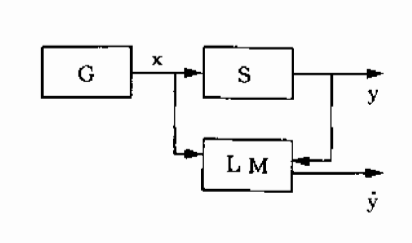
\includegraphics[width=0.4\textwidth]{img/vapniksetting.png}
    \caption{A model of learning from examples. During the learning process, the learning machine observes the pairs $(x, y)$ (the training set). After training, the machine must on any given return a value $j$. The goal is to return a value $y$ that is close to the supervisor's response $y$. We will use this interpretation in the experimental setting. Reused from \cite{Vapnik1999-VAPTNO}}
\end{SCfigure}

We adopt this for our own scheme, which is represented as in Figure~\ref{fig:vapnik_scheme}. This scheme is also used in developing and considering all possible further algorithms and experiments. 
\begin{figure}[htb]
  \centering
  \includegraphics[width=0.7\textwidth]{Diagramatic_Modelling_View.png}
  \caption{\textbf{Diagrammatic view for the ambiance space of the modelling scenario setting.} Under classical learning theory and consideration, such scheme is used for almost every aspect possible of the learner's action. $c\in\mathcal{C}, h\in \mathcal{H}$ described by the tuple $(\mathbf{w},\mathbf{s})$ of main (weight) parameters and special parameters (for example, bias), $\mathbf{I}$ as the input space. The 3-tuple $(\omega, k,m)$ is used for controlling the partitioning (for $k=2$ is the train-test split). Others include $P(\mathbf{I},c,h,\mathcal{D}_{c})$ as the theorized action sequence (where the concept is exhibited, or the where the observational space is formed) of supposed distribution $\mathcal{D}_{c}$, the supervisor $\text{Supervisor}(\nabla, \mathcal{A}, \{\Theta_{S}\})$ for the loss class $\nabla$, algorithm $\mathcal{A}$, and $\{\Theta_{S}\}$ of special parameters for the supervisor. Additionally, we also include the supposed randomized state generation, $\mathsf{RAND}_{i}(\theta_{i,j,k})$ of distinct controlling parameters and arbitrary pseudo-random shape.}
  \label{fig:vapnik_scheme}
\end{figure}


\subsection{Observation 1 - Univariate standard function models}

Univariate refers to the singular case for $\mathbf{X}$ with single parameter $x$. This is also where we get the term overfitting and underfitting, however, in reverse direction. First, we determine our course of action by determine the complexity here. 

The complexity is rather both convenient and difficult. We can safely use the structural mass of the parameter-count type. However, we consider also the finite copula, or multiplicative power of each individual parameter. Thereby, we consider the complexity measure $M(\mathcal{F})$ on the function class $\mathcal{F}$ of univariate, finite coefficient as containing both the structural mass and the expressive complexity. For structural mass, we take the form $M_{\alpha}= p+1$ for parameter counts, with the additive one refers to the constant of addition in those function class. For expressive complexity, we have to take into account of several factors. 

The following lists all the elementary function class used in such particular research. 

\begin{table}[htb]
  \centering
  \begin{tabularx}{\textwidth}{L{2cm} L{3cm} Y}
    \toprule
    Function class & Expression & Compound model form\\
    \midrule
    Linear & \(a x + b\) & None \\
    Polynomial & \(\displaystyle \sum_{i=0}^{k} a_{i} x^{i}\) &
        $p(x)q(x)=\sum_{k}\Big(\sum_{i+j=k} a_i b_j\Big)\,x^k$\\
    Exponential & \((a/b)\,\exp(bx+d)+e\) &
    \(\displaystyle \sum_{n} c_n e^{\lambda_n x}\)
    \\
    Trigonometric & \(a\sin(bx+d)+e\) &
    \(\displaystyle \sum_{n=0}^{\infty}\big(A_n\cos(nx)+B_n\sin(nx)\big)\)
    \\
    \bottomrule
  \end{tabularx}
  \caption{\textbf{Elementary function classes and their respective parameter-control / compound forms on unitary $\mathbb{R}$-space}. For linear we do not expand into a compound; polynomials admit coefficient convolution under multiplication,
    exponentials admit sums of exponentials (Proxy / exponential sums), and trigonometric functions admit Fourier-series decompositions. Analytical expression and complexity analysis of exponential and trigonometric class can be reduced to singular network, however their expressive complexity is harder to define. 
  }
\end{table}

For them, the most simple ones are linear and polynomial class, since they are based on fundamental elementary operation, which can then be regarded or graded of certain complexity. The polynomial itself can have special configuration, for example, the Chebyshev-class polynomials. For linear and polynomial form, they are of the already well-formed operational form, which is the parameter-affectant form $a_{i}x^{i}$, which can be easily compared. However, for the other elementary functional form, their \textit{control-added parameters} require a few more considerations. In the exponential form, for example, the `degree of control' is directed as being 
\begin{equation}
  \mathcal{E}(x) : \omega \exp{(bx+d)}+ e = \frac{a}{b} \exp{(bx + d)} + e 
\end{equation}
for elementary values $a,b,c,d,e,\omega \in \mathbb{R}$. As this is the singular form, it can then be expressed in such form easily. However, the effect is rather not well-defined, which is a problem that have to be considered. 

\begin{theorem}[Approximation on univariate form]
  Given a univariate functional space $\mathbf{U}_{\mathbf{w},x}$, there exists at least one $\epsilon > 0$ as noise of the observable on continuous form, such that for a model and concept $h,c\in \mathcal{F}$ of the same function class, then it is guaranteed of a polynomial-time $p(\cdot,\cdot,\cdot,\cdot)$ complexity, $\ell(c,h)\geq 1/\delta$ for $\delta > 0$. 
\end{theorem}
\begin{proof}
  See appendix. This is a special case of the approximation theorem and the PAC-learning construct, assuming same hypothesis and concept class. 
\end{proof}
The result with polynomial and exponential is then presented for a given variational $\epsilon$, within standard gradient descent. To control the stability of changing complexity class, we repeat the experiment with a variable of ensembles. Statistical measure are there to fill in the details. 

\begin{theorem}[Unitary Fourier]
  The class of all Fourier-class models can approximate, in a given range $[a,b]$, of confidence $1/\delta$ and within accuracy $1/\epsilon$ arbitrary unitary function class on $(\mathbb{R},\mathbb{R})$. 
\end{theorem}


The following experiments will justify and investigate all different ordered permutation of models, especially to extract double descent behaviours or not. Interestingly, the system complexity, one of the complexity measure that is of consideration, will be excluded, and is reserved for latter examples. 

\subsubsection{Linear vs all}
We first use linear versus all the other models. A linear model of univariate setting will just be $f_{\mathrm{Lin}}(x)=a_{1}x+a_{2}$ for the set of parameter $a_{1}x+a_{2}$. For the setting, we will not test it against the same class itself, since there exists the guarantee of approximating same class representation for a finite univariate space, for a given $\epsilon > 0$ as noise. 


\subsubsection{Polynomial-vs-all}

\subsubsection{Exponential compound model}

\subsubsection{Fourier-based compound model}

\subsection{Observation 2 - Prescription from \cite{lafon_understanding_2024}}
We reserve the first experimental run for a test and check experiment, so that we can then identify the problem setting more accordingly. The first, and the most simple model that can be taken into account is the model of linear regression with varied setting. The model that is representative of this preliminary observation is from \cite{lafon_understanding_2024}, specifically, linear regression with Gaussian noise. Consider the family class $(\mathcal{H}_p)_{p\in\llbracket1,d\rrbracket}$ of linear functions $h:\R^d\mapsto \R$ where exactly $p$ components are non-zero ($1\leq p\leq d$), we have the following model. 

\begin{definition}
For $p \in \llbracket1,d\rrbracket$, $\mathcal{H}_p$ is the set of functions $h:\R^d\mapsto \R$ of the form:
$$
h(u)=u^Tw,\quad \text{for }u \in \R^d
$$
With $w \in \R^d$ having exactly $p$ non-zero elements. The complexity here itself can be interpreted as the effective random initialization, trimming down data of hidden details instead - this is indicated by the amount of information it observes given $d$ dimension, and $p$-hypothesis dimension. According to the \textit{manifold hypothesis}, there are chances where the actual concept can be interpreted and mimicked by seeing that it lies on a lower-dimension manifold inside its actual expressive dimensional space. 
\end{definition}
Using such model, they consider the setting of minimizing
\begin{equation}
\label{eq:linear_gaussian_erm}
\min_{w\in \R^d} \frac{1}{2}\norm{\bm{X} w - \bm{Y}}^2 \to \min_{w\in \R^p} \frac{1}{2}\norm{\bm{\Xp} w - y}^2
\end{equation}
of the sub-problem on $p$ cardinality. This results in the following theorem that 'mimic' double descent on this linear regression model. 
\begin{theorem}[Double descent on linear regression]
\label{thm:double_descent_lr}
Let $(x, \epsilon)\in \R^d\times\R$ independent random variables with $x \sim \mathcal{N}(0,I)$  and $\epsilon \sim \mathcal{N}(0,\sigma^2)$, and $w \in \R^d$. we assume that the response variable $y$ is defined as $y=x^Tw +\sigma \epsilon$. Let $(p,q) \in \llbracket 1, d\rrbracket^2$ such that $p+q=d$, $\bm{\Xp}$ the randomly selected $p$ columns sub-matrix of X. Defining $\hat w:=\phi_p(\p{\hat w},\q{\hat w})$ with $\p{\hat w}=\bm{\Xp}^+y$ and $\q{\hat w} = 0$.\\
The risk of the predictor associated to $\hat w$ is:
$$
\E[(y-x^T\hat w)^2] = 
\begin{cases}
(\norm{\wq}^2+\sigma^2)(1+\frac{p}{n-p-1}) &\quad\text{if } p\leq  n-2\\
+\infty &\quad\text{if }n-1 \leq p\leq  n+1\\
\norm{\wp}^2(1-\frac{n}{p}) +  (\norm{\wq}^2+\sigma^2)(1+\frac{n}{p-n-1}) &\quad\text{if }p\geq n+2\end{cases}
$$
\end{theorem}
As said, this theorem is designed to mimic the double descent behaviour on the range of linear regression with Gaussian noise. However, the size of the dataset affects if double descent is emitted or not, at least in terms of regression estimation of wide-field testing set. 
%\begin{figure}[htb]
%    \centering
%    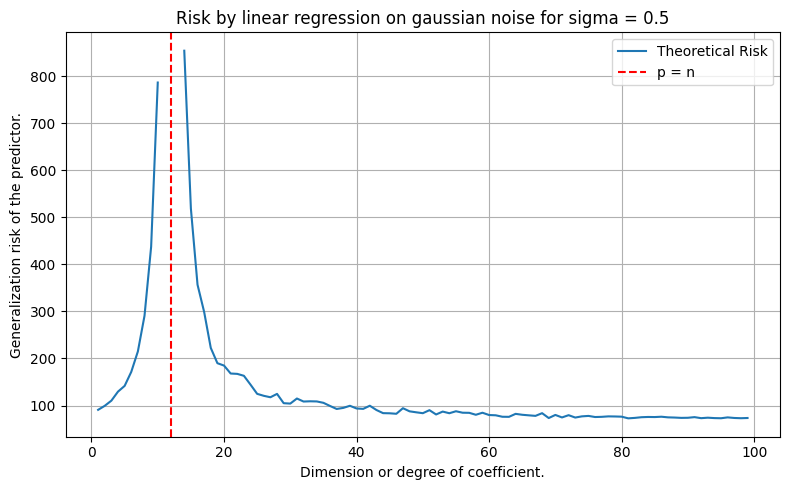
\includegraphics[width=0.5\textwidth]{img/descent_lin_reg_1.png}
%    \caption{Theorem~\ref{thm:double_descent_lr} behaviours on randomized setting. For this model, we have %$d=100$, $\sigma = 0.5$, and variational $n$. This case is for $n=12$.}
%\end{figure}

The first experimental setting is then conducted with fixed $d$, varying $p$ for each varying $n$ samples. Since this is a least square result, preliminary run is conducted using one-shot error-risk measure on least square closed-form approximation. Note that $p\leq d$, hence we are regarding the domain of the term underparameterized and equal parameterization setting. This is illustrated in Fig~\ref{fig:11grid}.

From such data, and setting, we see that for constant noise with expanding dataset, random ordering of such dataset, the analytical solution of best fit turns out to as the risk decomposition, using the above Theorem~\ref{thm:double_descent_lr}, fails to be realized with large $n$ after certain threshold. What is even more interesting, is that as we find out, the above double-descent replicating formula can actually be realized by the parameter-wised error, or 
\begin{equation}
\mathrm{MSE}_{\mathrm{param}}=\left\lvert \hat w - w \right\rvert _{2}^{2}=
\sum_{j=1}^{d}
\left(
  \hat w_{j} - w_{j}
\right)^{2}
\end{equation}
with 
\begin{equation}
\hat w_{j}
=
\begin{cases}
\beta_{p,k}, & j = i_{k} \in S,\\[6pt]
0,           & j \notin S,
\end{cases}
\quad
S = \{\,i_{1},\dots,i_{p}\}.
\end{equation}
and \(S=\{i_1,\dots,i_p\}\) is the set of selected feature indices. The result is represented in Figure~\ref{fig:11grid2}, as per elementary result. While previously mentioned and analysed in Theorem~\ref{thm:double_descent_lr} to be equivalent, in such setting, it is entirely nonexistent. 

If we are to use the standard measure of MSE on model's response, though, the result is rather fairly disappointing, with no trace of double descent in any given way. This is perhaps the more interesting result, as it represents two masks of measure in one setting that might be overlooked. For the formulation
\begin{equation}
\mathrm{MSE}_{\mathrm{pred}}
=
\frac{1}{n}
\left\lVert
  y - X_{p}\,\hat\beta
\right\rVert_{2}^{2}
=
\frac{1}{n}
\sum_{i=1}^{n}
\left(
  y^{(i)} - x_{p}^{(i)\,T}\,\hat\beta
\right)^{2}
\end{equation}
of the standard model, we gain the following result. This also suggest perhaps double descent indeed is coming from some internal fluctuation and aspect that cannot be dissected from another angle, but apparent in some of the model's behaviours, at least intrinsic in the closed-form approximation solution case. 

Thence, the theorem gives us two things - the interpolation point, in this setting, refers to the parameter error for their double descent behaviour. However, on the prediction results' error measure, the interpolation point correlates to the point where the defined generalization risk in such case equals zero. These patterns hold up to certain point. However, the test case is only up to $d=p$. An unexplored test case for $p>d$ indicate the surprising fact according still, to the theorem: the generalization risk takes double descent as a region with disturbance in the middle, but bias-variance appears afterward. This is illustrated in Figure~\ref{fig:contrarian}, where the same theorem is applied but in the domain which is usually called as \textit{overparameterized region}. 
\begin{figure}[htp]
  \centering
  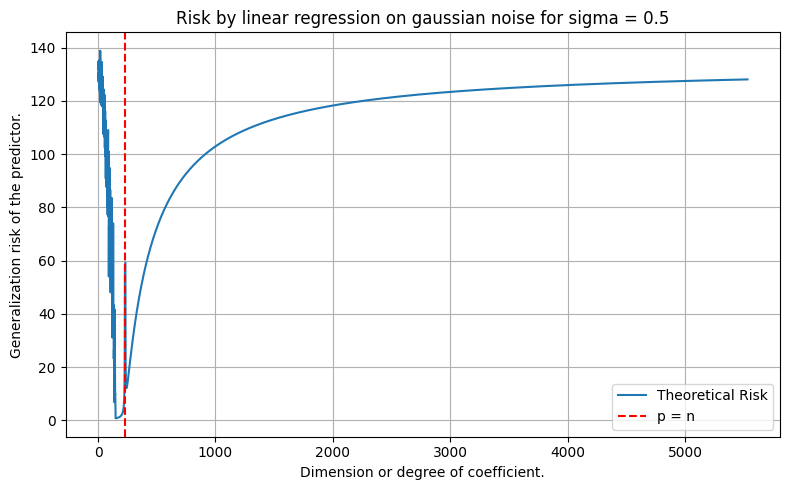
\includegraphics[width=0.6\textwidth]{img/dimensional_descent.png}
  \caption{Similar experiment according to setting and result of Theorem~\ref{eq:linear_gaussian_erm}, where $p$ is in the range [1,5523]. Here, we can see small double descent modelled exactly at the interpolation threshold, while the later region exhibit similar phenomenon as bias-variance tradeoff.}
  \label{fig:contrarian}
\end{figure}

The setting of the theorem and the model itself requires several moving parts in making it to work. 

However, the interpretation of the result is not perfect. Under such setting, then for the concept of the same class, so $d=150$, any concept of $p>d$ would result in the metric taking zero value of the `truncated region' where $d$ is literally flat on the $d+1$ onward space. Hence, the error being added on top of such error measure is the component distance of $p$ to the flat sub $p-d$ space itself - which explains the curve going upward, as more and more risks are configured. Nevertheless, the amount of data provided, at least in terms of this model, does indeed have non-trivial effect on the model itself, and the least square solution of best fit which gives the potential minimal, hence the empirical best. Considering the results, we can see regions where the theorem `breaks' of its bias-variance pattern. Further experiment to verify such claim and reconfiguration is needed. Worryingly, in this particular case, there exists no saddle point that was theorized by bias-variance tradeoff, which must then be explained accordingly. Furthermore, we also notice the troublesome fact that this particular pattern works on \textit{same operational space} models, that is, linear models approximating linear models. This setting is fairly limited, and would not generalize well. However, we also do not know what kind of measure to take in such case. 

\clearpage

\begin{figure}[htb]
  \centering
  \newcommand{\imgwidth}{0.22\textwidth}

  % first row: images 1–4 with n values
  \begin{subfigure}[b]{\imgwidth}
    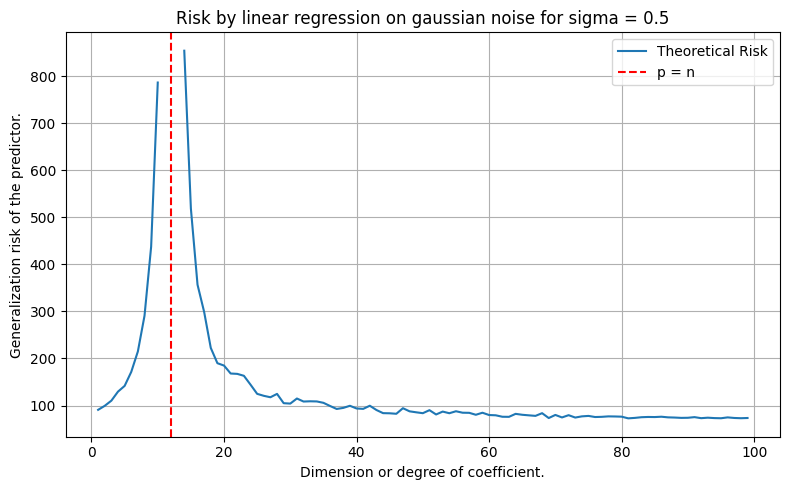
\includegraphics[width=\linewidth]{img/descent_lin_reg_1.png}
    \caption{$n=12$}\label{fig:1a}
  \end{subfigure}%
  \hfill
  \begin{subfigure}[b]{\imgwidth}
    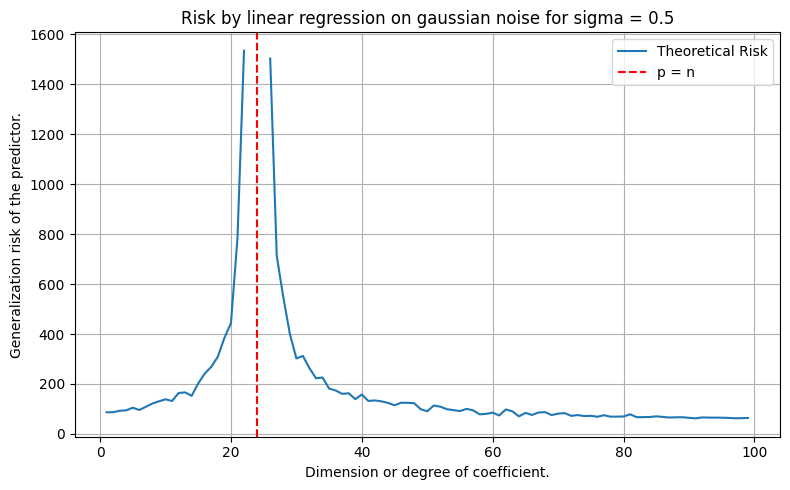
\includegraphics[width=\linewidth]{img/descent_lin_reg_2.png}
    \caption{$n=24$}\label{fig:1b}
  \end{subfigure}%
  \hfill
  \begin{subfigure}[b]{\imgwidth}
    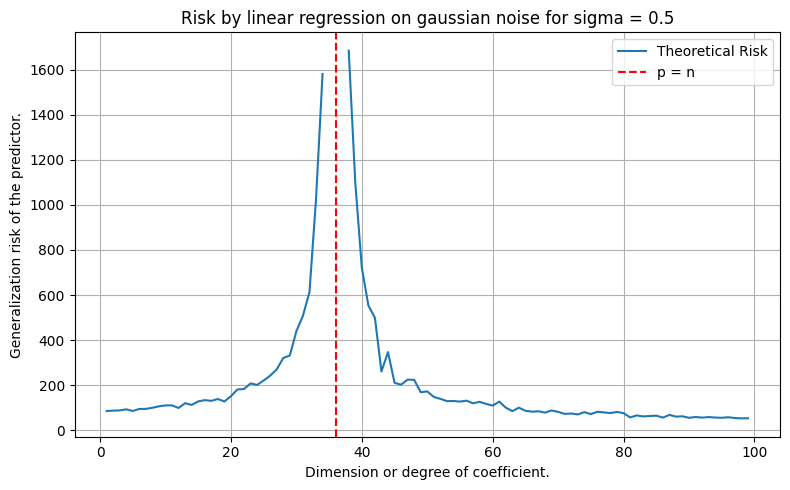
\includegraphics[width=\linewidth]{img/descent_lin_reg_3.png}
    \caption{$n=36$}\label{fig:1c}
  \end{subfigure}%
  \hfill
  \begin{subfigure}[b]{\imgwidth}
    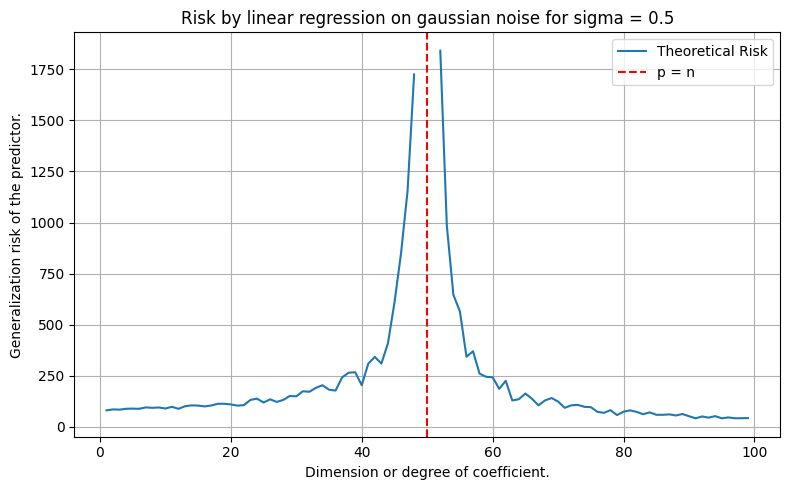
\includegraphics[width=\linewidth]{img/descent_lin_reg_4.png}
    \caption{$n=50$}\label{fig:1d}
  \end{subfigure}

  \medskip

  % second row: images 5–8 with n values
  \begin{subfigure}[b]{\imgwidth}
    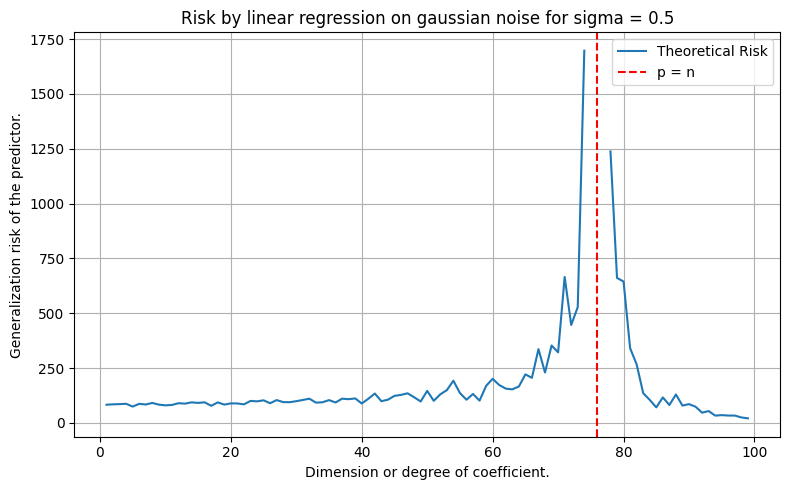
\includegraphics[width=\linewidth]{img/descent_lin_reg_5.png}
    \caption{$n=76$}\label{fig:2a}
  \end{subfigure}%
  \hfill
  \begin{subfigure}[b]{\imgwidth}
    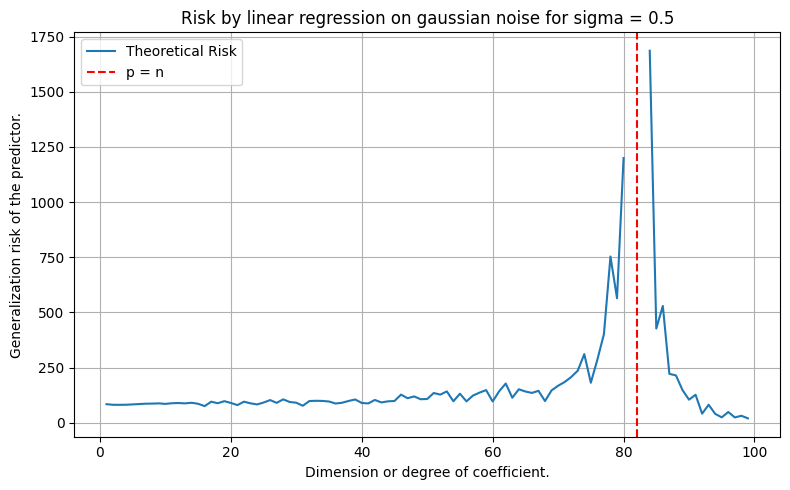
\includegraphics[width=\linewidth]{img/descent_lin_reg_6.png}
    \caption{$n=82$}\label{fig:2b}
  \end{subfigure}%
  \hfill
  \begin{subfigure}[b]{\imgwidth}
    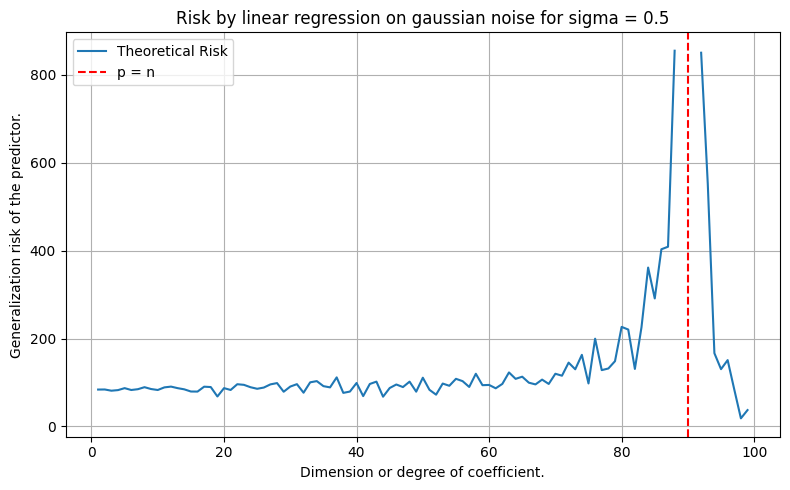
\includegraphics[width=\linewidth]{img/descent_lin_reg_7.png}
    \caption{$n=90$}\label{fig:2c}
  \end{subfigure}%
  \hfill
  \begin{subfigure}[b]{\imgwidth}
    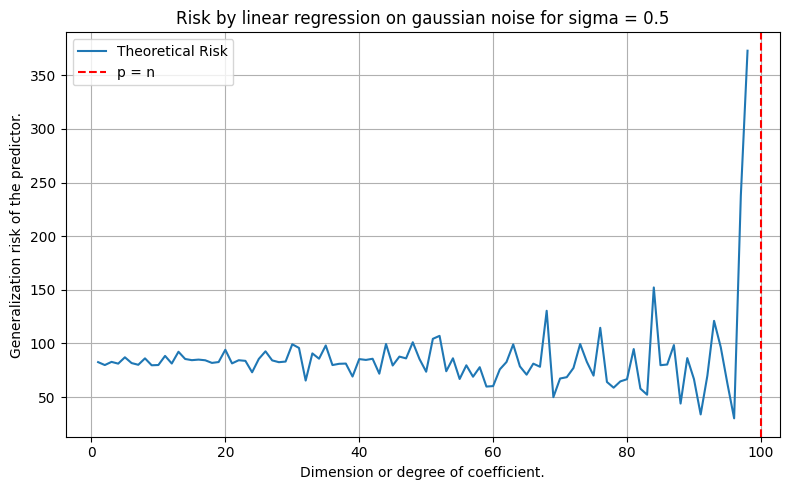
\includegraphics[width=\linewidth]{img/descent_lin_reg_8.png}
    \caption{$n=100$}\label{fig:2d}
  \end{subfigure}

  \medskip

  % third row: images 9–11 with n values
  \begin{subfigure}[b]{\imgwidth}
    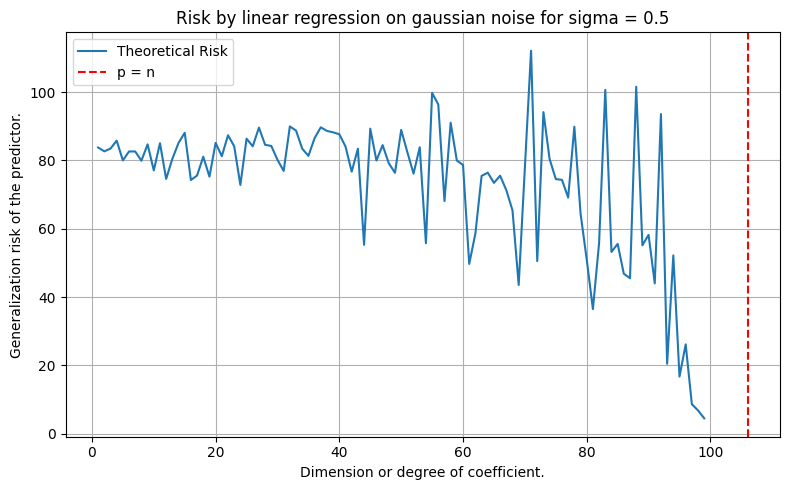
\includegraphics[width=\linewidth]{img/descent_lin_reg_9.png}
    \caption{$n=106$}\label{fig:3a}
  \end{subfigure}%
  \hfill
  \begin{subfigure}[b]{\imgwidth}
    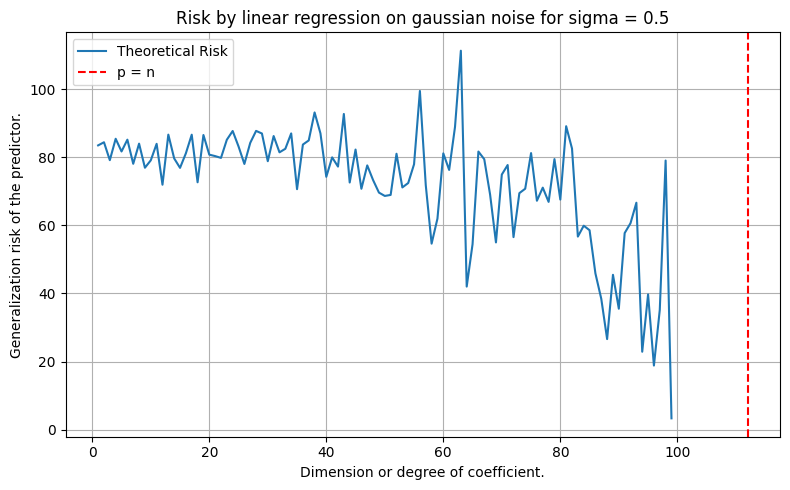
\includegraphics[width=\linewidth]{img/descent_lin_reg_10.png}
    \caption{$n=112$}\label{fig:3b}
  \end{subfigure}%
  \hfill
  \begin{subfigure}[b]{\imgwidth}
    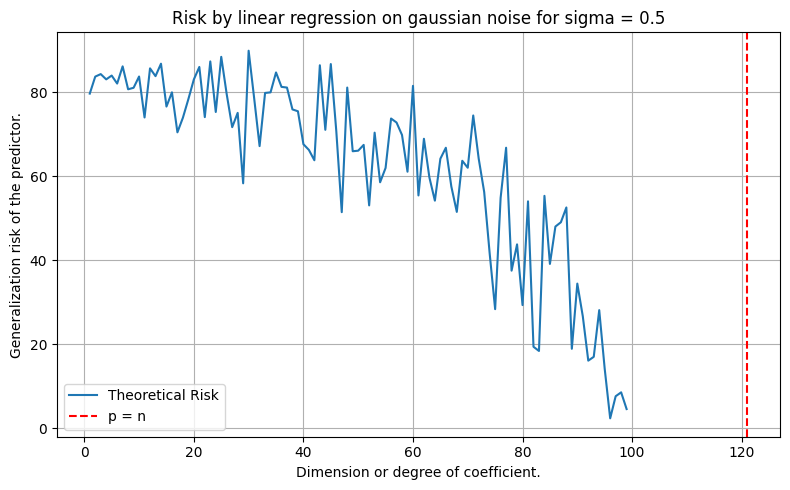
\includegraphics[width=\linewidth]{img/descent_lin_reg_11.png}
    \caption{$n=121$}\label{fig:3c}
  \end{subfigure}%
  \hfill
  \begin{subfigure}[b]{\imgwidth}
    ~
  \end{subfigure}

  \caption{Theorem~\ref{thm:double_descent_lr} behaviours on randomized setting. For this model, we have $d=100$, $\sigma = 0.5$, and variational $n$. Full test cases are for $p=[1,100]$, $n=\{12,24,36,50,76,82,90,100,106,112,121\}$ accordingly. The test function of the concept itself is the same linear model, but with different input only.}
  \label{fig:11grid}
\end{figure}

\begin{figure}[htb]
  \centering
  \newcommand{\imgwidth}{0.22\textwidth}

  % first row: images 1–4 with n values
  \begin{subfigure}[b]{\imgwidth}
    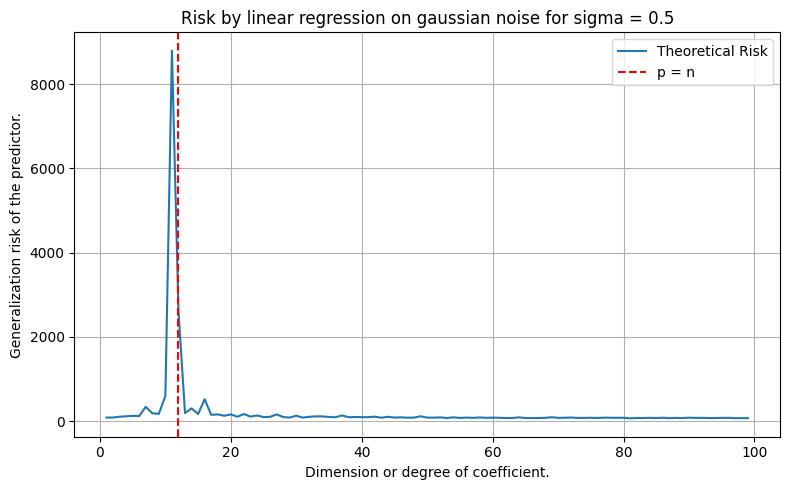
\includegraphics[width=\linewidth]{img/descent_devel1.png}
    \caption{$n=12$}\label{fig:1a2}
  \end{subfigure}%
  \hfill
  \begin{subfigure}[b]{\imgwidth}
    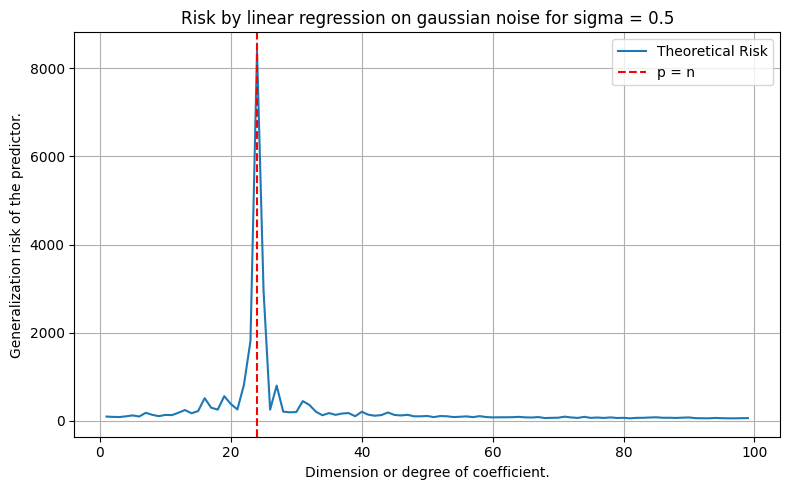
\includegraphics[width=\linewidth]{img/descent_devel2.png}
    \caption{$n=24$}\label{fig:1b2}
  \end{subfigure}%
  \hfill
  \begin{subfigure}[b]{\imgwidth}
    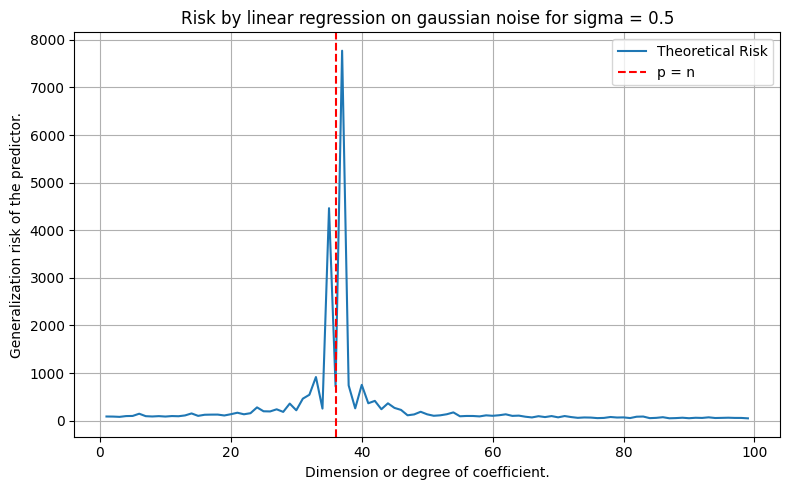
\includegraphics[width=\linewidth]{img/descent_devel3.png}
    \caption{$n=36$}\label{fig:1c2}
  \end{subfigure}%
  \hfill
  \begin{subfigure}[b]{\imgwidth}
    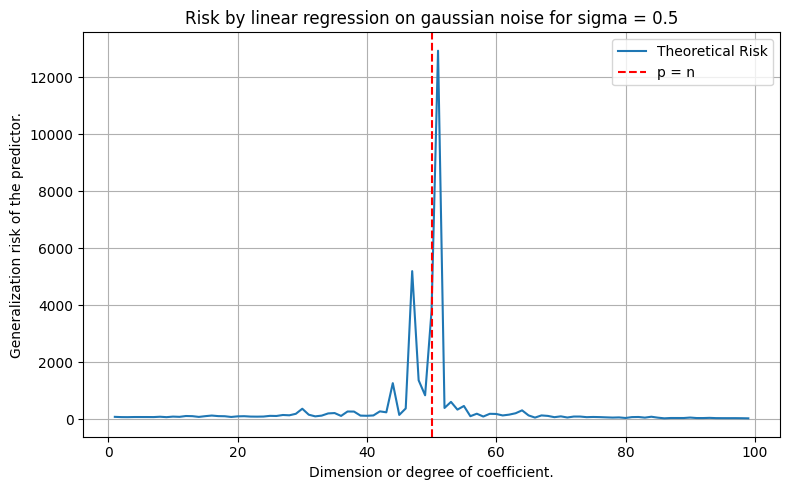
\includegraphics[width=\linewidth]{img/descent_devel4.png}
    \caption{$n=50$}\label{fig:1d2}
  \end{subfigure}

  \medskip

  % second row: images 5–8 with n values
  \begin{subfigure}[b]{\imgwidth}
    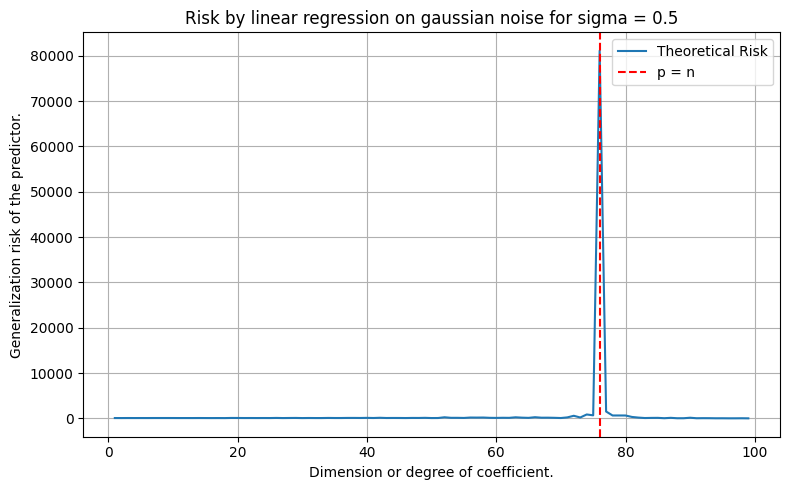
\includegraphics[width=\linewidth]{img/descent_devel5.png}
    \caption{$n=76$}\label{fig:2a2}
  \end{subfigure}%
  \hfill
  \begin{subfigure}[b]{\imgwidth}
    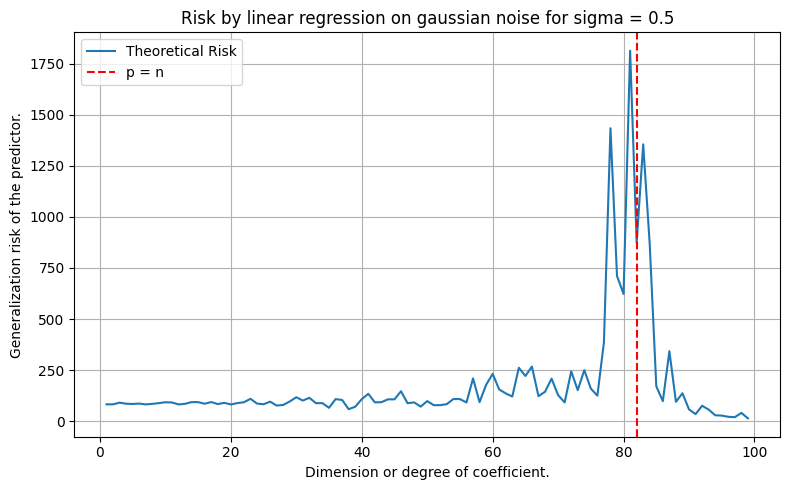
\includegraphics[width=\linewidth]{img/descent_devel6.png}
    \caption{$n=82$}\label{fig:2b2}
  \end{subfigure}%
  \hfill
  \begin{subfigure}[b]{\imgwidth}
    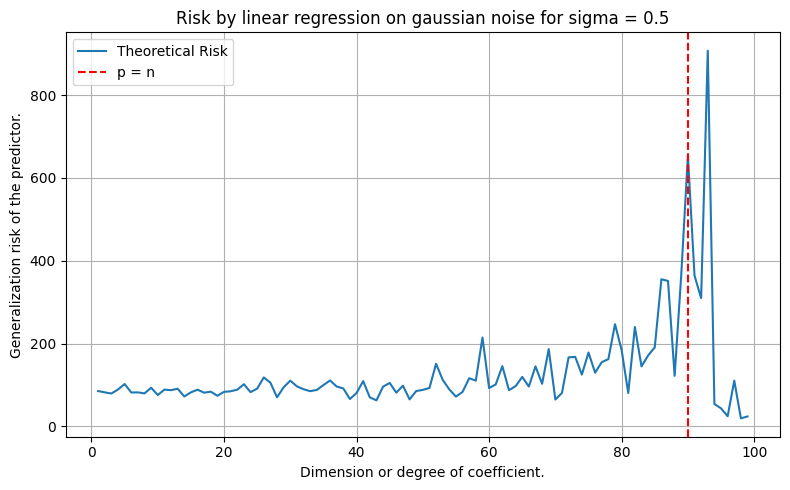
\includegraphics[width=\linewidth]{img/descent_devel7.png}
    \caption{$n=90$}\label{fig:2c2}
  \end{subfigure}%
  \hfill
  \begin{subfigure}[b]{\imgwidth}
    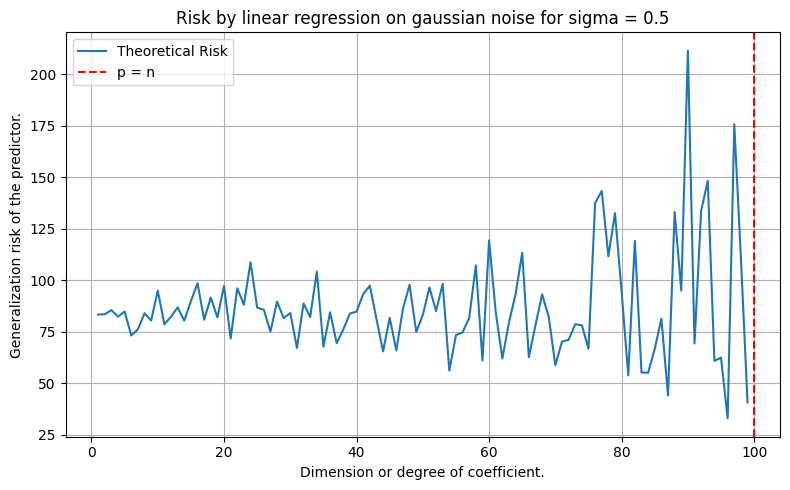
\includegraphics[width=\linewidth]{img/descent_devel8.png}
    \caption{$n=100$}\label{fig:2d2}
  \end{subfigure}

  \medskip

  % third row: images 9–11 with n values
  \begin{subfigure}[b]{\imgwidth}
    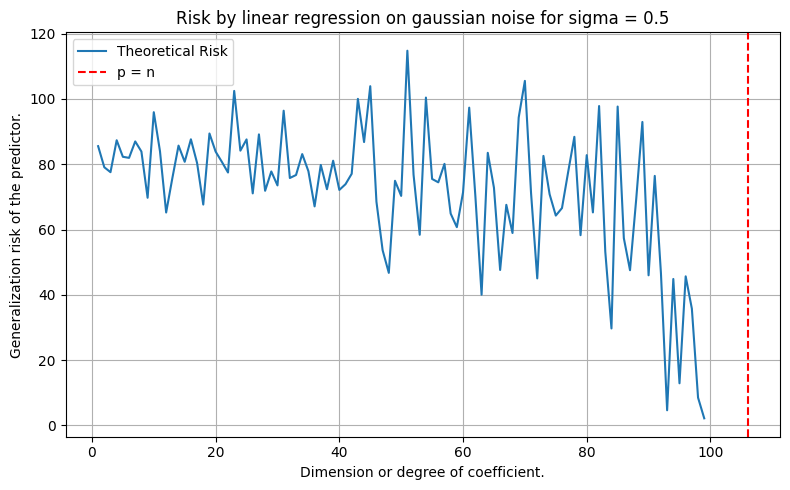
\includegraphics[width=\linewidth]{img/descent_devel9.png}
    \caption{$n=106$}\label{fig:3a2}
  \end{subfigure}%
  \hfill
  \begin{subfigure}[b]{\imgwidth}
    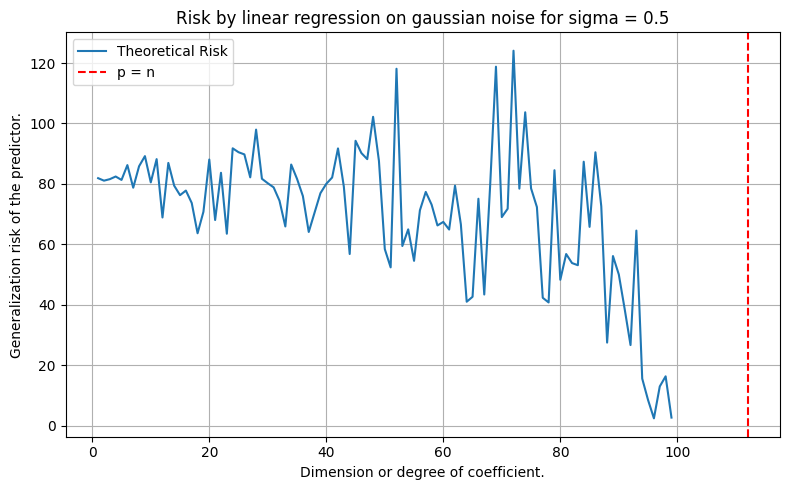
\includegraphics[width=\linewidth]{img/descent_devel10.png}
    \caption{$n=112$}\label{fig:3b2}
  \end{subfigure}%
  \hfill
  \begin{subfigure}[b]{\imgwidth}
    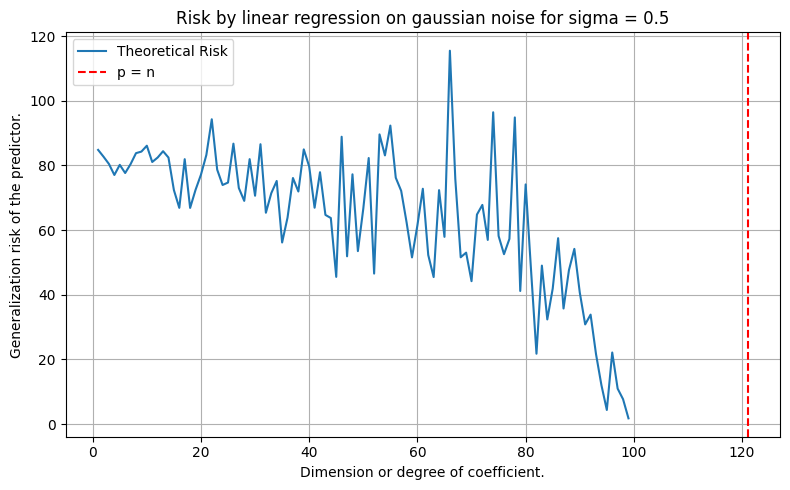
\includegraphics[width=\linewidth]{img/descent_devel11.png}
    \caption{$n=121$}\label{fig:3c2}
  \end{subfigure}%
  \hfill
  \begin{subfigure}[b]{\imgwidth}
    ~
  \end{subfigure}

  \caption{Contrary to Theorem~\ref{thm:double_descent_lr}, this is the behaviours on randomized setting for standard parameter-wised mean square error measure (MSE-on-parameter). For this model, we have $d=100$, $\sigma = 0.5$, and variational $n$. Full test cases are for $p=[1,100]$, $n=\{12,24,36,50,76,82,90,100,106,112,121\}$ accordingly. The test function of the concept itself is the same linear model, but with different input only.}
  \label{fig:11grid2}
\end{figure}

\begin{figure}[htb]
  \centering
  \newcommand{\imgwidth}{0.22\textwidth}

  % first row: images 1–4 with n values
  \begin{subfigure}[b]{\imgwidth}
    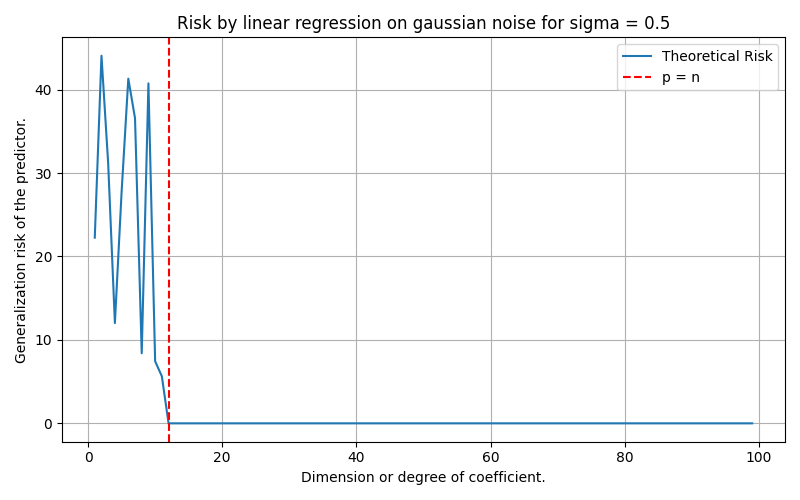
\includegraphics[width=\linewidth]{img/descent_devel_t1.png}
    \caption{$n=12$}\label{fig:1a21}
  \end{subfigure}%
  \hfill
  \begin{subfigure}[b]{\imgwidth}
    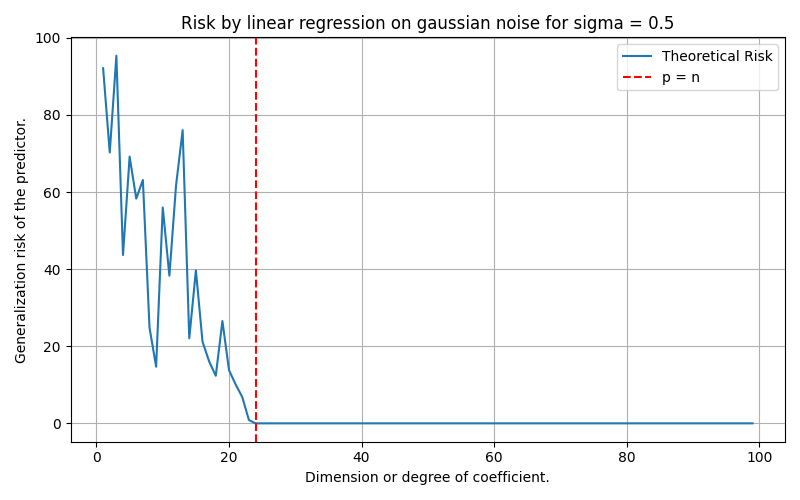
\includegraphics[width=\linewidth]{img/descent_devel_t2.png}
    \caption{$n=24$}\label{fig:1b21}
  \end{subfigure}%
  \hfill
  \begin{subfigure}[b]{\imgwidth}
    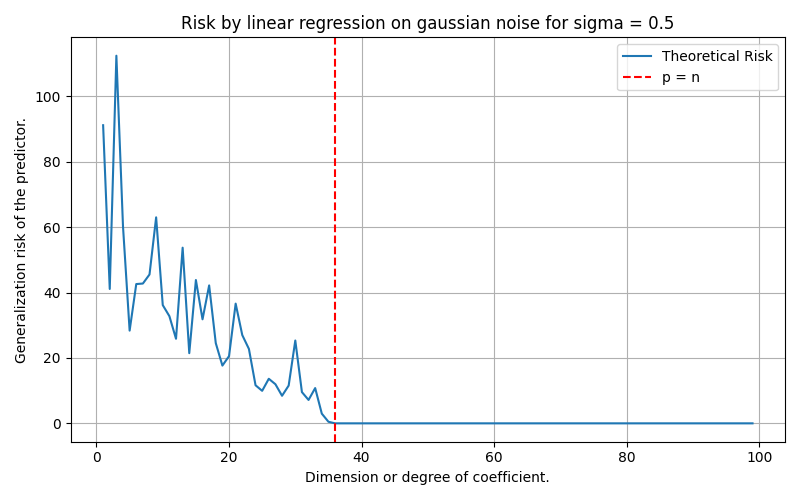
\includegraphics[width=\linewidth]{img/descent_devel_t3.png}
    \caption{$n=36$}\label{fig:1c21}
  \end{subfigure}%
  \hfill
  \begin{subfigure}[b]{\imgwidth}
    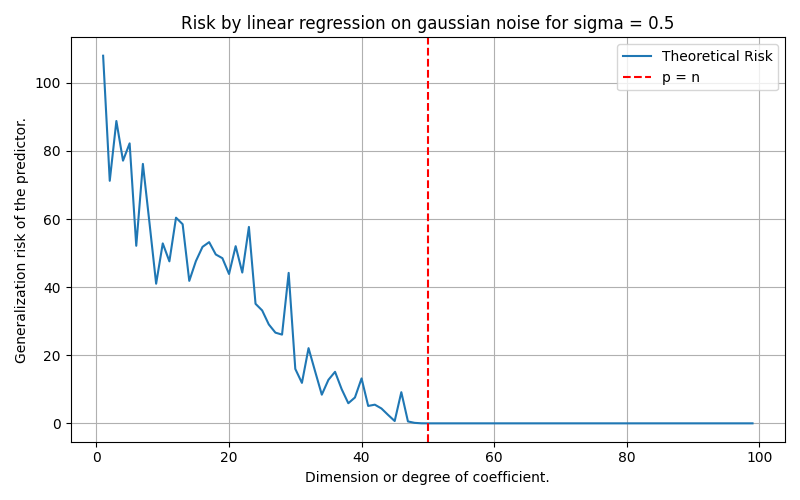
\includegraphics[width=\linewidth]{img/descent_devel_t4.png}
    \caption{$n=50$}\label{fig:1d21}
  \end{subfigure}

  \medskip

  % second row: images 5–8 with n values
  \begin{subfigure}[b]{\imgwidth}
    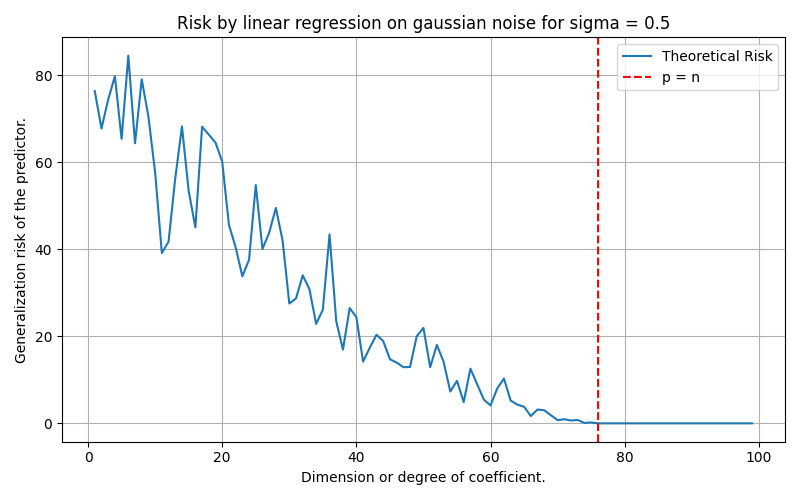
\includegraphics[width=\linewidth]{img/descent_devel_t5.png}
    \caption{$n=76$}\label{fig:2a21}
  \end{subfigure}%
  \hfill
  \begin{subfigure}[b]{\imgwidth}
    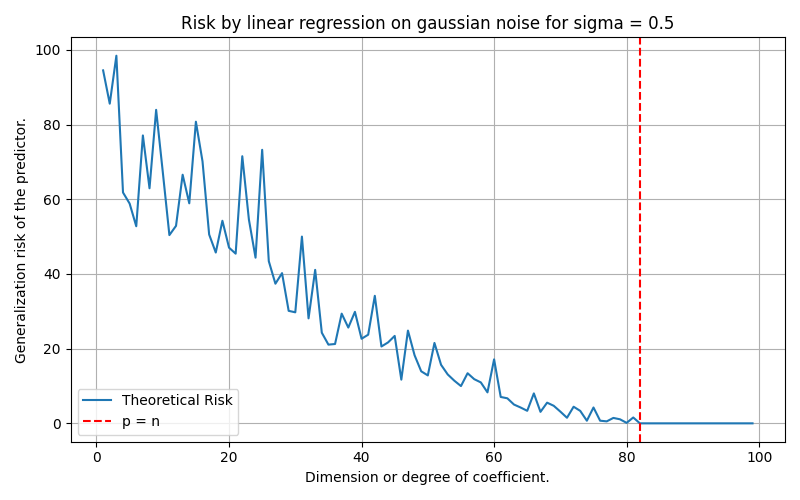
\includegraphics[width=\linewidth]{img/descent_devel_t6.png}
    \caption{$n=82$}\label{fig:2b21}
  \end{subfigure}%
  \hfill
  \begin{subfigure}[b]{\imgwidth}
    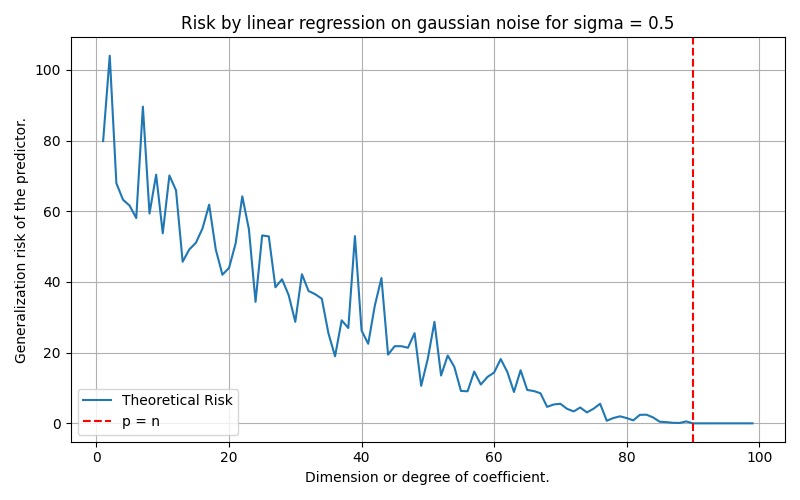
\includegraphics[width=\linewidth]{img/descent_devel_t7.png}
    \caption{$n=90$}\label{fig:2c21}
  \end{subfigure}%
  \hfill
  \begin{subfigure}[b]{\imgwidth}
    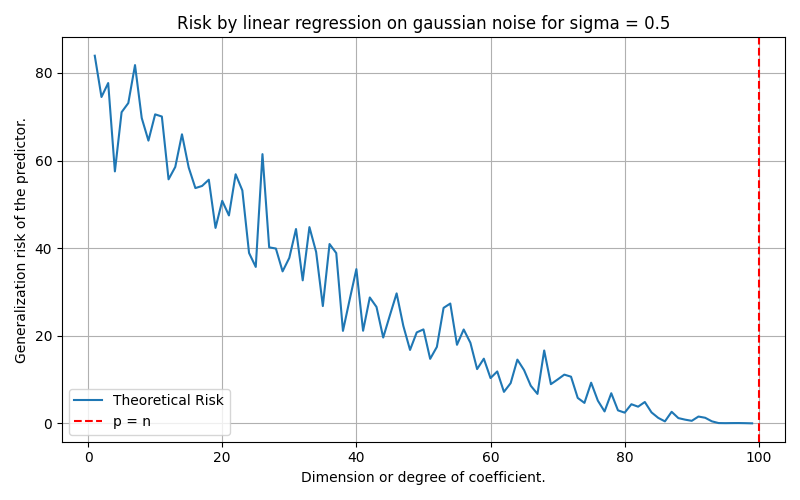
\includegraphics[width=\linewidth]{img/descent_devel_t8.png}
    \caption{$n=100$}\label{fig:2d21}
  \end{subfigure}

  \medskip

  % third row: images 9–11 with n values
  \begin{subfigure}[b]{\imgwidth}
    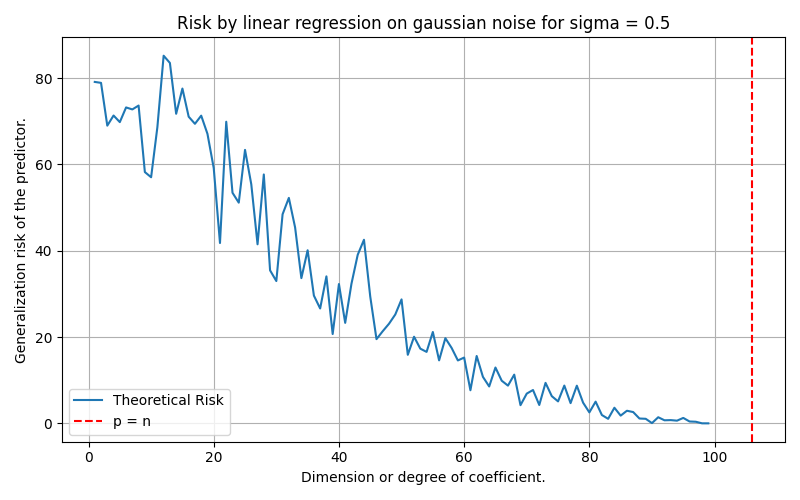
\includegraphics[width=\linewidth]{img/descent_devel_t9.png}
    \caption{$n=106$}\label{fig:3a21}
  \end{subfigure}%
  \hfill
  \begin{subfigure}[b]{\imgwidth}
    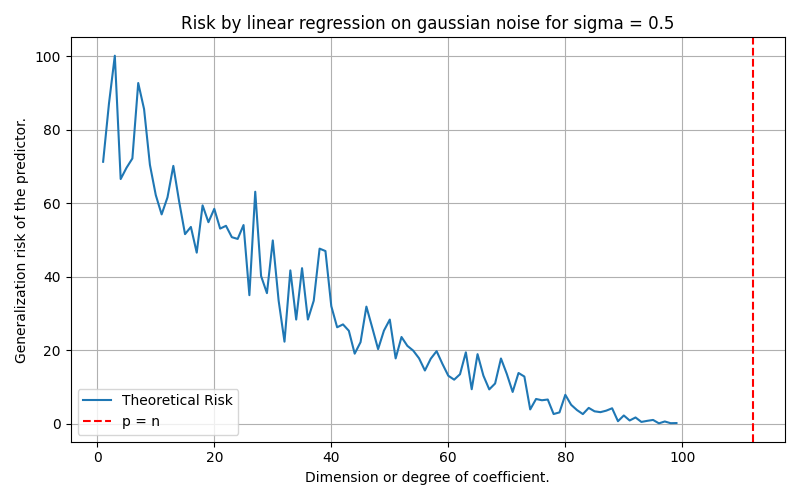
\includegraphics[width=\linewidth]{img/descent_devel_t10.png}
    \caption{$n=112$}\label{fig:3b21}
  \end{subfigure}%
  \hfill
  \begin{subfigure}[b]{\imgwidth}
    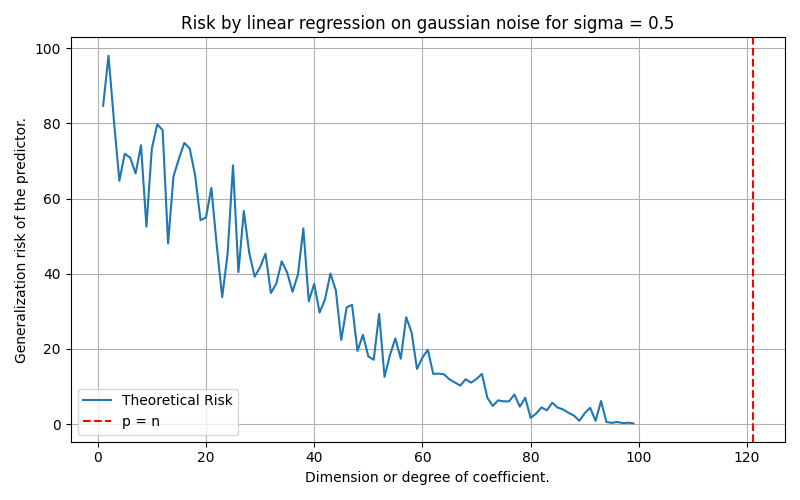
\includegraphics[width=\linewidth]{img/descent_devel_t11.png}
    \caption{$n=121$}\label{fig:3c21}
  \end{subfigure}%
  \hfill
  \begin{subfigure}[b]{\imgwidth}
    ~
  \end{subfigure}

  \caption{Contrary to Theorem~\ref{thm:double_descent_lr} and both figure~\ref{fig:11grid2}, this is the behaviours on randomized setting for standard parameter-wised mean square error measure (MSE-on-prediction). Especially, we do not see double descent pattern in this setting, as it is. For this model, we have $d=100$, $\sigma = 0.5$, and variational $n$. Full test cases are for $p=[1,100]$, $n=\{12,24,36,50,76,82,90,100,106,112,121\}$ accordingly. The test function of the concept itself is the same linear model, but with different input only.}
  \label{fig:11grid21}
\end{figure}

\clearpage 

\subsubsection{Verification}

To verify the theorem itself, we test it with a standard setting without the theorem results. This is reflected in Figure~\ref{fig:risk_all_grid}. The result is somewhat consistent with the theorem and its latter parameter error and prediction error results, however, this time, it correlates exactly as the prediction error instead. Additionally, peculiarity occurs in the non-double descent region, with much less volatility than in the prediction of the theorem. 

We use the Algorithm~\ref{algo:algo_reg_lin_1} for verification, including three modes of error measure, which will then be calculated accordingly. For gradient descent, we refer to another experiment. For such algorithm, we notice that the operational space of the model is $\mathbb{R}^{n}\to \mathbb{R}$. The masking of parameters then is not well-received, since the output space is far more skewed - single dimension resultant with no scaling difference because the model in question is supposed to be linear. Regarding such, it makes sense to realize that the model itself can still attain relatively stable error, because its feature compounds on the scaling parameters.  

To test the stability of the model, we run for a stable section of the permutations done on $p$. The result is outlined in \ref{fig:risk_all_grid}. Interestingly, while the interpolation threshold theorized being $p=n$ does not hold, the pattern of double descent without head descent still fundamentally exists, albeit in a much more constrained region, as can see from $n=12$ to $n=150$. The pattern from then onward follows a reduced trend, without the chaotic behaviours seen. 

\RestyleAlgo{ruled}
\SetKwComment{Comment}{/* }{ */}
\begin{algorithm}
    \caption{Linear regression with Gaussian white noise, full control.}
    \KwData{$n,p,d,\sigma,r$, fixed range $[a,b]$, $u\in [0,1]$}
    \KwResult{Threefold error measure - MSE on parameters $p,d$, MSE on prediction $Y',Y$, and theoretical risks measure by prescription.}
    \Begin
    {
    $\mathrm{Randomizer}(\cdot)\gets\mathrm{PCG64}(n\leq 100)$\Comment*[r]{Randomizing pseudo-random engine}
    $\sigma\gets 0.5$, $d\gets 150$\Comment*[r]{Common presetting for parameters}
    $nl\gets\{12,24,36,50,76,82,90,100,106,112,121,150,231,250,256,280\}$\Comment*[r]{Common full-list $n$ count of datapoints}
    $p\gets 150$\Comment*[r]{Underparameterization to equal}
    $\mathbf{p}\gets \mathrm{range}(1,p)$\; $[a,b]\gets [-100,100]$\;
    $w_{c}\sim \mathrm{PCG64}.\mathrm{Uniform}([1,d],150)$\; $b_{c}\sim \mathrm{PCG64}.\mathrm{Uniform}([1,10])$\;
    $w_{p}\sim \mathrm{PCG64}.\mathrm{Uniform}([1,p],p)$\; $b_{p}\sim \mathrm{PCG64}.\mathrm{Uniform}([1,10])$\;
    $X\sim\mathrm{PCG64}.\mathrm{Uniform}(\mathrm{range}\gets[a,b],\mathrm{size}\gets[n,d])$\Comment*[r]{$n$ samples of $d$ dimensions.}
    $\mathrm{concept}(\cdot,\cdot,\cdot)\gets (d,w_{c},b_{c})$\;
    $Y \gets \mathrm{concept}(X, w_{c},b_{c})$\;
    $\sigma_{\mathrm{scaled}} \gets \sigma \cdot \mathbb{E}\left[\lvert Y\rvert\right]$\;
    $Y \gets Y + \mathrm{PCG64}.…\mathrm{Normal}\left(\mu\gets 0,\;\sigma\gets \sigma_{\mathrm{scaled}},\;\mathrm{size}\gets\lvert Y\rvert\right)$ \Comment*[r]{Noisy featuring}

    \For{$n\in nl$}{
        $w_{p}^{*}\gets\mathrm{PCG64}.\mathrm{Permutation}(d,p)$\;
        \For{$i\gets 1$ \KwTo $\lvert w_{p}\rvert$}{
            \If{$i\neq w^{*}_{p}$}{
                $w_{p}[i]\gets 0$, fixed zero point. 
            }
        }
        $\mathrm{model}(\cdot,\cdot,\cdot)\gets (d,w_{p},b_{p})$\;
        $Y\gets \mathrm{model}(X,w_{p},b_{p})$\;
        $\mathrm{approx}\gets \mathrm{LeastSquare}(\mathrm{model},Y',X,Y)$, fixed $w_{p}$.
    }
    $\mathrm{MSE}_{\mathrm{param}}(\cdot,\cdot,\cdot)\gets \mathrm{MSE}(Y,\{\mathrm{approx}\},\mathrm{model})$\;
    $\mathrm{MSE}_{\mathrm{pred}}(\cdot,\cdot)=\mathrm{MSE}(Y,Y')$
    $\hat{R}_{\mathrm{Thm}}=\mathrm{TR}(w_{c},\sigma,p,d,n)$\;
    }
    \Return{$\mathrm{MSE}_{\mathrm{param}}$, $\mathrm{MSE}_{\mathrm{pred}}$,$\hat{R}_{\mathrm{Thm}}$}
    \label{algo:algo_reg_lin_1}
\end{algorithm}


\begin{figure}[htb]
  \centering
  \newcommand{\imgwidth}{0.22\textwidth}

  % First row
  \begin{subfigure}[b]{\imgwidth}
    \includegraphics[width=\linewidth]{img2/risk_curve_n12.png}
    \caption{$n=12$}\label{fig:2a}
  \end{subfigure}%
  \hfill
  \begin{subfigure}[b]{\imgwidth}
    \includegraphics[width=\linewidth]{img2/risk_curve_n24.png}
    \caption{$n=24$}\label{fig:2b}
  \end{subfigure}%
  \hfill
  \begin{subfigure}[b]{\imgwidth}
    \includegraphics[width=\linewidth]{img2/risk_curve_n36.png}
    \caption{$n=36$}\label{fig:2c}
  \end{subfigure}%
  \hfill
  \begin{subfigure}[b]{\imgwidth}
    \includegraphics[width=\linewidth]{img2/risk_curve_n50.png}
    \caption{$n=50$}\label{fig:2d}
  \end{subfigure}

  \medskip

  % Second row
  \begin{subfigure}[b]{\imgwidth}
    \includegraphics[width=\linewidth]{img2/risk_curve_n76.png}
    \caption{$n=76$}\label{fig:2e}
  \end{subfigure}%
  \hfill
  \begin{subfigure}[b]{\imgwidth}
    \includegraphics[width=\linewidth]{img2/risk_curve_n82.png}
    \caption{$n=82$}\label{fig:2f}
  \end{subfigure}%
  \hfill
  \begin{subfigure}[b]{\imgwidth}
    \includegraphics[width=\linewidth]{img2/risk_curve_n90.png}
    \caption{$n=90$}\label{fig:2g}
  \end{subfigure}%
  \hfill
  \begin{subfigure}[b]{\imgwidth}
    \includegraphics[width=\linewidth]{img2/risk_curve_n100.png}
    \caption{$n=100$}\label{fig:2h}
  \end{subfigure}

  \medskip

  % Third row
  \begin{subfigure}[b]{\imgwidth}
    \includegraphics[width=\linewidth]{img2/risk_curve_n106.png}
    \caption{$n=106$}\label{fig:2i}
  \end{subfigure}%
  \hfill
  \begin{subfigure}[b]{\imgwidth}
    \includegraphics[width=\linewidth]{img2/risk_curve_n112.png}
    \caption{$n=112$}\label{fig:2j}
  \end{subfigure}%
  \hfill
  \begin{subfigure}[b]{\imgwidth}
    \includegraphics[width=\linewidth]{img2/risk_curve_n121.png}
    \caption{$n=121$}\label{fig:2k}
  \end{subfigure}%
  \hfill
  \begin{subfigure}[b]{\imgwidth}
    \includegraphics[width=\linewidth]{img2/risk_curve_n150.png}
    \caption{$n=150$}\label{fig:2l}
  \end{subfigure}

  \medskip

  % Fourth row
  \begin{subfigure}[b]{\imgwidth}
    \includegraphics[width=\linewidth]{img2/risk_curve_n231.png}
    \caption{$n=231$}\label{fig:2m}
  \end{subfigure}%
  \hfill
  \begin{subfigure}[b]{\imgwidth}
    \includegraphics[width=\linewidth]{img2/risk_curve_n250.png}
    \caption{$n=250$}\label{fig:2n}
  \end{subfigure}%
  \hfill
  \begin{subfigure}[b]{\imgwidth}
    \includegraphics[width=\linewidth]{img2/risk_curve_n256.png}
    \caption{$n=256$}\label{fig:2o}
  \end{subfigure}%
  \hfill
  \begin{subfigure}[b]{\imgwidth}
    \includegraphics[width=\linewidth]{img2/risk_curve_n280.png}
    \caption{$n=280$}\label{fig:2p}
  \end{subfigure}

  \caption{Risk curves for varying sample size $n$ (dimension $d=100$, noise $\sigma=0.5$). Double descent is determined in similar sequence, even though the interpolation theoretical $p=n$ is actually shifted over to the right from the actual interpolation observables, in parameterization. Afterward, correlation fails, and the theoretical $p$ is ineffective, similar to previous theorem-based test run. Sample set size range is $n\in\{12,24,36,50,76,82,90,100,106,112,121,150,231,250,256,280\}$. One additional remark is that the error landscape is relatively thin in either side, making it abnormal in comparison to actual bias-variance curvature.}
  \label{fig:risk_all_grid}
\end{figure}

\subsubsection{Remark}

Experiments conducted using Theorem~\ref{thm:double_descent_lr} and variations of it suggests inconsistent results. The supposed interpolation threshold has different interpretation and indication in different scenario, including both parameter-wise error and prediction-only error measure. Furthermore, verification also shows inconsistency with the interpolation threshold, albeit given the fact that the margin of error from the highest peak to the interpolation point is consistent up to certain $n$. Breakdown of the result from theorem, as well as double descent behaviour starts with high $n$ counts, as well as interesting outlook of bias-variance reappearance for $p\sim 5000$, far more than what is tested in normal testing cases. Such result suggests further experiments to validate the observations, as well as statistical analysis of the entire system. 

Additionally, 

\clearpage

\subsection{Observation 3 - Polynomial regression}

For a polynomial model, the complexity measure is harder to grasp. If we treat it the same as the case for linear regression with white Gaussian noise above, we would run into the problem of flattening effect - polynomial explosion of contributing factors between $n$th and the $i$th factor, for $i<n$ is very prevalent. Thereby, we might define the complexity the other way. 

Most of the examples often seen with bias-variance tradeoff is with the famous example of polynomial regression. Indeed, in the range of interpretable, observable model results, polynomial regression with expressive capacity increased is one of the more famous problem setting, which also lies in the regression learning task. \cite{goodfellow2016deep} also used polynomial regression in his book to illustrate the problem of bias-variance tradeoff, and several textbooks, such as ISLR \cite{gareth_james_introduction_2013}. 

Informally, polynomial regression considers the set of all hypotheses $h$ of the polynomial hypothesis class $\mathcal{H}_{p}$. In the single, univariate case of the hypothesis representation, the polynomial $p_{n}(x)\in \mathcal{H}_{p}$ is expressed by: 

\begin{equation*}
    p_{n}(x)=\sum^{n}_{i=0}c_{i}x^{i}
\end{equation*}
where $c_{i}$ is the associated constant for each term. The bias term here is controllable, and is part of the polynomial as the mathematical formulation holds. As always, since it is a model, $x$ argument cannot be controlled. The only degree of freedoms provided is the set $\{ c_{i} \}$ of all constants. Hence, we can conceptualize this as always, as a bunch of unit processing embedded each unit, with a scaling factor by $i$, and control them by the weight. The form $p_{n}(x)$ in a polynomial regressor will often be $M[p(n,x)]=\mathbf{W}f(\mathbf{x})^{\top}$where $f:\mathbb{R}^{n+1}\to \mathbb{R}^{n+1}$ function which scales by applying power per argument. As standard, we will use the typical stochastic gradient descent \footnote{As for why it is not pure vanilla gradient descent, we notice that for a gradient descent algorithm in an informal setting, it is wise to notice that for any given configuration dataset space, the path itself is deterministic based on all the description of the dynamical system (hyperparameters like learning rates, the algorithm itself, the hypothesis's parameters and representation, and the data assumptions - for example, without white noise or not). Removing determinism can be done using stochastic gradient descent, even though for now a formal treatment of this 'stripping off deterministic behaviour' is not fully formulated. }, though it is important to note why we have to use it. 

Using the Ruffini-Horner's scheme, we can analyse the polynomial in the form of nested form: 
\begin{equation}
P(x) = \sum^{n}_{i=0}c_{i}x^{i} = a_0 + x\bigl(a_1 + x\bigl(a_2 + \cdots + x\,(a_{n-1} + x\,a_n)\bigr)\bigr)
\end{equation}
or recursively, as the set of recursive relations
\begin{equation}
  \begin{cases}
b_n               &= a_n,\\
b_k               &= a_k + x\,b_{k+1}, \quad k = n-1, n-2, \dots, 0,\\
P(x)              &= b_0.
\end{cases}
\end{equation}
Experimentally, we would likely have to present certain interpretation and configuration to the setting, depends on particular subject of interest. So far, this is most presentable using diagram.

\begin{setting}[Polynomial testing]
    We formulate the polynomial testing scenario as followed. Let the hypothesis of the class of all univariate, multi-dimension input $\mathbf{x}\in\mathbb{R}^{d}$, for $h\in \mathcal{H}_{p(n)}$ of all univariate polynomial of degree $n$. Let the concept $c\in \mathcal{C}_{p(m)}$ be also the class of all univariate polynomial of degree $m$. Assume that $h$ does not know anything about the true shape of $c$, except for the fact that it is chosen for this purpose by external factor (testing scenario and designer). Consider the observational space $\mathbb{O}$ of $h$. Then, it will be controlled of $\mathbb{O}=(\mathbb{U},\mathbb{I})$ where $\mathbb{U}$ is the \textbf{input space}, and $\mathbb{I}$ is the inferred space. For $\mathbf{x}\in \mathbb{U}\subset \mathbb{R}^{d}$ is governed by the sampling process within distribution of $\mathcal{D}$, and for the inferred space to be of the form $c_{i}+\lambda\mathcal{N}(\cdot)$ of any given noisy feature of certain formulation of scaling $\lambda$. If $\mathcal{N}(\sigma, \mu)$ then we say the inferred space is fully realized as the white noise inferred space. The goal is then to measure, for supposed $\mathsf{ERM}(h,c)$ of the learning process, and $\mathsf{SRM}(h,c)$ for learning process with minimal generalization capacity on $R(h)$, observe and examine the behaviour of the polynomial setting around the interpolation point and within limits of exhibiting double descent. 
\end{setting}
The complexity measure on the surface (operational) would be the degree $n,m$ of the hypothesis and the concept (respectively with the setting), the degree of noise (hence variations) and type of noise, the input space width for $\mathbf{x}\in \mathbb{R}^{d}$ - for it if being high dimensional means more flexibility - which is inherent of the data, and other hyperparameters typical of controlling standard behaviours for the supervisor's learning procedure. In the experimental session, we would also want to somewhat compare the noise fitting solution, to the best interpolation solutions set, to be able to see the interpolating shape after noise. This will determine $d(c,c')$.

\clearpage

\subsection{Observation 5 - Support Vector Machine}

Support vector machine, first formally originated from \cite{Vapnik1999-VAPTNO}, is a model inherently, specifically defined for pattern recognition task, and binary classification via an \textit{optimal separating hyperplane}. There are two variants for SVM, namely, for linear and nonlinear hyperplane. 

The SV machine implements the following two precursor ideas: It maps the input vectors $x$, supposed of the setting, into a high-dimensional feature space $Z$ through some nonlinear mapping, chosen a priori. In this space, an optimal separating hyperplane is constructed. By statistical learning theory, Vapnik restricted the function class (as for infinite hypothesis it is impossible to learn) to the class of hyperplanes by 
\begin{equation}
    \langle \mathbf{w}\cdot \mathbf{x} \rangle + b = 0 ; \quad \mathbf{w}\in \mathbb{R}^{n} , b\in \mathbb{R}
\end{equation}
which $\mathbf{w}$ is the controlling weight, $\mathbf{x}$ is the input space to the space of all binary $\{-1,+1\}$ category. Hence, this basically divide the input space into two: one part containing vectors of the class $-1$ and the others being $+1$. If there exists such a thing, then it is said to be \textit{linearly separable}. To find the class of a particular vector $\mathbf{x}$, we use the following decision function 
\begin{equation}
    f(\mathbf{x}) = \mathrm{sgn}[\langle \mathbf{w}\cdot \mathbf{x}\rangle+ b]
\end{equation}
This is called the \textbf{hyperplane classifier} class. As can be understood simply from such, there exists many hyperplanes that can correctly classifies the classes. It has been then shown that the hyperplane that guarantees the best generalization problem performances is the one with the maximal margin of separation between two classes \cite{Cristianini2000AnIT}. The above form of finding final classification can then be presented in dual form, which then depends only on dot products between vectors, as 
\begin{equation}
    f(\mathbf{x}) = \mathrm{sgn}\left(\sum^{\ell}_{i=1} y_{i}\alpha_{i} \langle \mathbf{x}\cdot \mathbf{x}_{i} \rangle+ b\right)
\end{equation} where $\alpha_{i}\in \mathbb{R}$ is a real-valued variable that can be viewed as a \textit{measure} of how much informational value $\mathbf{x}_{i}$ has (for $x_{i}$ the support vectors we get from training)\footnote{The \textit{support vector} of a particular hyperplane $\mathbf{y}$ is the collections of all points that lies closest to the hyperplane, which is specified as condition for maximization on both side of maximal margin vector machine.}

The second idea is of the \textit{kernel method}. This particular method, useful and well-known of the time SVM was created, gain a more prominent position among other techniques, including neural network. Specifically, this method is characterized by the mapping of the input vectors into a richer (usually high-dimensional) feature space where they satisfy \textit{linear separable} criteria. This prompted the possibility to solve nonlinear problem through such mapping, and indeed yields a nonlinear decision surface in the input space, which is linear in the feature space. A \textbf{kernel} (function) is then a function $k(\mathbf{x},\mathbf{y})$ that given two vectors in input space, return the dot product of their images in feature space such that $k(\mathbf{x},\mathbf{y})=\langle \phi(x), \phi(y) \rangle$ for the nonlinear mapping $\phi$. The general form of SVM is then 
\begin{equation}
    f(\mathbf{x}) = \mathrm{sgn} \left(\sum^{\ell}_{i=1} y_{i}\alpha_{i}k\langle \mathbf{x}\cdot \mathbf{x}_{i} \rangle\right)
\end{equation}
for any particular final categorization. One of the major problem for analysing SVM, is in the properties of it potentially having infinitely many parameters, depends on the size of the dataset. This makes the curve of both bias-variance and double descent not applicable in such regard - infinitely many parameter complexity, yet still finite complexity class. 

From such observation, it would seem imperative that the notion of complexity based solely on the parameter counts of certain model construction is ill-equipped for certain flavours of machine learning model, in this case support vector machine (in the same type is the Gaussian Mixture Model). No double descent has been observed by empirical reports record per the author's knowledge. 

\begin{setting}[Support vector machine]
    We formulate the support vector machine scenario as followed. Let the hypothesis be the class of all $d-1$-dimensional hyperplane opr affine subspace of $d$-dimensional space equipped with kernel, support vectors, and a binary decision rule $\sign{x}\to \{0,1\}$ accordingly. Let the concept $c\in \mathcal{C}$ be the class of all binary categorization that either linearly separable or not. Assume a generalized kernel, $h$ holds no knowledge of $c$ aside from binary separation criteria inherent in its design. Consider the set of observations $\mathbb{O}$ of $h$. Then, it will be controlled of $\mathbb{O}=(\mathbb{U},\mathbb{I})$ where $\mathbb{U}$ is the \textbf{input space} for $k$ points, and $\mathbb{I}\subseteq \{0,1\}^{k}$ is the inferred space of such points. Assume such observations are formed of the distribution $\mathcal{D}^{k}$ on all points. Consider a random $d$-dimensional noise (similar to 1-step random walk) $\mathcal{N}(\cdot)$ or normal distribution $\mathcal{N}(\sigma, \mu)$. The learning process then continues as binary classification for either minimization, and accordingly structural minimization. 
\end{setting}

The complexity in question that would have to be considered and calculated is the support vectors, or rather, the margin point. Though this effectively means that it does not take all data to form the margin, it still means that there then can exist infinite `counting complexity' with respect to the parameter counts. Thereby, we would need another measure of complexity than just as parameters specific to the hypothesis. In fact, the construction of the hypothesis must also consider this aspect itself as a class. 

We tested preliminary SVM with dimension of the feature $p$ in range $[1,80]$, linear kernel, data points increase of the sequence $\{5, 10, 20, 30, 40 , 50, 60, 70 , 80, 100, 120, 140, 150, 160, 170\}$, noise $\sigma = 0.1$, and with distributions almost all being standard normal distribution. Train-test variation is configured with partition scale $0.2$ with random shuffling. Preliminary experiment unfortunately does not give any indication of particularly double descent, and is rather very chaotic. Let us illustrate it. The first case, for $n=20$, normalized, $p=[1,30]$, $\sigma =0.5$, and standard no regularization gives the result in Figure~\ref{fig:test_svm_com_ideal}.

\begin{figure}[htb]
  \centering
  \includegraphics[width=0.5\textwidth]{test_case_ideal_svm.png}
  \caption{\textbf{Experiment on support vector machine on parameterized double descent identification}. The pattern appears marginally on the result graph, with a correct case of interpolation prediction for $p=n$.}
  \label{fig:test_svm_com_ideal}
\end{figure}
However, when we turn our attention to a wider experimental analysis, we gain the following results in Figure~\ref{fig:risk_all_grid_svm}, which is very chaotic. Further experiment is required to validate hypothesis about both, in certain cases, manifold hypothesis's contribution and double descent. 

\begin{figure}[htb]
  \centering
  \newcommand{\imgwidth}{0.22\textwidth}

  % First row
  \begin{subfigure}[b]{\imgwidth}
    \includegraphics[width=\linewidth]{img_qq/risk_curve_n5.png}
    \caption{$n=12$}\label{fig:2a1}
  \end{subfigure}%
  \hfill
  \begin{subfigure}[b]{\imgwidth}
    \includegraphics[width=\linewidth]{img_qq/risk_curve_n10.png}
    \caption{$n=24$}\label{fig:2b1}
  \end{subfigure}%
  \hfill
  \begin{subfigure}[b]{\imgwidth}
    \includegraphics[width=\linewidth]{img_qq/risk_curve_n20.png}
    \caption{$n=36$}\label{fig:2c1}
  \end{subfigure}%
  \hfill
  \begin{subfigure}[b]{\imgwidth}
    \includegraphics[width=\linewidth]{img_qq/risk_curve_n30.png}
    \caption{$n=50$}\label{fig:2d1}
  \end{subfigure}

  \medskip

  % Second row
  \begin{subfigure}[b]{\imgwidth}
    \includegraphics[width=\linewidth]{img_qq/risk_curve_n40.png}
    \caption{$n=76$}\label{fig:2e1}
  \end{subfigure}%
  \hfill
  \begin{subfigure}[b]{\imgwidth}
    \includegraphics[width=\linewidth]{img_qq/risk_curve_n50.png}
    \caption{$n=82$}\label{fig:2f1}
  \end{subfigure}%
  \hfill
  \begin{subfigure}[b]{\imgwidth}
    \includegraphics[width=\linewidth]{img_qq/risk_curve_n60.png}
    \caption{$n=90$}\label{fig:2g1}
  \end{subfigure}%
  \hfill
  \begin{subfigure}[b]{\imgwidth}
    \includegraphics[width=\linewidth]{img_qq/risk_curve_n70.png}
    \caption{$n=100$}\label{fig:2h1}
  \end{subfigure}

  \medskip

  % Third row
  \begin{subfigure}[b]{\imgwidth}
    \includegraphics[width=\linewidth]{img_qq/risk_curve_n80.png}
    \caption{$n=106$}\label{fig:2i}
  \end{subfigure}%
  \hfill
  \begin{subfigure}[b]{\imgwidth}
    \includegraphics[width=\linewidth]{img_qq/risk_curve_n100.png}
    \caption{$n=112$}\label{fig:2j1}
  \end{subfigure}%
  \hfill
  \begin{subfigure}[b]{\imgwidth}
    \includegraphics[width=\linewidth]{img_qq/risk_curve_n120.png}
    \caption{$n=121$}\label{fig:2k1}
  \end{subfigure}%
  \hfill
  \begin{subfigure}[b]{\imgwidth}
    \includegraphics[width=\linewidth]{img_qq/risk_curve_n140.png}
    \caption{$n=150$}\label{fig:2l1}
  \end{subfigure}

  \medskip

  % Fourth row
  \begin{subfigure}[b]{\imgwidth}
    \includegraphics[width=\linewidth]{img_qq/risk_curve_n150.png}
    \caption{$n=231$}\label{fig:2m1}
  \end{subfigure}%
  \hfill
  \begin{subfigure}[b]{\imgwidth}
    \includegraphics[width=\linewidth]{img_qq/risk_curve_n160.png}
    \caption{$n=250$}\label{fig:2n1}
  \end{subfigure}%
  \hfill
  \begin{subfigure}[b]{\imgwidth}
    \includegraphics[width=\linewidth]{img_qq/risk_curve_n170.png}
    \caption{$n=256$}\label{fig:2o1}
  \end{subfigure}%

  \caption{\textbf{Risk plots of support vector machine on incremental $p$ and $n$}. The pattern is not interpretable, albeit we have doubts about the actual result.}
  \label{fig:risk_all_grid_svm}
\end{figure}

\clearpage

\subsection{Neural network}

One more class of elementary and classical experimental setting that would be considered is the class of typical neural network, or in general, $Q$-width $L$-depth neural network of general activation type, without specific engineering or modifications. For completeness, we refer to \cite{zhang2023mathematical} for a more mathematical analysis, and our network will be formulated the same. Generally, we define a $K$-layer fully-connected deep neural network with real-valued output. Let $m^{(0)}=d$ and $m^{(K)}=1$ for $m$ the width of the network, and $d$ the shape of the input vector. We then recursively define: 
\begin{align}
    x_{j}^{(0)} &= x_{j} \quad (j=1,\dots,m^{(0)}),\\ 
    x_{j}^{(k)} &= h\left(\sum^{m^{(k-1)}}_{j'=1} \theta_{j,j'}^{(k)}x_{j'}^{(k-1)}+ b_{j}^{(k)}\right)\quad (j=1,\dots,m^{(k)}), \quad k = 1,2,\dots,K-1\\
    f(x) & = x_{1}^{(K)} = \sum^{m^{(K-1)}}_{j=1} u_{j}x_{j}^{(K-1)}
\end{align}
where the model parameters can be represented by $w=\{[u_{j}, \theta_{j,j'}^{(k)}, b_{j}^{(k)}]: j,j',k\}$ with $m^{(k)}$ being the number of hidden units at layer $k$; $\theta\in \mathbb{R}^{m}$ the weight of the neuron. The setting that we would typically find ourselves in would be function approximation on neural network class. Complexity wise, the neural network depends on three main choices of interest. Either the complexity based on unit counts, that is, the number of layers, and the number of neurons per layer, and the configuration of each neuronal unit - for example, between $\sigma$ sigmoid and ReLU functions. 

For the neural network structure, we would resort to use a general definition instead; however, the task is function approximation. It is defined as the following setting. 
\vspace{2mm}

\begin{setting}
    We formulate the neural network scenario as followed. Let the hypothesis be the class of all $L$-layer fully-connected neural network, for each layer of $i$ standard neuron unit with arbitrary activation functions. Let the operational space be of the field $\mathbb{R}$. The concept $c\in \mathcal{C}[\mathcal{N}_{\ell}]\cup \mathcal{F}$ is to be all neural network class, fully-connected or not, and all function class $\mathcal{F}$. Consider the observational space $\mathbb{O}$ of $h$. Then, it will be controlled of $\mathbb{O}=(\mathbb{U},\mathbb{I})$ where $\mathbb{U}$ is the \textbf{input space}, and $\mathbb{I}$ is the inferred space. For $\mathbf{x}\in \mathbb{U}\subset \mathbb{R}^{d}$ is governed by the sampling process within distribution of $\mathcal{D}$, and for the inferred space to be of the form $c_{i}+\lambda\mathcal{N}(\cdot)$ of any given noisy feature of certain formulation of scaling $\lambda$. If $\mathcal{N}(\sigma, \mu)$ then we say the inferred space is fully realized as the white noise inferred space. The learning process then continues as binary classification for either minimization, and accordingly structural minimization. 
\end{setting}
In a sense, the general setting allows us to configure more than necessary. Furthermore, as will be noted in the neural formalism section, virtually every hypothesis can be somewhat generalized to a neural network. 

\clearpage 

\section{Theoretical analysis}

Since the previous analysis of the learning model, we can then notice a few disadvantages and a few very subtle points that we omitted. It is apparent that the analysis is somewhat entangled, with various situations, interpretations, setting and assumptions together, and with a non-unified structure of models in question. The system in which the model is considered and analyzed is also missing in essence. There are a lot of ambiguities around what is considered and what is not, even with probabilistic nature and the deterministic aspect. Terms like \textbf{latent spaces} and many do not capture the entire dynamic or meaning of the system. It is then we introduce our novel analytical framework, namely the \textbf{Unified Unitary Construct} framework. 
\subsubsection{Motivation}
The predecessors of neural network, for operations and purposes, take in the form of a specific application of function constructs, finite singleton algorithms. For such purposes, a specific classical model $m$ takes the form of a single structure, with complex construction, often offering fixed architecture of its representation. Neural network is an attempt, for its philosophy, to change the aforementioned philosophy of constructing machine model by considering compute unit \cite{mcculloch_logical_1943,Rosenblatt1958ThePA}. 

Recalled the classical learning framework, for $h$. We know and construct the principle of the system by settle on $h:\mathcal{X}\to \mathcal{Y}$, for any arbitrary defined in-out 2-tuple. Hence, the overall construction of a given model can be abstracted into layers of responsive results. 
\clearpage

\section{Physics-inspired perspective 1}
To analyse systems with quenched disorder, such as a neural network trained on a fixed dataset, one must compute the average of the logarithm of the partition function, $\langle\log Z\rangle$, over all possible datasets. This is a mathematically challenging task. The replica method, originating from the statistical mechanics of spin glasses, provides a powerful, albeit non-rigorous, analytical technique using the \textbf{replica trick}:
\begin{equation}
    \mathbb{E}_{\mathcal{D}}[\log Z] = \lim_{n \to 0} \frac{\log \mathbb{E}_{\mathcal{D}}[Z^n]}{n}
\end{equation}
This identity converts the difficult average of a logarithm into an average of an integer power $Z^n$, which is more tractable. The procedure involves introducing $n$ identical, non-interacting copies (replicas) of the system, calculating $\langle Z^n \rangle$, and then analytically continuing the result to the $n \to 0$ limit.

To illustrate, consider a 2-layer committee machine with $K$ hidden units, $N$ inputs, and weights $w_k$ constrained to a hypersphere $||w_k||^2 = N$. The partition function $Z$, also known as the Gardner Volume, measures the volume of weight space satisfying $P$ input-output constraints $(x^\mu, y^\mu)$:
\begin{equation}
    Z = \int \prod_{k=1}^{K} dw_k \delta(N - ||w_k||^2) \prod_{\mu=1}^{P} \Theta(y^\mu s(x^\mu) - \kappa)
\end{equation}
where $s(x^\mu)$ is the network output for input $x^\mu$ and $\Theta$ is the Heaviside step function ensuring a classification margin $\kappa$.

After averaging $Z^n$ over the data distribution, the calculation is managed by introducing \textit{order parameters} that capture the geometric relationships between replicas. By taking the $n \to 0$ limit, we derive a set of coupled saddle-point equations whose solution reveals the typical properties of the solution space, such as the critical storage capacity $\alpha_c = P/N$. This method provides a first-principles approach to understanding how network architecture and data properties jointly determine the geometry of the solution space and the onset of phase transitions in learning. While this canonical example differs from the GNNs that are our primary focus, it serves to illustrate the core methodology: how the replica trick, through the introduction of order parameters, can transform a problem of counting solutions into a tractable analysis of the solution space geometry. We will apply the principles derived here to qualitatively understand the more complex GNN landscape.

\subsection{A Formal Link via PAC-Bayesian Bounds}
We now formalize the connection between the entropy of the solution space and generalization. The Probably Approximately Correct (PAC)-Bayesian framework provides a bound on the true risk $R(Q)$ of a posterior distribution $Q$ over hypotheses (weights):
\begin{equation}
    R(Q) \le \hat{R}(Q) + \sqrt{\frac{KL(Q || P) + \log(m/\delta)}{2m}}
\end{equation}
Here, $P$ is a data-independent prior, $Q$ is the data-dependent posterior, $\hat{R}(Q)$ is the empirical risk on $m$ samples, and $\delta$ is the confidence parameter. The key is the Kullback-Leibler (KL) divergence, $KL(Q || P)$, which measures the information-theoretic "cost" of updating the prior $P$ to the posterior $Q$ after observing the data.

To make this connection rigorous, we introduce the Gibbs posterior, $Q^*_{\lambda}$, which is the optimal choice for $Q$ that minimizes the trade-off $\lambda \hat{R}(Q) + KL(Q || P)$:
\begin{equation}
    Q^*_{\lambda}(h) = \frac{P(h) e^{-\lambda \hat{R}(h)}}{Z(\lambda)}, \quad \text{where} \quad Z(\lambda) = \int P(h') e^{-\lambda \hat{R}(h')} dh'
\end{equation}
This formulation reveals a direct analogy with statistical mechanics:
\begin{itemize}[itemsep=0.5pt,topsep=0pt]
    \item The hypothesis $h$ corresponds to a \textit{state}.
    \item The empirical risk $\hat{R}(h)$ corresponds to the \textit{energy} $E$.
    \item The hyperparameter $\lambda$ corresponds to the \textit{inverse temperature} $\beta = 1/T$.
    \item The normalization constant $Z(\lambda)$ is the \textit{partition function}.
    \item The quantity $F(\lambda) = -(1/\lambda) \log Z(\lambda)$ is the \textit{Helmholtz free energy}.
\end{itemize}
This establishes a rigorous chain of reasoning: a large volume of low-loss solutions (a "flat minimum") implies high entropy $\rightarrow$ which in turn lowers the Helmholtz free energy $\rightarrow$ leading to a smaller KL divergence term in the PAC-Bayesian bound $\rightarrow$ and ultimately certifying better generalization. The partition function, by integrating over all possible solutions weighted by their empirical risk, effectively measures the volume of "good" solutions. Therefore, finding a region in the parameter space with a large volume of low-loss solutions directly translates to a tighter, more robust generalization bound as certified by the PAC-Bayesian framework.

\section{Topological Criticality in Graph Neural Networks}
Statistical physics consideration works well with large-scale system, as their effects are more fluid and better prompted. Thereby, we would want to see the notion of \textit{topological criticality} in terms of graph neural networks, which is the focal point of the last experiment.
\subsection{The Interpolation Peak as a Critical Phenomenon}
We hypothesize that the interpolation peak observed in GNNs is a critical point where generalization error $\epsilon$ diverges according to a scaling law, $\epsilon(k) \sim |k - k_c|^{-\nu}$, where $k$ is model complexity. While analogies to physical systems like the Ising model are instructive, GNNs on heterogeneous graphs exhibit a unique form of criticality.

Unlike a standard second-order phase transition in a mean-field model, where criticality is marked by the divergence of a correlation length, GNNs on large, sparse random graphs (e.g., Barabási-Albert model) can suffer from an expressivity collapse. This is driven by \textit{local weak convergence}: as graph size $N \to \infty$, the local $r$-hop neighbourhood of almost every node converges to a universal random tree structure. Since a $k$-layer GNN's output is solely a function of its $k$-hop neighbourhood, the model's output becomes constant across all nodes, losing all discriminative power.

\begin{table}[h!]
\centering
\small
\caption{Comparison of Criticality Mechanisms}
\begin{tabular}{|p{3cm}|p{4cm}|p{4cm}|}
\hline
\textbf{Property} & \textbf{Ising Model (Mean-Field Analogy)} & \textbf{GNN on a Large Random Graph} \\
\hline
\textbf{Transition Type} & Second-order phase transition. & Expressivity collapse. \\
\hline
\textbf{Governing Concept} & Divergence of correlation length $\xi$. & Local weak convergence of neighbourhoods. \\
\hline
\textbf{Order Parameter} & Magnetization $M$. & Discriminative power of the GNN output. \\
\hline
\textbf{Result} & System develops long-range correlations, described by exponent $\nu=1/2$. & GNN output becomes constant, losing all instance-specific info. \\
\hline
\end{tabular}
\end{table}
The criticality at the GNN interpolation peak is not merely a quantitative divergence but a qualitative shift where the model loses its ability to distinguish between nodes due to fundamental graph topology at scale. We posit that this catastrophic expressivity collapse is the microscopic mechanism responsible for the macroscopic peak in generalization error observed in the double descent curve for GNNs on large, sparse graphs. This reframes the challenge as understanding the architectural and topological conditions that trigger this collapse.

\section{Physics-inspired perspective 2}

Physically speaking, transferring from learning theory to statistical physics, or the like, is difficult. There are the differences between the two fields, and one concept from this place might not exists in the other, even though the explanation might seem relevant. 


\clearpage

\section{Experiments 5 - Graph Neural Networks}
To confirm and observe particular insights on the problem, experimentally, we focus more on the results given by the analysis on a particular type of neural network, the graph neural network (GNN). However, preliminary experiments are also needed, for example, with various complexity and function class, though most of them are algorithm based on ERM, which typically can be called derivation of gradient descent. 

According to major literature, for example, \cite{shi2024homophilymodulatesdoubledescent}, double descent is absent usually in GNN, for example, GCN networks. However, in fact, it is relatively unstable, as for certain papers and researches point out its existence and variation of it being ubiquitous to the network, some reports none of such occurrence in their experiments. Thereby, our first strategy would be to encounter this absence, and the way to force it to exhibit itself, if the phenomenon is perceived non-existent. In experiments by \cite{shi2024homophilymodulatesdoubledescent,buschjager_generalized_2020}, we know that graph network are inherently sensitive to data configuration. The graph MPNN in \cite{GRP_Hamilton}, for example, depends heavily on the configuration of data to present its neighbourhood aggregation for each layer. However, we would like to first claim the dichotomy of bias-variance holds for it to be presented as the first interpolation point.

We would use, and utilizes a hybrid setting between MPNN, GCN and GAN (attention network), to configure out network in itself. However, heterogeneous network - either consists of only MPNN or GCN layers, is somewhat preferred for ease of analysis, and potency of experimental learning control. Because double descent lies between the concept of test error and training error, either supervised or semi-supervised would be used. According to \cite{shi2024homophilymodulatesdoubledescent}, semi-supervised setting gives better flexibility and overall 'range' of operation. Other than GNN, certain more abstract, 'vanilla' neural network formalism as specified in the above section treatment will also be conducted, in a supplementary manner. 

\subsection{Methodology}

Because of the irregularity in the statement that GNN does not exhibit any phenomena that is related to double descent \cite{shi2024homophilymodulatesdoubledescent}, we would be investigating this phenomenon the most. This particularly means that a lot of our focus will be to analyse the GNN network by itself. 

\subsubsection{Quick introduction to graph theory}

A \textbf{graph} $G$ is a 2-tuple $(V,E)$ where $V$ is the set of \textbf{vertices}(or nodes) and $E$ is the set of \textbf{edges}. The set $ne[n]$ stands for the neighbour of vertex $n$, while $co[n]$ is the set of edges that have $n$ as vertex. Edge is often denoted by $(u,v)$ for vertices $u$ and $v$. We said that $(u,v)$ \textbf{joins} $u$ and $v$, and it can be directed or undirected. A graph is called a \textit{directed graph} if all edges are direct or \textit{undirected graph} if all edges are \textit{undirected}. The \textbf{degree} of vertices $v$, denoted by $d(v)$, is $t$ number of edges connected with $v$.
The graph data can be loosely (not specifically in cases) as followed. Let $\mathcal{G}=(\mathcal{V},\mathcal{E},\mathcal{W})$ be a graph, where $\mathcal{V}=\{1,\dots,n\}$ is the set of nodes, $\mathcal{E}=\{1,\dots,M\}\subseteq \mathcal{N}\times \mathcal{N}$ is the set of edges, and $\mathcal{W}: \mathcal{E}\to \mathbb{R}$ is the edge's weight function. There is also the optional weight $\mathcal{W}': \mathcal{V}\to \mathbb{R}$ for each vertex. In this case, it is for certain problem like TVP, where all cities have certain properties for the path. We say that a data sample $\mathbf{x}$ is a graph data, if its entries are related through the graph $\mathcal{G}$. 

\begin{figure}[htb]
  \centering
  \includegraphics[width=0.6\textwidth]{graph_tech.png}
  \caption{
    \textbf{Illustration of an ordering for a specific graph configuration.} We emphasize the perspective to the higher neighbouring degree node in the graph, namely $V_{1}$, and their relative links and connections of the graph itself. A 2-walk (in red) can be seen, which aggregates more to create the 2-neighbourhood of maximally two walks away. 
  }
\end{figure}

Our 2-tuple $(V,E)$ and the collection of all such tuple forms a group of \textit{simple graph} (undirected) and \textit{directed graph}, where the only change is that $(u,v)\neq (v,u)$ for any given edge on a graph. From such, a typical setting, if we are to apply a machine learning setting on graph-theoretical problems, can be described as the following

%\begin{definition}[Graph-theoretical edge learning]
%    Given a graph $G(V,E,\psi_{E})$ for $\psi_{E}$ the edge proprietary classification, there exists an encoding space %$\mathsf{ENC}(G)$ that the graph lives in, and a function $\phi: (E,\psi_{E})\to (E',\psi_{E}')$ such that to change %the configuration of the connector space. The \textbf{learning problem} is for a learner $\mathcal{L}$ to learn a %function $\phi$ that is appropriate of the intended use case, such that for any given data $D(V^{*},\odot)$, either:
%    \begin{enumerate}
%        \item Assign $E^{*}$ and transform to $\psi_{E}^{*}$. 
%        \item For existing $E^{*}$, transform to $\psi^{*}_{E}$. 
%    \end{enumerate}
%    All within the marginal error evaluation of $L$. 
%\end{definition}


Much information can be packed on a graph. Typically, the graph $\mathcal{G}= (\mathcal{V},\mathcal{E},\mathcal{M})$ will contains node information and edge information. Edge information can be the path-only, or weight-specific, that is, there exists for an edge $(u,v)$ a property $\phi_{uv}\in [0,1]$ acting like a weight to gauge a walk on the graph. This can also be used for the \textit{distance measure} of a graph, for such graph being represented with values per position, that is, each node/vertice has position, and similarly there exists arbitrary distance $\lvert (u,v)\rvert$ between $u$ and $v$. Any space that encode a graph's information in such way is called an \textbf{embedding space}. For node information, connections to other nodes are one type of information; however, it also retains its own properties, typically inferred through the \textit{node embedding space} which contains features of a node and the graph itself. There are a few restrictions of such embedding space, such as to define the node embedding space to be of the same shape $n$, to avoid `edge cases' in the process. 

The reason for choosing an encoding can be justified as followed. Typically, graphs can be classified and categorized into a specific type of data representation, called \textit{non-Euclidean data}. More specifically, there exists a topological space encapsulating the graph, but exists no fundamental measure on such topological space housing it. For example, there exists no notion of a \textit{discrete distance} on a graph, but only the induced notion of \textit{graph distance} by counting the shortest path from one node to another in a specific graph. Because machine learning works on the assumption that the space of the system gives \textit{measurable space}, a natural response is to encode the system into an encoding space of arbitrary meaning. One, for example, simple encoding is the degree map, where nodes are mapped into an $n\times n$ matrix of nodes and valued by the number of neighbour they have. 

This type of encoding then creates, for each graph, a versatiel number of arbitrary properties space they can have, stacked on each other. Typically, for a hypothesis $h$ to work on a graph $\mathcal{G}$, then it will have two main targets that act directly on the graph, as illustrated in Illustration~\ref{fig:graphdecom}.
\begin{figure}[htb]
    \centering
    \includegraphics[width=0.7\textwidth]{img/graphdecom.png}
    \caption{Illustrative decomposition of the graph on its simplexes edges and vertices: Each of the decomposed space $\mathcal{V}$ and $\mathcal{E}$ can be encoded separately to their own ordeal, for example, of the edge connection through incident matrix.}
    \label{fig:graphdecom}
\end{figure}
There are many ways or aspect of a graph to be `extracted' from the graph features itself. Classically, this is done using feature engineering (\cite{GRP_Hamilton}) and hence the learner is also configured to utilize such features. Nowadays, it is mostly abstracted into an arbitrary representation space of the graph encoding, used in neural network architectures (\cite{Oono2020Graph,lopushanskyy2024graphneuralnetworksgraph,Scar04,GRP_Hamilton}). The only different between the classical encoding and the deep learning encoding is on the arbitrary properties of deep learning encoder, of which the transformed feature might not be well-defined feature engineering as the classical case. 

This prompts two types of main learning targets: either to have the hypothesis $h$ to learn the edge connections and properties, or to learn on the vertices/node. They are, however, not separated, as to learn about which connections $e\in \mathcal{E}$ to make between two nodes requires information about the general graph's node itself, to predict which node would be connected under obscured information (removing edges). So, there are: 
\begin{itemize}[topsep=0pt,noitemsep]
    \item \textbf{Edge reconstruction}: predict if there exists an edge at an arbitrary segment of the graph, for example, between $u,v\in \mathcal{V}$. 
    \item \textbf{Edge classification}: An edge $e\in \mathcal{E}$ is endowed a label, and we will then try to classify it based on the actions, or properties it has on the graph. 
    \item \textbf{Node classification}: Classify a node $v\in \mathcal{V}$ of certain class of labels. 
    \item \textbf{Node regression}: Estimate values of certain nodes. In turns, it might also be used for ranking certain nodes based of specific criteria. 
\end{itemize}
It is helpful to see that a graph can also be classified into two more main archetypes, based off their actions: either \textbf{static}, where the node and edges remains the same, or \textit{dynamic}, where deletion of nodes and edges and vice versa are taken into account. The problem revolving a dynamically changing graph (as more prominent in real-life cases) is resolved using temporal methods for graph learning (\cite{rossi2020temporalgraphnetworksdeep}), however, it is much more difficult to analyse, and hence we would restrict ourselves in the case of static graph analysis. 

We then state our problems in regard. 

\begin{definition}[Graph learning problem]
    Given a graph $\mathcal{G}(\mathcal{V},\mathcal{E})$, for any type of graph-theoretical subtype (multigraph, digraph, etc.) by $m$ contraints. There then exist two topologies: the \textbf{graph-theoretical topology} of connections and nodes appearances, and the \textbf{encoded topology} of various measured properties for all $v\in \mathcal{V}, e\in \mathcal{E}$, denoted by $(\phi_{G},\phi_{E})$. A hypothesis $h\in \mathcal{H}$ is then tasked to learn its own encoding, or loosely speaking \textbf{interpretation} of the hypothesis about $\mathcal{G}$ based on the topological space given by $\mathcal{G}$, and use it to target or solve problems related to both $\phi_{G}$ and $\phi_{E}$. 
\end{definition}

From this, we might derive various problems setting as it is, and considering the set $\{\phi\}$ of encoding intrinsic to the graph. 

\subsubsection{Graph Neural Network}

We target the graph neural network structure (GNN), specifically a neural network implementation for solving graph data problems. A more detailed description can follow from \cite{GRP_Hamilton,Scar04}. Typically, graph neural network (\cite{Scar04,Veli_kovi__2023,tanis2024introductiongraphneuralnetworks,lopushanskyy2024graphneuralnetworksgraph}) follows the instruction flow of the \textit{encoder-decoder} architecture. A GNN is formulated and structured by analysing a graph data system by conceptually apply a \textit{neighbour-dependent} neural input arrangement on top of the data. That is, in principle, it reserves on its own a particular extractor and modifiers on the graph interpretation itself, through its layers. Given a graph $G(V,E)$, then the neighbourhood $neigh(v_{i})$ for $v_{i}\in V$ is defined by $$neigh(v_{i})= \{ v_{i}, v_{j} \}_{j}: (v_{i},v_{j})\in E$$

Structurally, the description of a GNN is defined by the overall \textit{message-passing neural network} (MPNN), defined by (\cite{pyg_docs,Fey/Lenssen/2019}): 

\begin{equation}
    \mathbf{x}_i^{(k)} = \gamma^{(k)} \left( \mathbf{x}_i^{(k-1)}, \bigoplus_{j \in \mathcal{N}(i)} \, \phi^{(k)}\left(\mathbf{x}_i^{(k-1)}, \mathbf{x}_j^{(k-1)},\mathbf{e}_{j,i}\right) \right),
\end{equation}

for $\bigoplus$ the differentiable, permutation invariant function, usually called the aggregator, $\mathbf{x}^{(k-1)}_i \in \mathbb{R}^F$ the node features of node $i$ in passing layer $k-1$, $\mathbf{e}_{j,i} \in \mathbb{R}^D$ the optional edge features from node $j$ to node $i$. Additionally, $\gamma$ denotes the nonlinearity differentiable function (usually ReLU, or sigmoid) $\phi$ denote the MLP layer accompanied They are often called the \textbf{updater} and the \textbf{messenger}, respectively. A simplified example of this structure in \cite{Scar04,GRP_Hamilton} as 
\begin{equation}
    \mathbf{x}_i^{(k)} = \sigma \left( \mathbf{W}_{\mathrm{self}}^{(k)} \mathbf{x}_i^{(k-1)} +  \mathbf{W}_{\mathrm{neigh}}^{(k)} \sum_{v\in \mathcal{N}(i)} \mathbf{x}_v^{(k-1)} + \mathbf{b}^{(k)} \right)
\end{equation}

where $\mathbf{W}_{\mathrm{self}}^{(k)}, \mathbf{W}_{\mathrm{neigh}}^{(k)}$ are trainable parameter matrices, and $\sigma$ denotes an elementwise nonlinearity, and an optional bias term $\mathbf{b}^{(k)}$. Different flavours of the differentiable aggregator create the \textit{graph convolutional networks} (GCNs), defined by: 
\begin{equation}
    \mathbf{x}_i^{(k)} = \sigma \left( \mathbf{W}^{(k)} \sum_{v\in \mathcal{N}(i)\cup \{i\}} \frac{\mathbf{x}_{v}}{\sqrt{\lvert \mathcal{N}(i)\rvert \lvert \mathcal{N}(v)\rvert }} \right)
\end{equation}

A somewhat popular approach is to apply attentional layer and weights to facilitate neighbourhood attention, which is called graph attention network.

\begin{figure}[htb]
    \centering
    \includegraphics[width=0.6\textwidth]{img/What.png}
    \caption{A conceptual illustration on the running flow of an $n$-layer GNN on particular structure of interest. Note that the data section itself has particular embedding structure on its own.}
\end{figure}

As noted by \cite{GRP_Hamilton}, node features are often required to be inputted into the GNN. Usually, this is of the form $\mathbf{x}_{u}$ for all $u\in \mathcal{V}$. The same can be said for edge in specific tasks required of them. However, if there are no sufficient node representation possible in the first glance, then we can use node/edge statistics as classical techniques. 

\begin{figure}[htb]
    \centering
    \includegraphics[width=0.8\textwidth]{img/gnn_encoding.png}
    \caption{Encoding space and the change of encoding inbetween a static graph (or snapshot-wise) GNN. The encoding space is warped toward arbitrary notions inside a GNN, to the point that after certain layers of processing, the encoding outputs different from expected encoding space (native to the model, not to the designer), though there might be universal notions preserved, like the degree of node represented in a different way.}
\end{figure}

A GNN is, when fitting into the framework of learning system and modeling, is a feature mask generation and adaptation mechanism of the modelling pipeline. What this means is that GNN \textit{assumes} every data point has its own feature-embedded space, and according relationships. By this, we further mean that it creates an embedding space of the aggregator, or the GNN-embedding space within such. While input embedding space captures and represents the best possible interpretation of the input space, GNN-embedding space captures what is required of the aggregation properties that the GNN layers specify. Hence, we can assume relative fallacy in such embedded space. Those $n$-embedded space of data aggregated at the $n$th final layer, would then be fed into another straightforward - task-based and structured network, such as a pass to a single-layer sigmoid network, Hamming network, or generally an FCN. 

\subsection{Double descent and GNN}

As of date, there has been no reports on double descent on GNN. This can be taken accounted of the complex and often difficult analysis for graph and the neural network adopted for such task. Because of this, we will have to attempt to force double descent appears instead of simply observing it. To do this, we need to specify both the task for evaluation for the error measure, and model complexity for the other axis. For such, we would often reserve to node-level or edge-level task, and not graph-level tasks. 

Aside from layer-wised complexity, GNN also has two types of complexity: the size of the graph itself, and the size of the encoding in specification. Thence, the complexity would then at least be the tuple $(m,n,l)$ for $m$-size of the original graph, $n$-depth of the GNN layers, and $l$ layers of GNN. If $n$ varies between layers, then we will have the index set instead. However, for simplicity, we would likely want to have constant $n$ throughout all layer. 

\subsection{Testing scenario}

Within the system of graph neural network and graph data, we can form our testing setting and what to consider, beside established notions and goals gained from preliminary experiments. This includes the formulation of the specific \textbf{grpah problem}. 
\begin{definition}[Graph-theoretical problem]
  Given a graph $G(V,E,\psi_{E})$ for $\psi_{E}$ the edge proprietary classification, there exists an encoding space $\mathsf{ENC}(G)$ that the graph lives in, and a function $\phi: (E,\psi_{E})\to (E',\psi_{E}')$ such that to change the configuration of the connector space. The **learning problem** is for a learner $L(H,M,C)$ to learn a function $\phi$ that is appropriate of the intended use case, such that for any given data $D(V^{*},\odot)$, either:
  \begin{enumerate}
    \item Assign $E^{*}$ and transform to $\psi_{E}^{*}$. 
    \item For existing $E^{*}$, transform to $\psi^{*}_{E}$. 
  \end{enumerate}
  All within marginal error evaluation of $L$. 
\end{definition}

The learner, $L(H,M,C)$, consists of the hypothesis - or rather, pattern memorial $H$ contains the learner's perception of the problem, the \textbf{memory} $M$ consists of experiences (in a sense, somewhat similar to recurrent actions), and $C$ is the various configurations available. Theoretically, there are several problems, but the main two problems being the following: 

\begin{question}
  Given a learner $L(H,M,C)$ on graph problem, 
  \begin{enumerate}[topsep=0pt,itemsep=0.5pt]
    \item For any given learner $L$, can there exists any given any class of graph that it is not able to learn?
    \item For a learner $L$, assume the coherent representability of the graph pattern $H$. How many counter $M$ there are, or iterative sequence that is needed, so that for $\epsilon>0$, and $\delta>0$, then $$\underset{x,y\in D}{\mathrm{Pr}}[(L(x)\neq y)<1-\epsilon]< 1-\delta$$ assuming the usual inference pair $(x,y)\in D$?
  \end{enumerate}
\end{question}


\clearpage

%Bibliography
\bibliographystyle{unsrt}  
\bibliography{references}  

\clearpage

\appendix

\section{Proofs of theorems and results}

\subsection{Geman's derivation in \cite{6797087}}

\begin{proof}
    We present the original derivation of bias-variance tradeoff and its analysis from \cite{6797087}. Geman's paper is, by his own word, concerned of \textit{parametric models}, i.e. hypothesis class without strong assumption of parameters defined, though the definition of bias-variance tradeoff afterward and its justification is made in the sense of parametric model. We partially clarify\footnote{Generally, there is no definite definition on what would be considered non-parametric. Though, an example might be drawn from the (vanilla) neural network and Gaussian Process Regression (GPR)} this with the following definition as customary. 

    \begin{definition}[Parameterization]
        A \textbf{parametric model} is one that can be parameterized by a fintie number of parameters. In general, for a hypothesis class $\mathcal{H}$of all parametric hypothesis is then expressed as:
        \begin{equation}
            \mathcal{H} = \{f(x;\theta): \theta \in \Theta \subset \mathbb{R}^{d}\}
        \end{equation} where $\Theta$ is called the \textit{parameter space}. A \textbf{nonparametric model} is one which cannot be parameterized by a fix number of parameters.   
    \end{definition}
    Suppose of a training dataset $\mathcal{D}$ of $N$ 2-tuples $(\mathbf{x}_{i},y_{i})$, that is: \begin{equation}
        \mathcal{D} = \{(\mathbf{x}_{1},y_{1}),\dots,(\mathbf{x}_{N},y_{N})\} \quad \lvert \mathcal{D} \rvert = N, \mathbf{x}\in \mathbb{R}^{d}, y \in \mathbb{R}
    \end{equation}
    The regression problem is to construct a function $f(\mathbf{x})\to y$ based on $\mathcal{D}$, which is denoted $f(\mathbf{x};\mathcal{D})$ to show this dependency. Then, 
    \begin{equation}
        \begin{split}
            \mathbb{E}\left[ (y-f(\mathbf{x};\mathcal{D}))^{2}\mid \mathbf{x},\mathcal{D}\right] & = \mathbb{E}\Big[\big( (y-\mathbb{E}[y\mid \mathbf{x}]+ (\mathbb{E}[y\mid \mathbf{x}]-f(\mathbf{x};\mathcal{D}))) \big)^{2}\mid \mathbf{x},\mathcal{D}\Big]\\
            & = \begin{multlined}
                \mathbb{E} \Big[ (y- \mathbb{E}[y\mid \mathbf{x}])^{2}\mid \mathbf{x},\mathcal{D} \Big] + \Big(\mathbb{E}[y\mid \mathbf{x}-f(\mathbf{x};\mathcal{D})]\Big)^{2} \\ + 2\mathbb{E} \big[(y-\mathbb{E}[y\mid \mathbf{x}])\mid \mathbf{x},\mathcal{D}\big]\cdot \big(\mathbb{E}[y\mid \mathbf{x}]-f(\mathbf{x;\mathcal{D}})\big)^{2} 
            \end{multlined} \\
            & = \mathbb{E} \Big[(y-\mathbb{E}[y\mid \mathbf{x}])\mid \mathbf{x},\mathcal{D}\Big] + \big(\mathbb{E}[y\mid \mathbf{x}]-f(\mathbf{x};\mathcal{D})\big)^{2}\\
            & \geq \mathbb{E} \big[(y-\mathbb{E}[y\mid \mathbf{x}])^{2}\mid \mathbf{x},\mathcal{D}\big]
        \end{split}
    \end{equation}
    Hence, we decompose it to: 
    \begin{equation}
        \mathbb{E} \left[((y-f(\mathbf{x};\mathcal{D})))^{2}\mid \mathbf{x}, \mathcal{D}\right] = \mathbb{E}\left[(y-\mathbb{E}[y\mid \mathbf{x}])^{2}\mid \mathbf{x},\mathcal{D}\right] + (f(\mathbf{x};\mathcal{D})-\mathbb{E}[y\mid \mathbf{x}])^{2}
    \end{equation}
    Where $\mathbb{E}\left[(y-\mathbb{E}[y\mid \mathbf{x}])^{2}\mid \mathbf{x},\mathcal{D}\right]$ is regarded to be a relative constant of variance on $y$ given $\mathbf{x}$. Taking the expectation on $\mathcal{D}$, we gain: 
    \begin{equation}
        \begin{split}
            \mathbb{E}_{\mathcal{D}} \Big\{ \mathbb{E} \left[((y-f(\mathbf{x};\mathcal{D})))^{2}\mid \mathbf{x}, \mathcal{D}\right]\Big\} & = \mathbb{E}_{\mathcal{D}} \Big\{\mathbb{E}\left[(y-\mathbb{E}[y\mid \mathbf{x}])^{2}\mid \mathbf{x},\mathcal{D}\right] + (f(\mathbf{x};\mathcal{D})-\mathbb{E}[y\mid \mathbf{x}])^{2}\Big\}\\
            & = \begin{multlined}
                \mathbb{E}_{\mathcal{D}} \Big\{ \mathbb{E}\left[(y-\mathbb{E}[y\mid \mathbf{x}])^{2}\mid \mathbf{x},\mathcal{D}\right]\Big\} \: + \\ \mathbb{E}_{\mathcal{D}} \Big\{ (f(\mathbf{x};\mathcal{D})-\mathbb{E}[y\mid \mathbf{x}])^{2}\Big\}
            \end{multlined}
        \end{split}
    \end{equation}
    The second term is of importance, and is further decomposed to: 
    \begin{equation}
        \begin{split}
            & \mathbb{E}_{\mathcal{D}} \Big\{ (f(\mathbf{x};\mathcal{D})-\mathbb{E}[y\mid \mathbf{x}])^{2}\Big\} \\ 
            & = \mathbb{E}_{\mathcal{D}} \Big\{ (f(\mathbf{x};\mathcal{D})- \mathbb{E}_{\mathcal{D}}[f(\mathbf{x};\mathcal{D})] + \mathbb{E}_{\mathcal{D}}[f(\mathbf{x};\mathcal{D})] -\mathbb{E}[y\mid \mathbf{x}])^{2}\Big\} \\
            & = \begin{multlined}
                \mathbb{E}_{\mathcal{D}} \Big[(f(\mathbf{x};\mathcal{D})-\mathbb{E}_{\mathcal{D}}[f(\mathbf{x};\mathcal{D})])^{2}\Big] + \mathbb{E}_{\mathcal{D}} \Big[ (\mathbb{E}_{\mathcal{D}} [f(\mathbf{x};\mathcal{D})] - \mathbb{E}[y\mid \mathbf{x}])^{2} \Big] + \\2\mathbb{E}_{\mathcal{D}}\Big[f(\mathbf{x};\mathcal{D})-\mathbb{E}_{\mathcal{D}}[f(\mathbf{x};\mathcal{D})]\Big]\cdot (\mathbb{E}_{\mathcal{D}}[f(\mathbf{x};\mathcal{D})]-\mathbb{E}[y\mid \mathbf{x}])
            \end{multlined} \\
            & = \underbrace{\left\{ \mathbb{E}_{\mathcal{D}}[f(x;\mathcal{D})] - \mathbb{E}[y\mid x] \right\}}_{\text{bias term}} + \underbrace{\mathbb{E}_{\mathcal{D}} \left\{(f(x;\mathcal{D})- \mathbb{E}_{\mathcal{D}}[f(x;\mathcal{D})])^{2}\right\}}_{\text{variance term}}
        \end{split}
    \end{equation}
    which yields the desired bias-variance tradeoff. 
\end{proof}

\subsection{Theorem~\ref{thm:theorem_inconsistent}}

We make use of the following corollary. 

\begin{col}
    Fix $\epsilon > 0$. Then, for any hypothesis $h: X \to \{0,1\}$, the following inequalities hold: 
    \begin{equation}
        \underset{S\sim \mathcal{D}^m}{\mathbb{P}} \left[\hat{R}_S (h) - R(h) \geq \epsilon\right] \leq \exp{(-2m\epsilon^2)}
    \end{equation}
    \begin{equation}
        \underset{S\sim \mathcal{D}^m}{\mathbb{P}} \left[\hat{R}_S (h) - R(h) \leq -\epsilon\right] \leq -\exp{(-2m\epsilon^2)}
    \end{equation}
    By the union bound, this implies the following two-sided inequality: 
    \begin{equation}
        \underset{S\sim \mathcal{D}^m}{\mathbb{P}} \left[|\hat{R}_S (h) - R(h)| \leq \epsilon\right] \leq 2\exp{(-2m\epsilon^2)}
    \end{equation}
\end{col}

\begin{proof}
    This can be proved using Hoeffding inequality. Recall that the inequality is stated for $Z_{1},\dots,Z_{n}$ independent random variable, for range $z_{i}\in [a_{i},b_{i}]$ with probability one, $S_{n}=\sum_{i=1}^{n}Z_{i}$ then for all $t>0$:
    \begin{equation*}
        \mathbb{P}(S_{n} - \mathbb{E}(S_n)\leq -t) \leq \exp{\left(\frac{-2t^2}{\sum (b_{i} - a_{i})^{2}}\right)}
    \end{equation*}
    and 
    \begin{equation*}
        \mathbb{P}(S_{n} - \mathbb{E}(S_n)\geq t) \leq \exp{\left(\frac{-2t^2}{\sum (b_{i} - a_{i})^{2}}\right)}
    \end{equation*}
    We can derive this for our case of the two empirical and generalization risk. Remember from \ref{thm:minimalNeu} that we have $R(h)=\mathbb{E}[\hat{R}_{S}(h)]$, we can transform the phrase to be: \begin{equation*}
        \underset{S\sim \mathcal{D}^{m}}{\mathbb{P}} \Big[ \hat{R}_{S}(h) - R(h) \geq \epsilon \Big] = \underset{S\sim \mathcal{D}^{m}}{\mathbb{P}} \Big[ \hat{R}_{S}(h) - \mathbb{E}[\hat{R}_{S}(h)] \geq \epsilon \Big]
    \end{equation*}
    with respect to $\mathcal{D}^{m}$. The form of $\hat{R}_{S}(h)$ has an additional $1/m$, hence, for simplification, we will take the form \begin{equation*}
        \underset{S\sim \mathcal{D}^{m}}{\mathbb{P}} \Big[ \hat{R}_{S}(h)/m - \mathbb{E}[\hat{R}_{S}(h)]/m \geq \epsilon m \Big]
    \end{equation*}
    By Hoeffding inequality, we have: 
    \begin{equation}
        \underset{S\sim \mathcal{D}^{m}}{\mathbb{P}} \Big[ \hat{R}_{S}(h)/m - \mathbb{E}[\hat{R}_{S}(h)]/m \geq \epsilon m \Big] \leq \exp{\left(\frac{-2m^{2}\epsilon^{2}}{\sum (b_{i} - a_{i})^{2}}\right)} 
    \end{equation}
    which is 
    \begin{equation*}
        \underset{S\sim \mathcal{D}^{m}}{\mathbb{P}} \Big[ \hat{R}_{S}(h)/m - \mathbb{E}[\hat{R}_{S}(h)]/m \geq \epsilon m \Big] \leq \exp{\left(\frac{-2m\epsilon^{2}}{(b-a)^{2}}\right)}
    \end{equation*}
    Here, our $\sum (b_{i} - a_{i})^{2}$ was replaced by a more general bound which contains only the sufficient amount of $m$ samples. This is because the sum follows from $m$ samples, which are taken as random variable of choice, then, for $a\leq Z_i \leq b$ \begin{equation*}
        \frac{m^{2}}{\sum (b_{i} - a_{i})^{2}} = \frac{m^{2}}{m(b-a)^{2}} = \frac{m}{(b-a)^{2}}
    \end{equation*}
    Since our hypothesis is mapping to $\{0,1\}$, hence our result space is discretely bounded in the normal range, the inequality reduces to 
    \begin{equation}
        \underset{S\sim \mathcal{D}^{m}}{\mathbb{P}} \Big[ \hat{R}_{S}(h)/m - \mathbb{E}[\hat{R}_{S}(h)]/m \geq \epsilon m \Big] \leq \exp{\left(-2m\epsilon^{2}\right)}
    \end{equation}
    Rearranging the left-hand-side to the original yields the inequality. Doing the same for the second case, and using the union bound, we get the two-sided inequality for $\lvert \hat{R}_{S}(h) - R(h)\rvert$. 
\end{proof}

Setting the right-hand side of (5) to be equal to $\delta$ and solving this for $\epsilon$ yields immediately the following bound for a single hypothesis. 

\begin{col}[Generalization bound - single hypothesis]
    Fix a hypothesis $h: \mathcal{X}\to \{0,1\}$. Then, for any $\delta > 0$, the following inequality holds with probability at least $1-\delta$: 
    \begin{equation}
        R(h) \leq \hat{R}_S(h) + \sqrt{\frac{\log{2/\delta}}{2m}}
    \end{equation}
\end{col}

Generalizing this give the desired theorem.

\section{Details for supervised learning setting}

In a typical machine learning setting, we obtain assume the following figure~\ref{fig:PhaseDiagram}. This includes the ground, input space (the setting of which the observations are observed), the concept $c\in\mathcal{C}$, the hypothesis $c\in \mathcal{H}$, and a supervisor $\nabla$ that `correct' the behaviours of the hypothesis to match with $c$. This is called a supervised learning setting, in which the learning part is governed by the supervisor and the observations from the concept.

\begin{figure}[!ht]
    \centering
    \captionsetup{font=small}
    \resizebox{0.7\textwidth}{!}{%
    \begin{circuitikz}
    \tikzstyle{every node}=[font=\normalsize]
    \draw  (6.25,20.5) rectangle  node {\normalsize $\mathbf{X}$} (7.5,15.5);
    \draw [->, >=Stealth, dashed] (7.5,19.25) -- (10,19.25)node[pos=0.5, fill=white]{$x\in\mathbf{X}$};
    \draw  (10,17.25) rectangle  node {\normalsize $h\in\mathcal{H}$} (13.75,16.25);
    \draw  (10,19.75) rectangle  node {\normalsize $c\in\mathcal{C}$} (13.75,18.75);
    \draw  (16.25,20.5) rectangle  node {\normalsize $\nabla(\cdot)$} (17.5,15.5);
    \draw [->, >=Stealth] (13.75,19.25) -- (16.25,19.25)node[pos=0.5, fill=white]{$c(X)$};
    \draw [->, >=Stealth] (13.75,16.75) -- (16.25,16.75)node[pos=0.5, fill=white]{$h(X)$};
    \draw [->, >=Stealth, dashed] (16.25,16.75) .. controls (14.75,15.25) and (12.25,15.25) .. (12,16.25)node[pos=0.5, fill=white]{$\mathsf{Update}$};
    \draw [->, >=Stealth, dashed] (7.5,16.75) -- (10,16.75)node[pos=0.5, fill=white]{$x$$\in$$\mathbf{X}$};
    %\draw [dashed] (5.5,21) rectangle  (9,15) node[below=2pt, pos=0.5] {\normalsize $I$};
    %\draw [dashed] (9.5,21) rectangle  (14.25,15) node[below=2pt, pos=0.5] {\normalsize $II$};
    %\draw [dashed] (14.75,21) rectangle  (18.5,15) node[below=2pt, pos=0.5] {\normalsize $III$};
    \draw [dashed] (5.5,21) rectangle (9,15);
    \node at ($(5.5,15)!0.5!(9,15) + (0,-7pt)$) {\normalsize $\mathrm{I}$};
    
    \draw [dashed] (9.5,21) rectangle (14.25,15);
    \node at ($(9.5,15)!0.5!(14.25,15) + (0,-7pt)$) {\normalsize $\mathrm{II}$};
    
    \draw [dashed] (14.75,21) rectangle (18.5,15);
    \node at ($(14.75,15)!0.5!(18.5,15) + (0,-7pt)$) {\normalsize $\mathrm{III}$};
    \end{circuitikz}
    }%
    \caption{An illustration of the (supervised) statistical process. Phase III contains two parts: First is the evaluation $\nabla(h,c)$ according to the data $\mathcal{D}$, and second is the $\mathsf{Update}$ process to re-align $c$ to the actual target.}
    \label{fig:PhaseDiagram}
\end{figure}
\subsection*{Phase 1.}
Begin with the construction and initialization of the feature space $\mathcal{X}^{\infty}$. By the assumption of a probabilistic process, $\mathcal{X}_{m}$ or simply $\mathcal{X}$ representing the dataset is assumed to be sampled, or appeared from the distribution $\mathcal{D}(p,\cdot)$ for $p$ an arbitrary probabilistic system. 

The \textit{ground space}, or in literature generally called \textbf{feature space}, is created. This results in the first component of the tuple $D$, being $\mathcal{X}\subseteq \mathbb{R}^{m\times k}$, where $\lvert \mathcal{X} \rvert=m$, but $size(x)=k$, for $x\in\mathcal{X}$. We assume there exists the random variable $x$ of a given distribution $\mathcal{D}$, such that the set $\mathcal{X}\sim \mathcal{D}$ of all observation is given by an underlying distribution. A well-known assumption in this case is that $x\in\mathcal{X}$ has no dependent components. That is, for example, there does not exist any function $\psi_{x}: \{ x_{i} \}\to \{ x_{j} \}$, for $i\neq j$. (Thought, this only helps in Bayesian priori analysis). Furthermore, by specifying that $\mathcal{X}$ belongs to a specific distribution, we argue of the assumption that $x\in\mathcal{X}$ is \textit{independently and identically distributed} (i.i.d.), that is, for a given random sampling interpretation $S\subset\mathcal{X}\sim \mathcal{D}$, all data is sampled with the events space governed by the distribution $\mathcal{D}$ for every instance, and the existence of $x_{i}$ to $x_{j}$ for $i\neq j$ is none. 

The \textbf{role} of the distribution configuration is important. If $\mathcal{D}$ is uniform, that is, $D\sim \mathcal{U}(a,b)$, then we can disregard the aspect of $\mathcal{X}$ with random variables. For $[a,b]$ to be $(-\infty,+\infty)$, the problem changed to a \textit{regression problem}. If $\mathcal{D}$ is some other distribution function, then the problem of \textit{representative data} and \textit{population size} becomes apparent, which requires statistical analysis to be taken into consideration. 
\subsection*{Phase 2.}
For the constructed feature space $\mathcal{X}$, let $EX(c,\mathcal{D})$ be a procedure (or \textit{oracle}) acting on $\mathcal{C}$ and $\mathcal{X}$ to output $\langle x,c(x)\rangle$. The hypothesis then contains a similar procedure $EX_{\mathcal{H}}(h,\mathcal{D})$, such that to output $\langle x,h(x)\rangle$. We call this the \textit{inference phase}. 
    
The feature space $\mathcal{X}$ is provided to $h$. We assume $c$ is processed of the same process, resulted in $\mathcal{Y}_{c}$. Then, $h(\mathcal{X})$ outputs the set of hypothesis' target $\mathcal{Y}_{h}$. Thereby, we are approximating the \textit{process} $c$ itself. We can approach this in two main ways\footnote{Note that, in some aspect, this is similar to the usage of mathematical simulation of certain dynamical system, or \textit{any} system that has certain patterns or relations observable.}: either \textit{deterministic} or \textit{probabilistic}\footnote{The model itself can be entirely deterministic, while the learning process is not. in fact, one of the very first assumption and axiomatic view of the learning problem is that learning occurs in a \textit{probabilistic setting}.}. We define such as followed. 
For the constructed feature space $\mathcal{X}$, let $EX(c,\mathcal{D})$ be a procedure (or \textit{orcale}) acting on $\mathcal{C}$ and $\mathcal{X}$ to output $\langle x,c(x)\rangle$. The hypothesis then contains a similar procedure $EX_{\mathcal{H}}(h,\mathcal{D})$, such that to output $\langle x,h(x)\rangle$. We call this the \textit{inference phase}. 
    

\begin{definition}[Deterministic - \textit{discriminative modelling}]
    A \textbf{deterministic model} $h_{d}$ assumes its internal space as followed. For any $h\in\mathcal{H}_{d}$ of deterministic model, $h$ is characterized by the mapping $h_{d}:\mathcal{X}\to \mathcal{Y}_{h}$, such that $h\in C^{n}$ of $n$-differential space. 
\end{definition}

Similarly, if the interpretation of the model is \textit{probabilistic}, we have the following definition of probabilistic-based model. 
\begin{definition}[Probabilistic - \textit{generative modelling}]
    A \textbf{probabilistic model} $h_{p}$ assumes its internal space as followed. For any $h\in\mathcal{H}_{p}$ of all probabilistic hypothesis, $h$ is characterized by the probability distribution $\Gamma(p_{X}(X))$, where $\Gamma$ is the discrete decision process outside the probabilistic interpretation. \footnote{The discrete decision process $\Gamma$ is very simple to argue. For example, given a Naive Bayes model with $p(C_{k}\mid D[i])$ of the dataset, the probability distribution is regarded as the argument $$Y^{*}=\underset{c_{k}\in C}{\mathrm{arg\:max}}\:P_{\theta}(c_{k}\mid x)=\underset{c_{k}\in C}{\mathrm{arg\:max}}P_{\theta}(x\mid c_{k})\cdot P(c_{k})$$}
\end{definition}
Notice that the process and the learning setting is probabilistic, however, the interpretation of the hypothesis $h$ can be either deterministic or probabilistic, or anything else. This puts the flexibility into the setting of the model, and permits us to consider various representation of the model structure. Furthermore, the hypothesis for the learning process is evaluated relative to the same probabilistic setting, in which the training takes place, and we allow hypotheses that are only approximation of the target concept \cite{10.5555/2930837,10.5555/200548}. 

The similarity between both of the two general types is that the model is characterized by their \textbf{parameters}, both \textbf{model-specific parameters} and \textbf{hyperparameters}. 
\subsection*{Phase 3.}
There exists an evaluator (or \textit{supervisor}) $\nabla (h,c)$ that evaluates specific \textit{loss framework} $\ell\{h(x),c(x)\}$ based on available information, and a \textit{update modifier} $U(\ell,\mathcal{A})$ of certain objective to algorithm $\mathcal{A}$. 
    
    In this step of the procedural setting, the \textit{supervisor} includes a loss function, $\ell$, which takes discrete arguments, and `binarily' evaluate the discrete result between $h$ and $c$. This loss function is supposed to have a global minimum, or at least a certain region of minimal approximation. We have the following definition. 

    \begin{definition}[Loss function]
        A loss function is a non-negative function $\ell :\mathcal{Y}\times\mathcal{Y}\to [0,+\infty)$. 
    \end{definition}
    
    In general, the following is supposed of the loss function: 
    \begin{conjecture}[Loss function convexity]
    For any supervisor $\nabla$ of a learner framework $\mathcal{L}(\mathcal{H},\mathcal{A})$, the loss function $\ell$ is assumed to be a $p$-converging function, or as a convex function. That is, for $\ell: \mathbb{R}^{n}\to \mathbb{R}$, then $\ell$ is convex on its domain, or is locally convex on $[a,b]\subset \mathbb{R}^{n}$, if, for $x,y\in\mathbb{R}^{n}$ of such interval, and for $\lambda \in [0,1]$, it satisfies \begin{equation}
        f(\lambda x + (1-\lambda)y) \leq \lambda f(x) + (1-\lambda) f(y)
    \end{equation}
    \end{conjecture}
Under a single structure, that is, for example, a class of mapping $\mathbb{R}^{n}\to\mathbb{R}$, there can exist many loss functions to be considered. Take for example the setting of regression analysis. Then, $\ell$ can be either the absolute error, $\lvert h(x)-c(x)\rvert$, or the $L^{2}$ norm, $\lvert\lvert h(x), c(x)\rvert\rvert_{2}$. Different loss function provides different path and landscape, though they still share somewhat similar interpolation patterns, or either some might be subjected to, under the consideration of a loss landscape, local minima than others. Furthermore, the form and representation of loss functions is not discrete - but rather based of its interpretation and the supposition of the underlying notion required for the loss function to operate in. For example, if the setting is \textit{generative}, the loss function would take the form of a \textit{divergence measure} between two probability distribution. Notice however, that the action potential provided by the model in their operation dissapears, or rather, is not considered, when using the loss function. 

Using such loss function, for the case of no noises or interference uncertainty, if the goal is to minimize the empirical risk on such dataset, then we call this the method of \textit{empirical risk minimization}, or ERM. This is born out of the consideration that in practice, the oracle $EX(c,\mathcal{D})$, and the actual generalization error $R(h)$ is not obtainable. 

\section{About $\mathsf{MLP}$ versus $\mathsf{GNN}$}

$\mathsf{GNN}$, while is utilized in the paper for the difference of complexity and more fluid analysis (basing it on structured system of complex behaviours, which is an empirically recognized way to make double descent appear), it is very much different from the `standard' model used in theoretical result. 

GNN and MLP is very different. On one side, you have the system of MLP, being represented of $$\mathsf{MLP}(n)=(I,L^{(k)}_{n}, O)$$
with a single flux direction - i.e. the normal I/O procedure. There is no communication between $\{ L^{(i)}_{j} \}_{i\leq k}$ or the \textbf{neural processing unit} between layers. Most of the time, neural network can be seen as a system of directed edge, \textit{bipartite graph} between successive layers, and every neuron is a subgraph containing the following procedure $$\mathsf{NEU}(I_{{m}}, \cdot, O_{1})= (I_{m}, \Sigma, \phi, u_{t}, O_{1})$$

Where $I_{m}, \Sigma,\phi$ and $u_{t}$ are, accordingly, the $m$-input handler, the input signal processing, $\phi$ is the interpretable unit of the neuron, and $O_{1}$ is the single output directive afterward. Control injection starts with $I_{m},\mathbf{W}_{I}$ for a series of weight accordingly, within the assumption of "change of behaviours through input confidence", as we have seen. In fact, the entire structure of a single neuron is done as $$O_{1}^{t}=\underset{t\to 0, I\in \mathcal{D}}{\mathbb{E}}\:\phi[\Sigma(I_{m} \odot u_{t-1}, \mathbf{W}_{{I}}, \mathbf{b})]$$
the $\mathbb{E}$ is there for averaging purpose expression only. And the entire process is a bunch of nested function, of which then \textbf{backpropagation} algorithm is used. 

For GNN, backpropagation is still used, but generally, there are a few (if not a lot) differences. First of all, GNN generally do not have \textit{directions}. Or rather, a mono-directed viewport. There is indeed I/O procedure for such network, but the graph $G(V,E)$ usually have no property of directed node for $e_{i}\in E$. The graph itself, $G(V,E)$, is not the operating structure, in most cases of usage. Rather, it is instead, the figurative layer-top aggregation and mask (for example, convolutional pooling mask on top of everything). Hence, for example, the task of graph reconstruction, it is such that we are given $$\mathcal{D}=\{ \mathcal{G},\mathcal{G}' \}\to \{ (V,0) , (V,E) \}$$
in which the given data scenario, and the "true" data mask. This gives plenty flexibility, for every encoded $\mathbf{H}_{v}\in \mathbb{R}^{d}$, of vertex $v\in V$, the only thing that is indeed, mutable for control, is the edges. Comparing this to neural network, where the operating system inherently have too many "complexity" in control, it is in a sense, that the restricting behaviours of the communication method - the edges, is nice enough for graph neural network. 


Another distinct thing that we have is the data. We can not state a lot of things about the data, however there is. But we can have first, one partial question is can MLP interface, be interpreted in the form of graph? 

In one way or another, the answer might be yes. Recalling that MLP is a restricted form of graph GNN, i.e. the bipartite, single-directed, convergent graph tube (the entire structure is indeed a tube). This is inherently similar to GNN. However, the way we treat the data of the structure is different. 

Remember, that MLP itself is a strict I/O process. This means it cannot utilize its internal state. In fact, MLP has the \textbf{hidden state} exactly for that reason. It uses the representation itself, in cohesion with the single directed graph, to calculate and push everything to the output node at the end. However, GNN took the over-the-top approach. You are, inherently exposed to the graph structure, or half of it, by the vertices. There, you have all the data presented, living in its metric space. There, you then extract the latent space of each vertex, according to one's own agenda of choice, by aggregation - or rather, method of local estimation. From this, essentially, you are acting on the structure of the data on its own. Strictly on the side of functional estimation (MLP representation) and GNN, MLP is in fact, looking only at the inherent mutation of controllers, while GNN use an over-the-top latent space to dictate the structure of the predicted value. 

\section{Latent space}

\section{Idea for representation complexity}
A normal configuration of a mathematical modelling system, in which the language of mathematic is applied, often consists of three components: The system $S$ in which all the objects, the landscape, the resources, the parts that is considered lives in; The question, or the \textbf{objective} that is of interest, this is also called the setting, or the scenario in which the system is placed in, of a specific notion; and the statements $M$ of which assumptions, statements, condition, restrictions are put on for the system, though not necessary so for the objective. Then, for every model and the construct that we want to make, we have to then specify those first, in the most rigorous manner possible, to disparage the ambiguity. This starts by, as the name of the section called, specifying and constructing the system $S$. 

Before we continue, it is to note that these are some of the more \textbf{informal treatment} of the research direction. Later on, we will have to find something, or some mathematics to tackle the problem laid down here. 

In a typical system $S$ of machine learning, we assume there exists the following objects: 

\begin{itemize}[topsep=1pt,itemsep=0.5pt]
    \item The \textbf{concept object}, which is implicitly the object of study. This object has its own mathematical construct. 
    \item The \textbf{hypothesis object}, which implicitly is the object in which objective is to study the concept object. Similarly, it has its own mathematical construct. 
    \item The \textbf{evolutionary object}, which it aims to correct the hypothesis object to align with the concept object. 
\end{itemize}
Those two first objects have their own mathematical construct, and live in a space in which we call the ground space, of which all their operation and behaviours will be observed. Here, we have the consideration of their \textit{transparency}, that is, the amount of information we know about the object. Or rather, it is called the relative \textit{priori knowledge} about each of them. Using this, we have \textbf{absolute black-box} - where the object is believed to only be an input-output process, without any priori about what is the underlying structure, ever. On the other hand, we have \textbf{total transparency}, in which the internal mechanics of the system is totally clear with respect to the object participated in the dynamic of the object. Before that, let's look at the structures of the two first important object. 
\subsection{Structures of object}


Each object in this system would then have to have a very important component: its \textbf{representation}. This is trivial of interest, because as we said, mathematical modelling convert something into the mathematical formalism and language. In the case of learning a mathematical object by itself, there are also multiple interpretations, definitions, and representation of different objects in different cases, however, most of the time, we will observe a lot of object with very explicit representation of a class of itself. This relies on, for the reason to specify representation, the notion of \textbf{operable object} by itself. An object is \textit{operable} if its internal structure and its nested substructures is arranged, organized, and represented such that there exists operators on which is specified as the action of the object. For example, a function is operable since its substructure includes sub-objects that are the blobs of parameters and the free-variable parameter $b$ (as people always call it such), of which the operations and relations between them constructs to be an operable object by virtue of its observable being produced. For a graph, however, it is inherently static - its structure does not provide us with any actionable quality or operation. Only by either a walk or a trail (which essentially the same thing). To provide or extract the object's structure in an effective sense, which can be said of to not just copy the entire graph, we need to have actions and operations that defines on the graph, to extract meaningful data from it. This is perhaps relevant of the neighbourhood aggregation in a GNN (graph neural network), as it too, needs to extract data by using neighbourhood properties. The graph itself is not equipped of any operable structure. So there is it. 

The next component about an object in our consideration, is the utilization of the representation scheme to then make the class of all descriptions by itself. For example, a representation scheme consists of multiple neuron components - the parameters of each neuron, the path given, et cetera, will only be effective and useful if it is constructed in a structure by itself, that is, in a neural network architecture where neurons are composed of some of those parameters or resources given, with their value based on the field specified in the notation of a numerically-realized representation scheme. This will mostly be the more important notion of the description of the object, since it is where certain criteria, conditions, restrictions and overall description of the object is specified, using the restricted language of the representation scheme. We will see how this is done. 

\subsubsection{Representation}
Then, what can be said about the representation of the hypothesis and the concept objects? Okay, this is harder than I thought. There are many ways to represent a structure or a concept of interest, yet, we will stick to this one, maybe. We will stick to the one that is most familiar: remember in mathematics where we have \textit{sets} embedded with structures? Yeah, about that\dots we will do the same thing. The representation that is used to represent our structure will be called the \textbf{representation scheme}. 

First, we have the following assumption, which will fall to the set of statements $M$, that is as followed. 

\begin{assume}
    The hypothesis and the concept are both represented in the same representation scheme. 
\end{assume}
If the concept is not of the same representation scheme as the hypothesis, then there must be a \textbf{representation encoder} to handle such task. Depends on the restriction of the representation, we can figure out the total loss of information, generality of information in-between such encoding. We define the concept of the representation scheme as followed. 
\begin{definition}[Representation scheme]
    For a system and its object, an object's \textbf{representation scheme} $\bm{\mathcal{R}}$ is a function $\bm{\mathcal{R}}: (\Sigma\cup \mathcal{G})^{*}\to \mathcal{O}$, where $\Sigma$ is the operator alphabet, or relational structure, $\mathcal{G}$ are the components, and $\mathcal{O}$ is the object. $(\Sigma \cup \mathcal{O})^{*}$ is the coupling of \textbf{all} configuration of the components and the operators. 
\end{definition}

In case where scalar numbers are presented, for example, in the axis-aligned rectangle case, we will have: $\bm{\mathcal{R}}^{2}_{\square}:(\Sigma\cup \mathcal{G}\cup\mathbb{F})^{*}\to \mathsf{Rec}$ of all rectangle using this representation scheme, so 
    \begin{equation}
        \bm{\mathcal{R}}_{\square} = \begin{cases}
            \Sigma = \{\leq, \land \}\\
            \mathcal{G} = \{l_{c}, p_{c}, a\}\\
            \mathbb{F} = \mathbb{R}
        \end{cases}
    \end{equation}
    For the formula of all concepts $c$ being axis-aligned rectangle as: 
    \begin{equation}
        \sigma = \{c\} = \bm{\mathcal{R}}^{2} = \{a(x_{a},y_{a}) \mid l_{c}^{(1)} \leq x_{a}\leq p_{c}^{(1)}\land l_{c}^{(2} \leq x_{y}\leq p_{c}^{(2)}\}
    \end{equation}
    Generally, this is called the \textit{numerical representation scheme}, in which it is supported by a field (we do not care much about the dimension of the field, as long as we can decompose it to discrete scalar taking values), that is, $\bm{\mathcal{R}}:(\Sigma \cup \mathcal{G}\cup \mathcal{F})\to \mathcal{O}$. Any representation specification $\sigma\in (\Sigma \cup \mathcal{G}\cup \mathcal{F})$ such that $\bcal{R}(\sigma) = c$ is a representation of $c$ on $\bcal{R}$, denoted $\sigma_{c}$, and the set of all such specification $R_{c}=\{\sigma_{c}\}$ is called the \textbf{representation space} of $c$ on $\bcal{R}$.
    
    The set of all hypotheses $h$ that is specified by certain representation scheme $\bm{\mathcal{R}}_{h}$ is called the \textbf{hypothesis class} $\mathcal{H}$, and $\bm{\mathcal{R}}_{h}$ is the \textbf{hypothesis class representation}. Similarly, for a concept $c$ the set of all concepts that are represented by $\bm{\mathcal{R}}_{c}$ is called the \textbf{concept class} $\mathcal{C}$ for the \textbf{concept representation scheme} $\bm{\mathcal{R}}_{c}$. 

The necessity of the description of a field is rather natural, especially since we are working on a numerical encoding. Generally speaking, the computer at large represents a very complex binary encoding of numerical logical operations, though via abstractions, most of them are 'cancelled out' of the fundamental details. We can almost make a \textit{representation space} just similar to how we define vector space, though, it is more or less not so effective as it can. 

Using this, we can specify \textbf{a lot} of object class. The first one though, we can specify the representation scheme of an input-output model. Now, for this type of definition, then the class of all \textbf{linear function representation} can be designed as 
\begin{equation}
    \bm{\mathcal{R}}_{L}^{n} = \left\{ \{x_{1},\dots,x_{n}\}, y \Bigg| \sum_{i=1}^{n}w_{i}x_{i} + b \land w_{i}, x_{i}, b \in \mathbb{R} \right\}
\end{equation}
From this, we can notice that there exists the notion of \textit{size} for the object class. In one way or another, we have abstracted of the class of all objects that can be specified in such a way that their representation falls into the range of such representation class. Then, we might want to consider the concept of a \textbf{representation complexity}, and the size of the class, denoted $size(\bm{\mathcal{R}})$. Do note that this is not defining the operational complexity, but simply the structure by itself. Which is why we might want to have the definition of an object in such system that we are considering.

Two representations $\bcal{R}_{A}$ and $\mathcal{R}_{B}$, they are said to be \textbf{equivalent} if one can convert objects from the first representation to the second one, and vice versa. Then two representations are said to be \textbf{equal} if their size is the same, assume that the representation scheme is equivalent. This prompts us to define the notion of the size of the representation, but before that, a general insight will be the follow through - you have to be able to reduce one to the others, and reverse. By then, essentially, \textit{you cannot compare apple to orange}, that is. Generally, the size of a representation class is defined the smallest representation of the object in the underlying representation. So, for your example of the linear function, then 
\begin{equation}
    size(c)=\min_{\sigma \in R_{c}}\{size(\sigma)\}
\end{equation}
which again, prompt us \textit{again}, to figure out the notion for $size(\sigma)$. Before then, and defining the object's descriptions, let's try to construct a few more 'mathematical construct' of the same type. A subtle remark can be made here, that the representation only, again, specify the parameters used to represent it, and the string accompanied by such representation. The overall total repetition, for example, of a certain variable, and operation succeedingly, is totally irrelevant. I just get the formula as a shorthand for that scheme up there, as it is. Which again, means that to specify it, you need both the components and how it is connected. Abstractly speaking, and generally speaking. 

\begin{note}
    It is sufficient to note here that the representation scheme has its complexity more than just the count of all its subsequent operations. for example, if the class of the multiplication operation is included, it will, of course, drastically change the dynamic and presentation of the encoding possible for the description. If so, then, we have a very hard time in the future to try "ranking" these type of operators together. Furthermore, while not of the representation complexity itself, the combination of the components in the description also decides another type of complexity, which for now maybe we will call as \textit{expression complexity}. 
\end{note}

Do note that even though the representation scheme is inherently denoted similar to an end-to-end formula would look like, it is not the case, usually. The representation scheme is not a fully mathematical-defined object, for such case then the object itself would have no meaning at all. In such sense, one can define a representation scheme that contains intricate operating structures instead, for example, a self-loop network with various potential-like mechanism and affectants. 


Overall, the role of the representation is to specify the arbitrary language of working. While we are not taking the more diluted problem between the translation from physical, real setting to the mathematical world, and restrict ourselves to the part of which arbitrary mathematical settings take place, it is still of importance of the \textit{language of mechanism} that underlies the structure of certain system pertaining to actions and modelling  \footnote{This way of doing things are particularly similar to a philosophical mathematics's way of defining mathematics through axiomatizations: first they also have to define the symbols and the symbolism expression, as well as the descriptions of mathematical objects through such axiomatization and symbol conventions. This is why some branches of mathematics, where they pertain on a general notion like \textit{set} and \textit{logic} formalism, is used far wider than their own - the language of something like \textit{set theory}, \textit{category theory}, and \textit{logic} are much more useful in other fields or others mathematical objects in which its general framework can be applied to express distinct and more specialized, descriptive objects.}. By doing so, it encompasses a variety of mathematical descriptions in which expresses a very similar aspect of the mathematical language, the configuration and largely operative nature of an object-dependent setting. While doing so, it also makes way for the more in-focus notion of \textit{descriptions} to be defined, and such way encompass a lot of structures, for example, the binary class descriptions of a typical computer, for example. We shall examine this later, for its implications large.

%\begin{figure}[h!]
%    \centering
%    \includegraphics[width=0.6\textwidth]{img/representation_description_scheme.png}
%    \caption{The representative order of representation and description. As of the name implied, in transition to a mathematical %formalism and language, there must then exist a representation to each and every element of certain subject. The process of doing is this called \textit{external encoding}, and is true also between portion of mathematical-encoded system to each other, if they are distinct. The reverse act is called again, \textit{decoding}, and between mathematical subjects to each other might as well be called \textit{internal encoding}, with respect to the mathematical language.}
%\end{figure}

Hence, from the definition and consideration of the representation space, we can at least organize and capture the: 

\begin{enumerate}[topsep=1pt,itemsep=0.5pt]
    \item Representation language: What type of language are considered and how to specify its component, at least in the operational sense of what we are dealing with. 
    \item Representation complexity: While the notion of \textit{complexity} is inherently complex, it is still applicable of current knowledge to then approach the problem of \textit{representation complexity}. This can be done by \textit{representation infimum} and \textit{representation supremum}, both of which will bounds the representation size as much as it could, except for representation anomalies. 
    \item The relative dynamic between \textit{representation complexity} and \textit{representation computational complexity}: In the subject of efficiency in working with representation, it also between computational cost and the richness of the representation space that is of interest. In which, we should encounter, and try to process. 
\end{enumerate}

We would likely want to give a pretty much different interpretation thereof, on one of the more primitive notion in mathematical analysis, which also looks just as similar in idea as the representation of subject to be: the \textbf{Stone-Weierstrass Approximation Theorem}, which states that for $f\in C([a,b],\mathbb{R})$, then there is a sequence of polynomials $p_{n}(x)$ that conveys uniformly to $f(x)$ to $[a,b]$, essentially represents the complex subject. We would ultimately, in actuality, assume this to be true in our connection to practical problems and more complex subjects non-mathematically, and if this is not particularly true, then we are in plenty of trouble. 
\subsection{Bias-variance intuition - No-free-lunch (\cite{10.5555/2371238})}

Even though bias-variance tradeoff is considered to be the standard rule of thumb in encounters of the dichotomy between \textit{complexity} and \textit{performance}, its form and analytical expression is not uniform throughout different literature of interest. Specifically, it is sometime considered to be equal to the estimation-approximation tradeoff, though in some case it is not. Hence, for an approach for the formal treatment, our consideration should start with the question of the existence of a universal approximator. The goal of the standard learning problem, aside from microscopic and specific details, deals with the construction of the solution to the problem of approximating a given observation set, providing that there exists a hidden relation or concept $c$ that governs the observation itself. Then, the question is to ask if there exists a universal approximator that can approximate any concept $c$ of the entire concept space $\mathcal{C}$, given sufficient time, complexity, and expression. 

\begin{conjecture}[General insight]
    Bias-variance can be identified, under several contexts, to mean the following: \begin{itemize}
        \item For any model $h$ and measure of its complexity $\mathcal{M}(h)\:\mathcal{H}\to \mathbb{F}^{k}$, There exists a point $\psi$ such that when
    \end{itemize}
\end{conjecture}

This is expressed by the No-Free-Lunch theorem. We would then see why this leads to the tradeoff we are familiar. We state the No-Free-Lunch theorem as followed.

\begin{theorem}[No-Free-Lunch]
    Let $A$ be any learning algorithm for the task of binary classification with respect to the $0-1$ loss over a domain $\mathcal{X}$. Let $m$ be any number smaller than $|\mathcal{X}|/2$, representing the training set size. Thn, there exists a distribution $\mathcal{D}$ over $\mathcal{X}\times \{0,1\}$, such that: 
    \begin{enumerate}
        \item There exists a function $f:\mathcal{X}\to \{0,1\}$ with $L_{\mathcal{D}}(f)= 0$. 
        \item With probability of at least $1/7$ over the choice of $S\sim \mathcal{D}^{m}$ we have that $R_{\mathcal{D}}(A(S))\geq 1/8$. 
    \end{enumerate}
\end{theorem}

This theorem states that there exists no universal learner, for every learner there exists a task on which it fails, even though success can be achieved by another learner. In certain way or another, this theorem is in the profession of \textit{impossibility theorem}, where one choose to forbid the model at present theory from being universal, that is, capable of doing everything. In particular, any algorithm that choooses its output from hypothesis in $\mathcal{H}$ will fail on some learning tasks. 

\begin{col}
    Let $\mathcal{X}$ be an infinite domain, and let $\mathcal{H}$ be all functions from $\mathcal{X}\to \mathcal{Y}$. Then $\mathcal{H}$ is not PAC learnable. 
\end{col}

\begin{proof}[Draft proof for binary case]
    We first prove this for some class of binary classification functions $f: \mathcal{X}\to \{0,1\}$. Assume $\mathcal{H}$ is learnable. Choose for $\epsilon < 1/8, \delta < 1/7$. There, $\mathcal{H}$ is fixed. Then, by PAC learning, for some number $m=m(\epsilon, \delta)$, there must be some algorithm $\mathcal{A}$ and an integer $m = m(\epsilon, \delta)$, such that for any data-generating distribution over $\mathcal{X} \times \{0,1\}$, if for some function $f: \mathcal{X} \to \{0,1\}$, $R(f) = 0$, then with probability greater than $1 - \delta$ when $A$ is applied to samples $S$ of size $m$, generated i.i.d. by $\mathcal{D}$, $R(A(S)) \leq \epsilon$. However, applying the No-Free-Lunch theorem, since $|\mathcal{X}| > 2m$, for every learning algorithm (and in particular for the algorithm $A$), there exists a distribution $\mathcal{D}$ such that with probability greater than $1/7 > \delta$, $R(A(S)) > 1/8 > \epsilon$, which leads to the desired contradiction.
\end{proof}

\clearpage
\section*{Comment on statistical consideration}
The main point of machine learning and, its treatment of statistical learning is dubious. At least it is what I am supposed to know. However, summarizing such notion can be conducted, using a variety of formalism. 

Machine learning sought to automate the \textit{modelling process}. In history, such work is conducted for example, by rationalizing with observations and experiments conducted in physical sciences, or by observing quantitative changes of abstract science like mathematics. Then, from observations, models are presented to predict, explain, and rationalize about the underlying principle of such observations. For example, Aristotle's model of mechanics versus Newton's model of classical mechanics is \textit{not so much difference} in a variety of sense - especially observational. Aristotle's model does not have friction, while Newton has, though observationally, if one pushes a rock and then stop, the rock stop. \textit{Observations can be deceiving}, and so do interpretation and models. 

Here, we assume nothing of the concept underlying our observations. Let's see what we have. 

Suppose that I have a set of observations $\mathcal{D}=(\mathcal{X},\mathcal{Y})$, with $n$ observations conducted. The usual form of this is a 2-tuple, indicating a kind of causal relationship. Hence, we assume that \textit{there exists an underlying structure} for the observations we received. Or, rather: 
\begin{conjecture}
    All observations $\mathcal{D}$ represents certain class of structure underlying itself. $\mathcal{D}$ can be \textbf{fully representative} of the structure or not. 
\end{conjecture}
We merely state that the observations belongs to a concept underneath. Further advancing onto this notion, we note that perhaps, there exists a sub-concept, denoted $c'$, that is optimal of those observations. Hence, loosely speaking, $c'\subset c\subset \mathcal{C}$, where we denote $\mathcal{C}$ the class of all concepts. Just as Aristotle's model being objectively wrong, yet subjectively correct given correct circumstances, we might want to examine how things behaves. 

Denoting the domain of observations as $\dim_{\mathcal{D}}{(c')}$, where the subscript denote that this domain measure belongs to the concept $c'$, given $\mathcal{D}$ of the observable space. We also assume that $\mathcal{C}$, or the large subset $\mathcal{C}^{+}$ of such class is measurable. Similarly, we denote $\dim{(c)}$ for the domain (dimension) of measure for the true structure $c$. Then, if \begin{equation}
    \dim_{\mathcal{D}}{(c')} < \dim{(c)}
\end{equation}
Then for all $\mathcal{D}$, there exists an upper bound that bounds any attempt to learn from $c',\mathcal{D}$ to be able to be applicable to $c$. We will define learning later. If instead 
\begin{equation}
    \dim_{\mathcal{D}}{(c')} = \dim{(c)}
\end{equation}
Then the factor that affects the transfering process from $c'\to c$ is the size of $\mathcal{D}$ only. Heuristically, and intuitively it is true since if we have a guarantee that $c$ and $c'$ is in the same domain: that is, there are no potential \textit{missing information} during observations, then the only quantity that affects how a given process is proceeded on $c'$ with targets on $c$, is only $\lvert\mathcal{D}\rvert$ itself. 
However, if 
\begin{equation}
    \dim_{\mathcal{D}}{(c')} > \dim{(c)}
\end{equation}
then the problem becomes more difficult. The observations receive \textit{extra information} which might either be helpful, or not. It might change if the dataset can be evaluated subjectively so, as either good or bad. Why so? We need to establish the observation receiving end, and the concept underneath of how they are considered. 

Statistically, an \textit{observation} is a case study. That is, for a quantity of interest, the space of which objects of interest have a space of possible \textit{outcomes}. This is called a \textbf{dynamic system}\footnote{This term might be confused with the physics-original word of a \textbf{dynamical system}, though two interpretations are close together in meanings.} in which observation can be observed. 

This dynamic system is often \textbf{isolated}, that is, all factors are understood, all objects of affectants are presented, and there exists minimal interferences (ideally, none). Subjected under such condition, observations are made of certain concepts. Within such, we obtain $\mathcal{D}$. Now, supposed that the first case happens. Then in this case the observations are from an isolated system, but is not enough in the sense that such experiment disregard everything else. That is, if we are to assume that each dimension is additive, and the relation is in a form of strict function, then the following is true
\begin{equation}
    c: (c_1, c_2,\dots,c_n) \to \mathcal{Y}^{c}, \quad c': (c_1,c_2,\dots,c_{k},0,\dots0)\to \mathcal{Y}^{c'}
\end{equation}
Where all factors are not observed, though the underlying principle remains true. If there exists a hypothesis, assuming it is aware of the dimension of the observations, but not aware of the actual dimension itself, then the model will fails to apply to $c$, only to a subset $c'$ observed. The second case, where, we have
\begin{equation}
    c \cong c': (c_1, c_2,\dots,c_n) \to \mathcal{Y} \quad \forall c,c'\subset \mathcal{C}
\end{equation}
Means we \textbf{fully captured} the observation space to be \textit{representative} of all information regard the isolated ideal system of the observations. The final case, however, where extra information is presented, the sample observations can be called instead, \textit{noisy}, and again, any observation that is conducted will not be again, truly what is considered the actual concept, but rather, either some wrong factors that is by certain mean, unrelated to the event - for example, an isolated system with events related to certain chemical reaction, while factoring in of the information about how a cow's skinning routine goes - or, a passive, non-independent factor outside the system, which means breaking the isolation.\footnote{Those people who believe in the colloquial `butterfly effect' might kill me, while those in the profession of chaos theory might want to argue back at this rather not so convincing point.}

Under such notion, there then exists the task of defining isolated system and what contributes to the system directly, which constitute the notion of \textit{representativeness}. Normally speaking, an isolated system is a system where there exists no factor aside from the description of such system that can influence the state of the system itself. That is, suppose that $A$ is a system, which is described by $\theta[\cdot]$ of various quantified qualities. Then, every evolution can be calculated, or considered, to be affected by $\theta$ alone. There exists, subjectively, no isolated system for the first case. Though, if one try to consider such, then the unobserved factors will be the noise of such \textit{inverse isolation} itself. Hence, there exists two notions for noisy effects. 

Taking the dynamic system $c$ at its ideal, we separate factors into two types - either \textbf{main}, or \textbf{affectants}. What does this mean is as followed. Every isolated system comprises by the objects and relations embedded within such system. Then, the total information and quantitative descriptions in one way or another is \textit{conserved}, by the law of conservation applied under isolation. Then, \textbf{main factors} are those descriptions that are conserved. On the other hand, if the isolated system is exposed in a way that allows for the `surrounding environments' to influence parts of the system itself, then those are the \textbf{affectants} - they are \textit{indirect actors} of the system, influencing the main factors of the inner side. 

If the first case of $\dim_{\mathcal{D}}{(c')} < \dim{(c)}$ is true, then the indirect actors introduces \textit{uncertainties} to the system. If, otherwise for $\dim_{\mathcal{D}}{(c')} = \dim{(c)}$, then the system is totally deterministic. Unless, however, $\dim_{\mathcal{D}}{(c')} > \dim{(c)}$, the system takes in again, noisy uncertainty. We might then want to call this \textit{inner uncertainty} or \textit{outer uncertainty}. Sample with uncertainty will make it hards for any given actions proceeded on such to be entirely effective on the ground concept $c$ - similarly with the outer uncertainty case, since it introduces hidden or unrealized factors outside what is being considered, and if some have major contributions to any main factors, the data observed might be tailed far away from the target concept. 

Though, in reality, those points that we discussed might not always be apparent. In fact, the following proposition might always be true. 

\end{document}
